\chapter{Outer-Loop Control Design}\label{ch.outerLoop}

This chapter presents an outer-loop control design for uncertain systems represented in\ \eqref{eqn.wholeSystemUncertain} which already have an adaptive inner-loop controller designed as described in Chapter~\ref{ch.innerLoop}.
The outer-loop controller presented in this chapter is designed around the system with closed adaptive inner loop, uses fixed-gains, and guarantees stability of the closed-loop system.
The outer-loop uses components of a closed-loop reference model, and generates the appropriate commands for the inner loop $z_{p,\text{cmd}}(t)$ such that the outer-loop regulated output $z_{g}(t)$ tracks the desired outer-loop command $z_{g,\text{cmd}}^{\prime}(t)$ with bounded errors.
The design of the outer-loop utilizes the existing inner-loop design, which has been designed to have good stability margins and the desired time-response characteristics.
While certain features are added to the inner-loop controller, this outer-loop design does not require any changes to any of the existing inner-loop control gains.
In addition, an state limiter is proposed in Section~\ref{sec.outerLoop.stateLimiting} which is incorporated into the outer-loop control design and limits the inner-loop command generated by the outer-loop controller.
This limiting is done so as to prevent state variables from exceeding certain limits, or to simply restrict the inner-loop command from becoming too large.
The proposed outer-loop controller is designed to be added around the existing inner-loop, and generate the inner-loop commands, as shown in Figure~\ref{fig.innerLoopWithStartOfOuterLoop} below.
In this figure, the unlabeled inputs to the inner and outer-loop controllers represent additional feedback signals that will be used to ensure stability and enforce command tracking, which have yet to be determined.
This architecture was first presented in Ref.\ \cite{wiese.sequential.2016} for the case of state feedback, that is systems in the form of Eq.\eqref{eqn.wholeSystemUncertain} where $C_{p}=I$ and $C_{g}=I$.

\begin{figure}[H]
  \begin{center}
    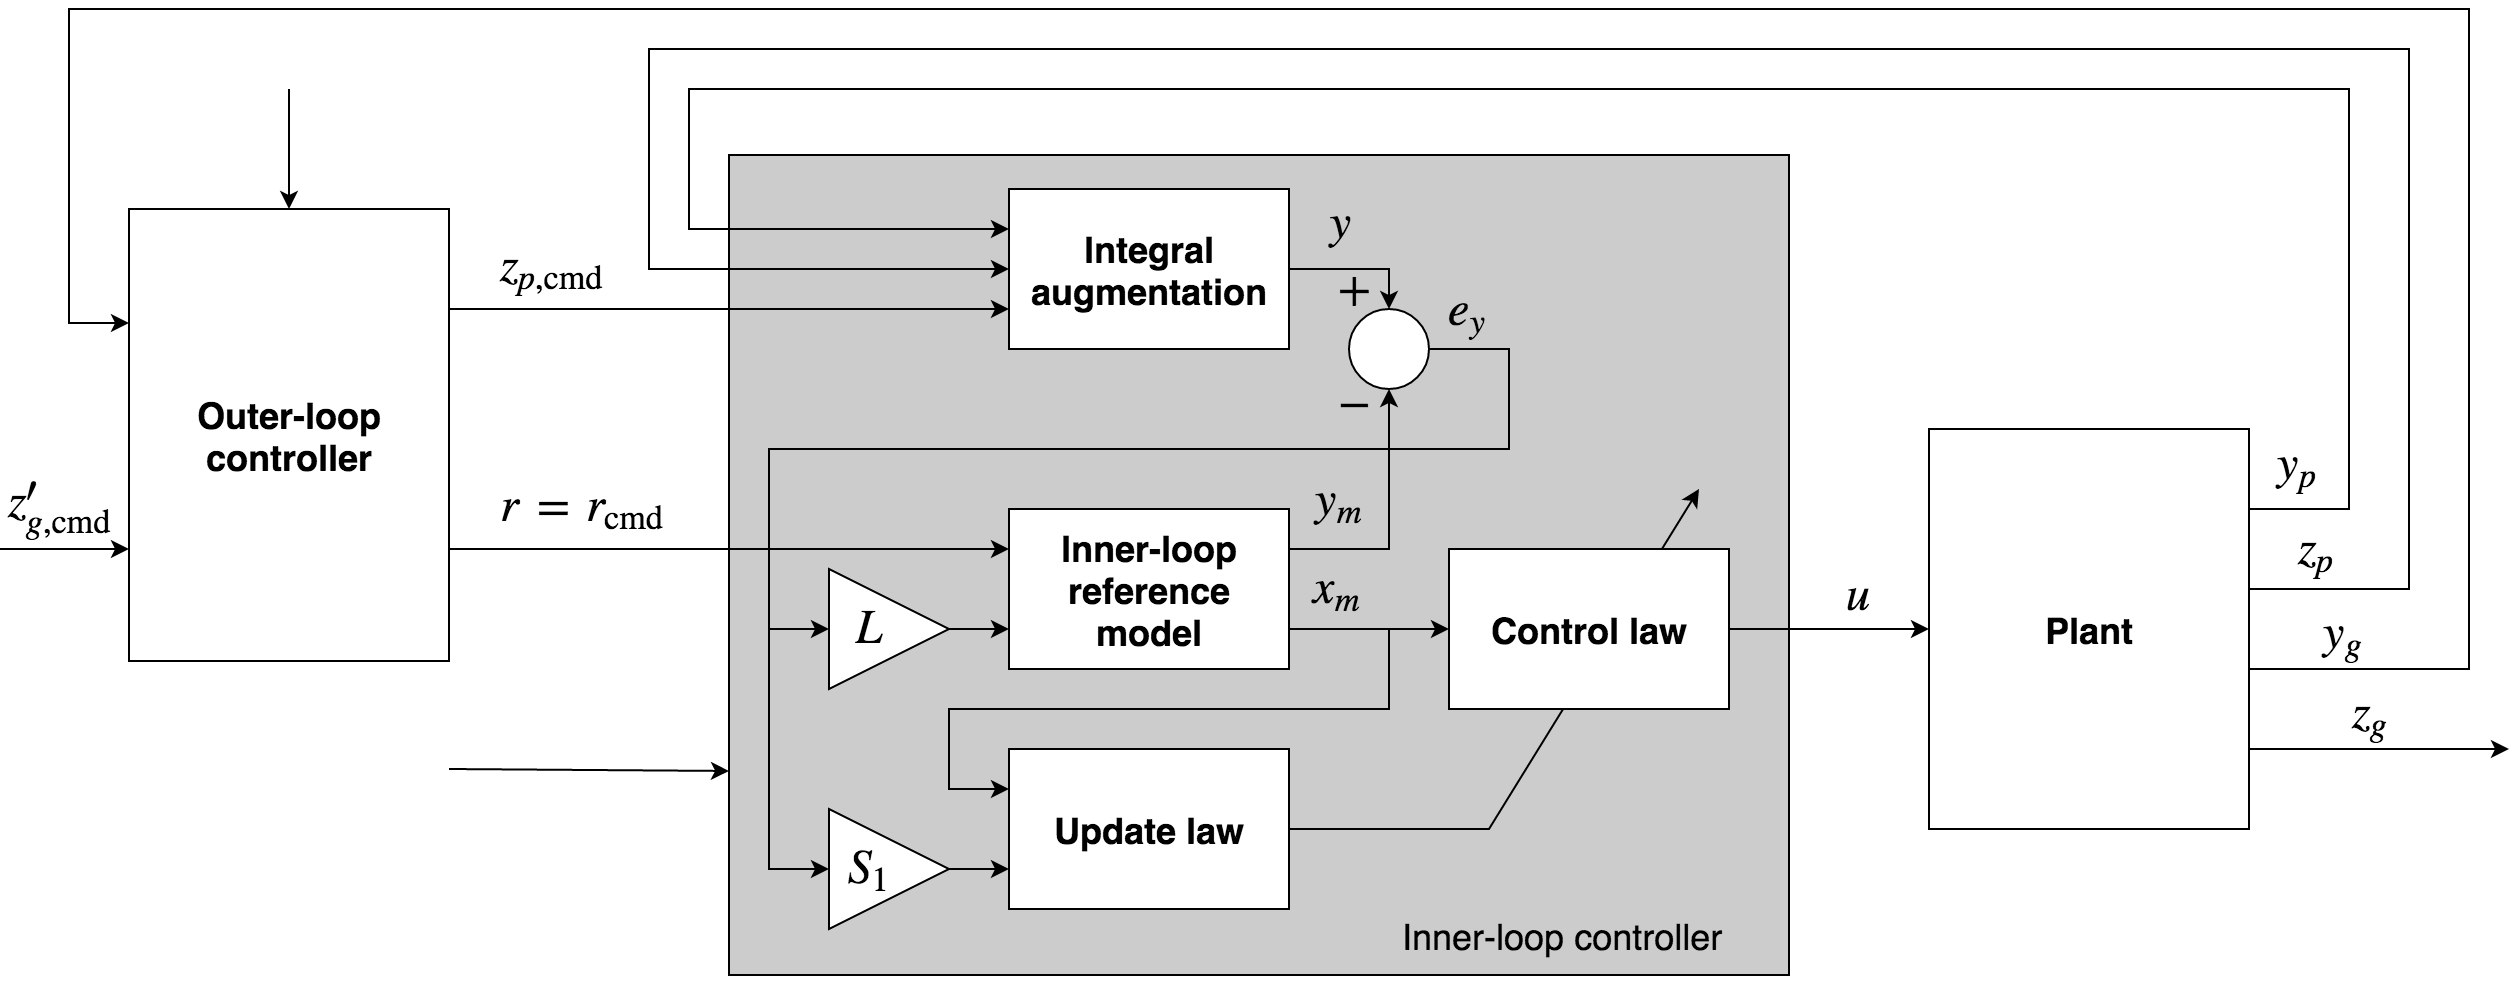
\includegraphics[width=6.5in]{\figurepath/innerLoopWithStartOfOuterLoop.png}
    \vspace{-0.1in}
    \caption{Outer-loop control architecture block diagram.\label{fig.innerLoopWithStartOfOuterLoop}}
  \end{center}
\end{figure}

\section{Outer-Loop Control Architecture}

In this section the outer-loop control architecture is proposed, which consists of two additional reference model components, and some additional outer-loop static feedback gains, two of which are CRM gains.
This architecture is presented, and conditions on the selection of the feedback gains to guarantee global stability of the closed-loop system is given.

In designing the outer-loop controller, the Assumption that $B_{gd}$ in\ \eqref{eqn.innerLoopDynamicsUncertain} is zero is relaxed.
By including the $B_{gd}$ term in\ \eqref{eqn.innerLoopDynamicsUncertain} and using the same integral augmentation, the system in\ \eqref{eqn.uncsystem} becomes
\begin{equation}
  \label{eqn.uncsystemWithBd}
  \begin{split}
    \dot{x}(t) &= Ax(t) + B\bigr(\Lambda u(t)+\Psi^{\top}x(t)\bigr)+B_{\text{cmd}}z_{p,\text{cmd}}(t) + B_{d}x_{g}(t) \\
    y(t) &= Cx(t) \\
  \end{split}
\end{equation}
where $B_{d}\in\mathbb{R}^{n\times n_{g}}$ is given by
\begin{equation*}
  B_{d} =
  \begin{bmatrix}
    B_{gd} \\
    0_{n_{ep}\times n_{g}} \\
  \end{bmatrix}
\end{equation*}
To accommodate the $B_{d}$ term in\ \eqref{eqn.uncsystemWithBd}, the inner-loop reference model in\ \eqref{eqn.refmodel} is modified as
\begin{equation}
  \label{eqn.refmodelWithBd}
  \begin{split}
    \dot{x}_{m}(t) &= A_{m}x_{m}(t) + B_{\text{cmd}}r(t) + L\bigr(y_{m}(t)-y(t)\bigr) + B_{d}x_{gm}(t) \\
    y_{m}(t) &= Cx_{m}(t)
  \end{split}
\end{equation}
This change with the addition of the $B_{d}$ term in the plant in\ \eqref{eqn.uncsystemWithBd} and reference model in\ \eqref{eqn.refmodelWithBd} modifies the inner-loop error dynamics in\ \eqref{eqn.errordynamics1} as follows
\begin{equation}
  \label{eqn.errordynamics4}
  \begin{split}
    \dot{e}_{x}(t) &= (A+LC+B\Psi^{\top})e_{x}(t)+B\Lambda\widetilde{\Theta}^{\top}(t)x_{m}(t) + B_{\text{cmd}}\bigr(z_{p,\text{cmd}}(t) - r(t)\bigr) + B_{d}e_{g}(t) \\
    e_{y}(t) &= Ce_{x}(t) \\
  \end{split}
\end{equation}
The next step is to consider the outer-loop dynamics in\ \eqref{eqn.outerLoopDynamics} and generate the reference signals $r(t)$ and $z_{p,\text{cmd}}(t)$ in\ \eqref{eqn.errordynamics4} so that $z_{g}(t)$ tracks $z_{g,\text{cmd}}(t)$ with bounded errors.
Asymptotic tracking of an arbitrary bounded command $z_{g,\text{cmd}}(t)$ by $z_{g}(t)$ is not possible.
However, in the same way that the inner-loop reference model essentially serves as a command pre-filter for $z_{p,\text{cmd}}(t)$ generating $z_{pm}(t)$ for which asymptotic tracking by $z_{p}(t)$ is possible, a similar filtered version of $z_{g,\text{cmd}}(t)$ for which asymptotic tracking is possible, is created.
For this, some additional outer-loop reference model components are required.

\subsection{Reference Model Design}

\subsubsection{Outer-Loop Reference Model}

An additional outer-loop reference model is introduced in addition to the inner-loop reference model in\ \eqref{eqn.refmodelWithBd} as
\begin{equation}
  \label{eqn.refmodelouter}
  \begin{split}
    \dot{x}_{gm}(t) &= A_{g}x_{gm}(t) + B_{g}x_{m}(t) + L_{y}\bigr(y_{m}(t)-y(t)\bigr) + L_{g}\bigr(y_{gm}(t)-y_{g}(t)\bigr) \\
    y_{gm}(t) &= C_{g}x_{gm}(t) \\
    z_{gm}(t) &= C_{gz}x_{gm}(t) \\
  \end{split}
\end{equation}
where $L_{y}\in\mathbb{R}^{n_{g}\times p}$, and $L_{g}\in\mathbb{R}^{n_{g}\times p_{g}}$.
The outer-loop tracking error is given by
\begin{equation*}
  e_{g}(t) = x_{g}(t) - x_{gm}(t)
\end{equation*}
and the measured outer-loop error by
\begin{equation*}
  e_{gy}(t) = y_{g}(t) - y_{gm}(t)
\end{equation*}
and the goal is to design an outer-loop controller such that $\lim_{t\rightarrow\infty}e_{g}(t)=0$, which will thus enforce the outer-loop tracking as desired.

\begin{rem-dan}\label{rem.ygmandzgm}
  With the structure of the measured and regulated outputs in the outer-loop reference model component\ \eqref{eqn.refmodelouter} where unlike the inner-loop reference model\ \eqref{eqn.refmodel} the regulated output has no direct feedthrough, the measured output matrix is selected so as to contain the regulated output as well.
  That is, the matrix $C_{g}$ in\ \eqref{eqn.refmodelouter} is expressed as
  \begin{equation*}
    C_{g} =
    \begin{bmatrix}
      C_{gy} \\
      C_{gz}
    \end{bmatrix}
  \end{equation*}
\end{rem-dan}

Subtracting the outer-loop dynamics\ \eqref{eqn.outerLoopDynamics} and the outer-loop reference model\ \eqref{eqn.refmodelouter} gives the following outer-loop error dynamics
\begin{equation*}
  \begin{split}
    \dot{e}_{g}(t) &=
    A_{g}x_{g}(t)
    + B_{g}x(t)
    - A_{g}x_{gm}(t)
    - B_{g}x_{m}(t)
    - L_{y}\bigr(y_{m}(t)-y(t)\bigr)
    - L_{g}\bigr(y_{gm}(t)-y_{g}(t)\bigr) \\
    &=
    A_{g}\bigr(x_{g}(t) - x_{gm}(t)\bigr)
    + B_{g}\bigr(x(t) - x_{m}(t)\bigr)
    + L_{y}C\bigr(x(t)-x_{m}(t)\bigr)
    + L_{g}C_{g}\bigr(x_{g}(t)-x_{gm}(t)\bigr) \\
    &=
    A_{g}e_{g}(t)
    + B_{g}e_{x}(t)
    + L_{y}Ce_{x}(t)
    + L_{g}C_{g}e_{g}(t)
  \end{split}
\end{equation*}
giving
\begin{equation}
  \label{eqn.outerlooperrordynamics}
  \begin{split}
    \dot{e}_{g}(t) &= \bigr(A_{g} + L_{g}C_{g}\bigr)e_{g}(t) + \bigr(B_{g} + L_{y}C\bigr)e_{x}(t) \\
    e_{gy}(t) &= C_{g}e_{g}(t) \\
  \end{split}
\end{equation}

\subsubsection{Forward-loop Reference Model}

Combining the inner-loop reference model in\ \eqref{eqn.refmodelWithBd} and the outer-loop reference model in\ \eqref{eqn.refmodelouter}, the combined reference model is obtained as
\begin{equation}
  \label{eqn.refmodelcombined}
  \begin{split}
    \begin{bmatrix}
      \dot{x}_{m}(t) \\
      \dot{x}_{gm}(t) \\
    \end{bmatrix}
    &=
    \begin{bmatrix}
      A_{m} & B_{d} \\
      B_{g} & A_{g} \\
    \end{bmatrix}
    \begin{bmatrix}
      x_{m}(t) \\
      x_{gm}(t) \\
    \end{bmatrix}
    +
    \begin{bmatrix}
      B_{\text{cmd}} \\
      0
    \end{bmatrix} r(t)
    +
    \begin{bmatrix}
      L \\
      L_{y}
    \end{bmatrix}\bigr(y_{m}(t)-y(t)\bigr)
    +
    \begin{bmatrix}
      0 \\
      L_{g}
    \end{bmatrix}\bigr(y_{gm}(t)-y_{g}(t)\bigr) \\
    z_{gm}(t) &=
    \begin{bmatrix}
      0 & C_{gz}
    \end{bmatrix}
    \begin{bmatrix}
      x_{m}(t) \\
      x_{gm}(t) \\
    \end{bmatrix}
  \end{split}
\end{equation}
The forward-loop controller which generates the reference model input command $r(t)$ from the outer-loop command signal $z_{g,\text{cmd}}^{\prime}(t)$ is now designed.
Furthermore, this forward-loop reference model must ensure the complete resulting reference model, given by Eq.\ \eqref{eqn.refmodelcombined} with the forward-loop reference model, is stable.
A control of the follow form is selected
\begin{equation}
  \label{eqn.forwardloopcontroller}
  \begin{split}
    \dot{x}_{fm}(t) &= A_{fm}x_{fm}(t) + B_{f1}z_{g,\text{cmd}}(t) + B_{f2}x_{gm}(t) + B_{f3}x_{m}(t) \\
    r_{\text{cmd}}(t) &= C_{fm}x_{fm}(t) + D_{f1}z_{g,\text{cmd}}(t) + D_{f2}x_{gm}(t) + D_{f3} x_{m}(t) \\
  \end{split}
\end{equation}
where the matrices $A_{fm}\in\mathbb{R}^{n_{f}\times n_{f}}$, $B_{f1}\in\mathbb{R}^{n_{f}\times n_{eg}}$, $B_{f2}\in\mathbb{R}^{n_{f}\times n_{g}}$, $B_{f3}\in\mathbb{R}^{n_{f}\times n}$, $C_{fm}\in\mathbb{R}^{n_{ep}\times n_{f}}$, $D_{f1}\in\mathbb{R}^{n_{ep}\times n_{eg}}$, $D_{f2}\in\mathbb{R}^{n_{ep}\times n_{g}}$, and $D_{f3}\in\mathbb{R}^{n_{ep}\times n}$ are selected so the closed loop system given by combining\ \eqref{eqn.forwardloopcontroller} and\ \eqref{eqn.refmodelcombined} provides steady-state command tracking of $z_{g,\text{cmd}}(t)$ by $z_{gm}(t)$ when the errors $e_{y}(t)$ and $e_{gy}(t)$ are zero.
Furthermore, we set the outer-loop command $z_{g,\text{cmd}}(t)$ in\ \eqref{eqn.forwardloopcontroller} equal to the desired outer-loop command $z_{g,\text{cmd}}^{\prime}(t)$ as
\begin{equation}
  \label{eqn.zgcmdzgcmdprime}
  z_{g,\text{cmd}}(t) = z_{g,\text{cmd}}^{\prime}(t)
\end{equation}
Set $r(t)$ in\ \eqref{eqn.refmodelcombined} using the output from the forward-loop reference model component in\ \eqref{eqn.forwardloopcontroller} as
\begin{equation}
  \label{eqn.rrcmd}
  r(t) = r_{\text{cmd}}(t)
\end{equation}
Substituting the forward-loop controller\ \eqref{eqn.forwardloopcontroller} into\ \eqref{eqn.refmodelcombined} gives the following
\begin{equation}
  \label{eqn.fullOpenLoopReferenceModel}
  \begin{split}
    \begin{bmatrix}
      \dot{x}_{m}(t) \\
      \dot{x}_{gm}(t) \\
      \dot{x}_{fm}(t) \\
    \end{bmatrix}
    &=
    \begin{bmatrix}
      A_{m} & B_{d} & 0 \\
      B_{g} & A_{g} & 0 \\
      B_{f3} & B_{f2} & A_{fm} \\
    \end{bmatrix}
    \begin{bmatrix}
      x_{m}(t) \\
      x_{gm}(t) \\
      x_{fm}(t) \\
    \end{bmatrix}
    +
    \begin{bmatrix}
      B_{\text{cmd}} \\
      0 \\
      0 \\
    \end{bmatrix} r(t)
    +
    \begin{bmatrix}
      L \\
      L_{y} \\
      0 \\
    \end{bmatrix}\bigr(y_{m}(t)-y(t)\bigr) \\
    & \qquad +
    \begin{bmatrix}
      0 \\
      L_{g} \\
      0 \\
    \end{bmatrix}\bigr(y_{gm}(t)-y_{g}(t)\bigr)
    +
    \begin{bmatrix}
      0 \\
      0 \\
      B_{f1} \\
    \end{bmatrix}z_{g,\text{cmd}}(t) \\
    r_{\text{cmd}}(t)
    &=
    \begin{bmatrix}
      D_{f3} & D_{f2} & C_{fm}
    \end{bmatrix}
    \begin{bmatrix}
      x_{m}(t) \\
      x_{gm}(t) \\
      x_{fm}(t) \\
    \end{bmatrix}
    + D_{f1}z_{g,\text{cmd}}(t) \\
  \end{split}
\end{equation}
The entire complete reference model\ \eqref{eqn.fullOpenLoopReferenceModel} can be written more compactly as
\begin{equation}
  \label{eqn.xbareqnopenloop}
  \begin{split}
    \dot{\bar{x}}_{m}(t) &= \bar{A}\bar{x}_{m}(t) + \bar{B}r(t) - \bar{L}_{y}e_{y}(t) - \bar{L}_{g}e_{gy}(t) + \bar{B}_{m}z_{g,\text{cmd}}(t) \\
    r_{\text{cmd}}(t) &= \bar{C}_{m}\bar{x}_{m}(t) + D_{f1}z_{g,\text{cmd}}(t) \\
  \end{split}
\end{equation}
where the entire reference model state $\bar{x}_{m}(t)\in\mathbb{R}^{n+n_{g}+n_{f}}$ is given by
\begin{equation*}
  \bar{x}_{m}(t) =
  \begin{bmatrix}
    x_{m}^{\top}(t) & x_{gm}^{\top}(t) & x_{fm}^{\top}(t)
  \end{bmatrix}^{\top}
\end{equation*}
and where $\bar{A}\in\mathbb{R}^{n+n_{g}+n_{f}\times n+n_{g}+n_{f}}$, $\bar{B}\in\mathbb{R}^{n+n_{g}+n_{f}\times n_{ep}}$, $\bar{L}_{y}\in\mathbb{R}^{n+n_{g}+n_{f}\times p}$, $\bar{L}_{g}\in\mathbb{R}^{n+n_{g}+n_{f}\times p_{g}}$, $\bar{B}_{m}\in\mathbb{R}^{n+n_{g}+n_{f}\times n_{eg}}$, and $\bar{C}_{m}\in\mathbb{R}^{n_{ep} \times n+n_{g}+n_{f}}$ are given by
\begin{equation*}
  \begin{gathered}
    \bar{A} =
    \begin{bmatrix}
      A_{m} & B_{d} & 0 \\
      B_{g} & A_{g} & 0 \\
      B_{f3} & B_{f2} & A_{fm} \\
    \end{bmatrix}
    \quad
    \bar{B} =
    \begin{bmatrix}
      B_{\text{cmd}} \\
      0 \\
      0 \\
    \end{bmatrix}
    \quad
    \bar{L}_{y} =
    \begin{bmatrix}
      L \\
      L_{y} \\
      0 \\
    \end{bmatrix}
    \quad
    \bar{L}_{g} =
    \begin{bmatrix}
      0 \\
      L_{g} \\
      0 \\
    \end{bmatrix}
    \quad
    \bar{B}_{m} =
    \begin{bmatrix}
      0 \\
      0 \\
      B_{f1} \\
    \end{bmatrix} \\
    \bar{C}_{m} =
    \begin{bmatrix}
      D_{f3} & D_{f2} & C_{fm}
    \end{bmatrix}
  \end{gathered}
\end{equation*}
Setting the inner-loop reference model command $r(t)$ as in\ \eqref{eqn.rrcmd} and simplifying\ \eqref{eqn.fullOpenLoopReferenceModel} gives
\begin{equation}
  \label{eqn.refmodelcombinedwithforwardloop}
  \begin{split}
    \begin{bmatrix}
      \dot{x}_{m}(t) \\
      \dot{x}_{gm}(t) \\
      \dot{x}_{fm}(t) \\
    \end{bmatrix}
    &=
    \begin{bmatrix}
      A_{m}+B_{\text{cmd}}D_{f3} & B_{d} + B_{\text{cmd}}D_{f2} & B_{\text{cmd}}C_{fm} \\
      B_{g} & A_{g} & 0 \\
      B_{f3} & B_{f2} & A_{fm} \\
    \end{bmatrix}
    \begin{bmatrix}
      x_{m}(t) \\
      x_{gm}(t) \\
      x_{fm}(t)
    \end{bmatrix}
    +
    \begin{bmatrix}
      B_{\text{cmd}}D_{f1} \\
      0 \\
      B_{f1} \\
    \end{bmatrix} z_{g,\text{cmd}}(t) \\
    &\quad+
    \begin{bmatrix}
      L \\
      L_{y} \\
      0 \\
    \end{bmatrix}\bigr(y_{m}(t)-y(t)\bigr)
    +
    \begin{bmatrix}
      0 \\
      L_{g} \\
      0 \\
    \end{bmatrix}\bigr(y_{gm}(t)-y_{g}(t)\bigr) \\
    r(t)
    &=
    \begin{bmatrix}
      D_{f3} & D_{f2} & C_{fm}
    \end{bmatrix}
    \begin{bmatrix}
      x_{m}(t) \\
      x_{gm}(t) \\
      x_{fm}(t) \\
    \end{bmatrix}
    + D_{f1}z_{g,\text{cmd}}(t) \\
  \end{split}
\end{equation}
which can be represented more compactly as
\begin{equation}
  \label{eqn.compactreferencemodel}
  \begin{split}
    \dot{\bar{x}}_{m}(t) &= \bar{A}_{m}\bar{x}_{m}(t) + \bar{B}_{\text{cmd}}z_{g,\text{cmd}}(t) - \bar{L}_{y}e_{y}(t) - \bar{L}_{g}e_{gy}(t) \\
    r_{\text{cmd}}(t) &= \bar{C}_{m}\bar{x}_{m}(t) + D_{f1}z_{g,\text{cmd}}(t) \\
  \end{split}
\end{equation}
where $\bar{A}_{m}\in\mathbb{R}^{n+n_{g}+n_{f}\times n+n_{g}+n_{f}}$ and $\bar{B}_{\text{cmd}}\in\mathbb{R}^{n+n_{g}+n_{f}\times n_{eg}}$ are given by
\begin{equation}
  \bar{A}_{m} =
  \begin{bmatrix}
    A_{m}+B_{\text{cmd}}D_{f3} & B_{d} + B_{\text{cmd}}D_{f2} & B_{\text{cmd}}C_{fm} \\
    B_{g} & A_{g} & 0 \\
    B_{f3} & B_{f2} & A_{fm} \\
  \end{bmatrix}
  \qquad
  \bar{B}_{\text{cmd}} =
  \begin{bmatrix}
    B_{\text{cmd}}D_{f1} \\
    0 \\
    B_{f1} \\
  \end{bmatrix}
\end{equation}
where $\bar{A}_{m} = \bar{A}+\bar{B}\bar{C}_{m}$.
Appropriate selection of the controller in\ \eqref{eqn.forwardloopcontroller} ensures that $\bar{A}_{m}$ in\ \eqref{eqn.compactreferencemodel} is Hurwitz.
Combining the integral augmented, uncertain inner-loop dynamics in\ \eqref{eqn.uncsystemWithBd} with the outer-loop guidance dynamics\ \eqref{eqn.outerLoopDynamics} and reference model\ \eqref{eqn.compactreferencemodel} the following system is obtained
\begin{equation}
  \label{eqn.plantAndCompactReferenceModel}
  \begin{aligned}
    \dot{x}(t)
    &=
    Ax(t) + B\bigr(\Lambda u(t)+\Psi^{\top}x(t)\bigr) + B_{\text{cmd}}z_{p,\text{cmd}}(t) + B_{d}x_{g}(t) \\
    y(t)
    &=
    Cx(t) \\
    \dot{x}_{g}(t)
    &=
    A_{g}x_{g}(t) + B_{g}x(t) \\
    y_{g}(t)
    &=
    C_{g}x_{g}(t) \\
    \dot{\bar{x}}_{m}
    &=
    \bar{A}_{m}\bar{x}_{m}(t) + \bar{B}_{\text{cmd}}z_{g,\text{cmd}}(t) - \bar{L}_{y}e_{y}(t) - \bar{L}_{g}e_{gy}(t) \\
    r_{\text{cmd}}
    &=
    \bar{C}_{m}\bar{x}_{m}(t) + D_{f1}z_{g,\text{cmd}}(t)
  \end{aligned}
\end{equation}
where only the specification of $z_{p,\text{cmd}}(t)$ remains to completely specify the control architecture.

\begin{rem-dan}
  One possible selection for the forward-loop reference model in\ \eqref{eqn.forwardloopcontroller} is that of an LQR-PI controller as used in the inner-loop design.
  When using such a controller,\ \eqref{eqn.forwardloopcontroller} becomes
  \begin{equation}
    \label{eqn.rKbar}
    \begin{split}
      \dot{x}_{fm}(t) &= z_{g,\text{cmd}}(t) - z_{gm}(t) \\
      r_{\text{cmd}}(t) &= \bar{K}^{\top}\bar{x}_{m}(t) \\
    \end{split}
  \end{equation}
  where $\bar{K}\in\mathbb{R}^{n+n_{g}+n_{f} \times n_{ep}}$ is given by
  \begin{equation}
    \label{eqn.Kbar}
    \bar{K} =
    \begin{bmatrix}
      D_{f3} & D_{f2} & C_{fm}
    \end{bmatrix}^{\top}
  \end{equation}
  with $n_{f} = n_{eg}$ and where the remaining matrices which define the forward-loop reference model in\ \eqref{eqn.forwardloopcontroller} are selected as follows
  \begin{equation}
    A_{fm} = 0
    \qquad
    B_{f1} = I
    \qquad
    B_{f2} = C_{gz}
    \qquad
    B_{f3} = 0
    \qquad
    D_{f1} = 0
  \end{equation}
  and $C_{fm}$, $D_{f2}$, and $D_{f3}$ in\ \eqref{eqn.Kbar} are selected using LQR.\@
\end{rem-dan}

\subsection{Generating the Inner-Loop Command}

The command input to the plant $z_{p,\text{cmd}}(t)$ in\ \eqref{eqn.zcmd1}, with the inner-loop reference model input given by $r(t)=r_{\text{cmd}}(t)$ as in\ \eqref{eqn.rrcmd}, is modified with an outer-loop error feedback term as follows
\begin{equation}
  \label{eqn.zpcmd}
  z_{p,\text{cmd}}(t) = r (t)+ e_{gs}(t)
\end{equation}
where
\begin{equation}
  \label{eqn.egs}
  e_{gs}(t) = S_{g}e_{gy}(t)
\end{equation}
and $S_{g}\in\mathbb{R}^{n_{ep}\times p_{g}}$.
This choice of $z_{p,\text{cmd}}(t)$ modifies the inner-loop error dynamics in\ \eqref{eqn.errordynamics4} as
\begin{equation}
  \label{eqn.errordynamics5}
  \begin{split}
    \dot{e}_{x}(t)
    &=
    \bigr(A+LC+B\Psi^{\top}\bigr)e_{x}(t) + B\Lambda\widetilde{\Theta}^{\top}(t)x_{m}(t) + \bigr(B_{\text{cmd}}S_{g}C_{g} + B_{d}\bigr)e_{g}(t) \\
    e_{y}(t)
    &=
    Ce_{x}(t) \\
  \end{split}
\end{equation}
The proposed control architecture can be represented by the block diagram in Figure~\ref{fig.innerAndOuterLoopDansOutputFeedback}, which groups the components as in\ \eqref{eqn.plantAndCompactReferenceModel} with the reference model separate from the plant, and shows the two additional CRM feedback gains $L_{g}$ and $L_{y}$ in addition to the inner-loop CRM gain $L$.
Alternatively, the architecture can be represented as in Figure~\ref{fig.innerAndOuterLoopExplicit} which better shows the grouping of both reference model and control into their inner and outer-loop components.

\begin{figure}[H]
  \begin{center}
    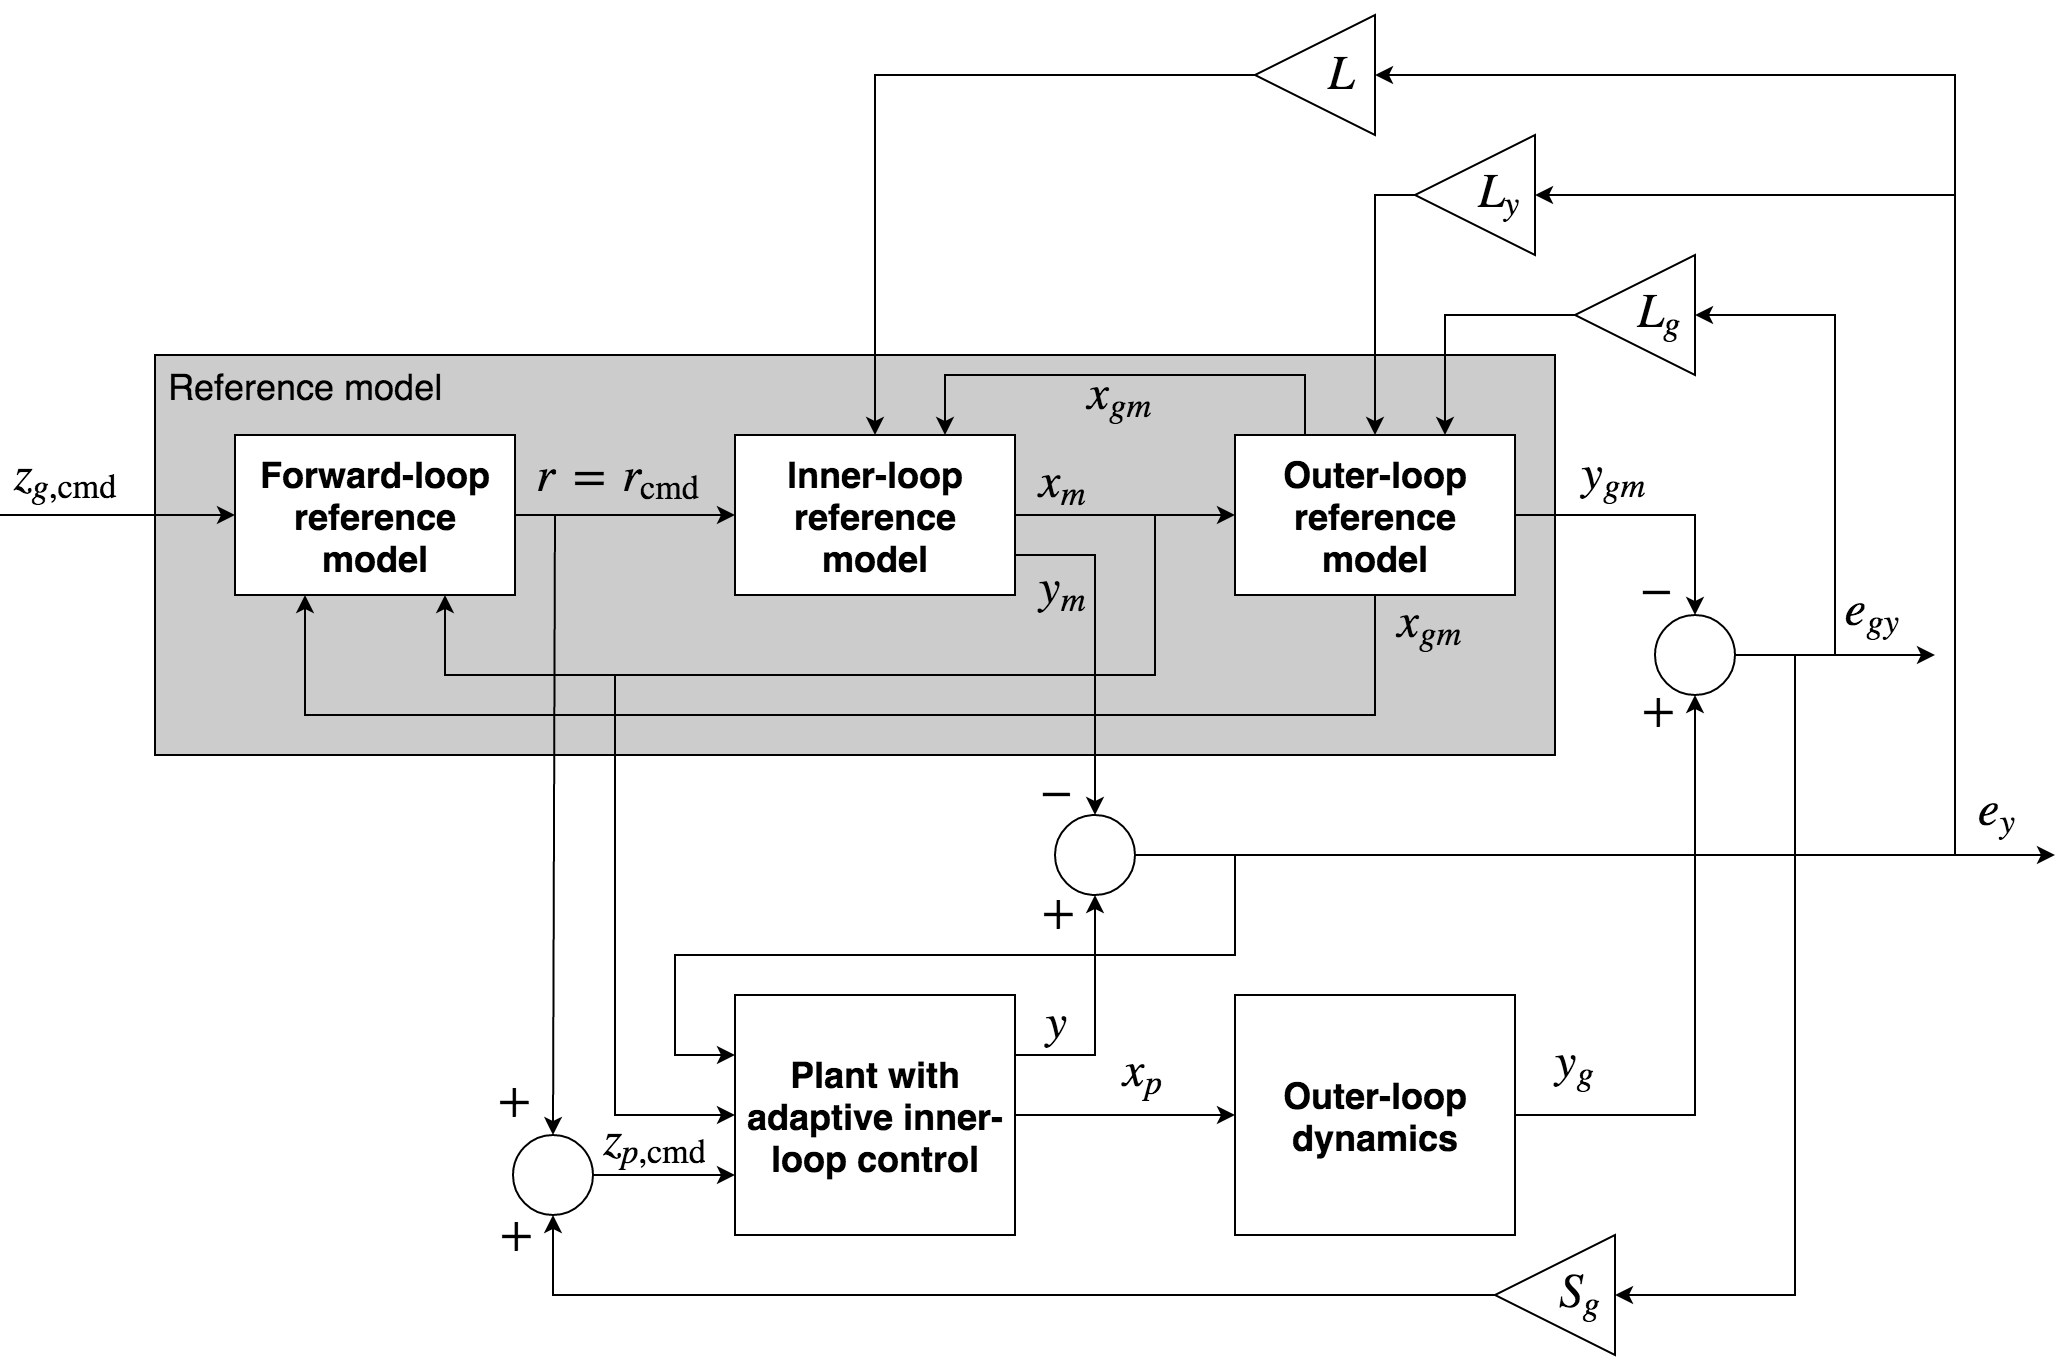
\includegraphics[width=6.5in]{\figurepath/innerAndOuterLoopDansOutputFeedback2.png}
    \vspace{-0.1in}
    \caption{Complete integrated inner and outer-loop design block diagram.\label{fig.innerAndOuterLoopDansOutputFeedback}}
  \end{center}
\end{figure}

\begin{figure}[H]
  \begin{center}
    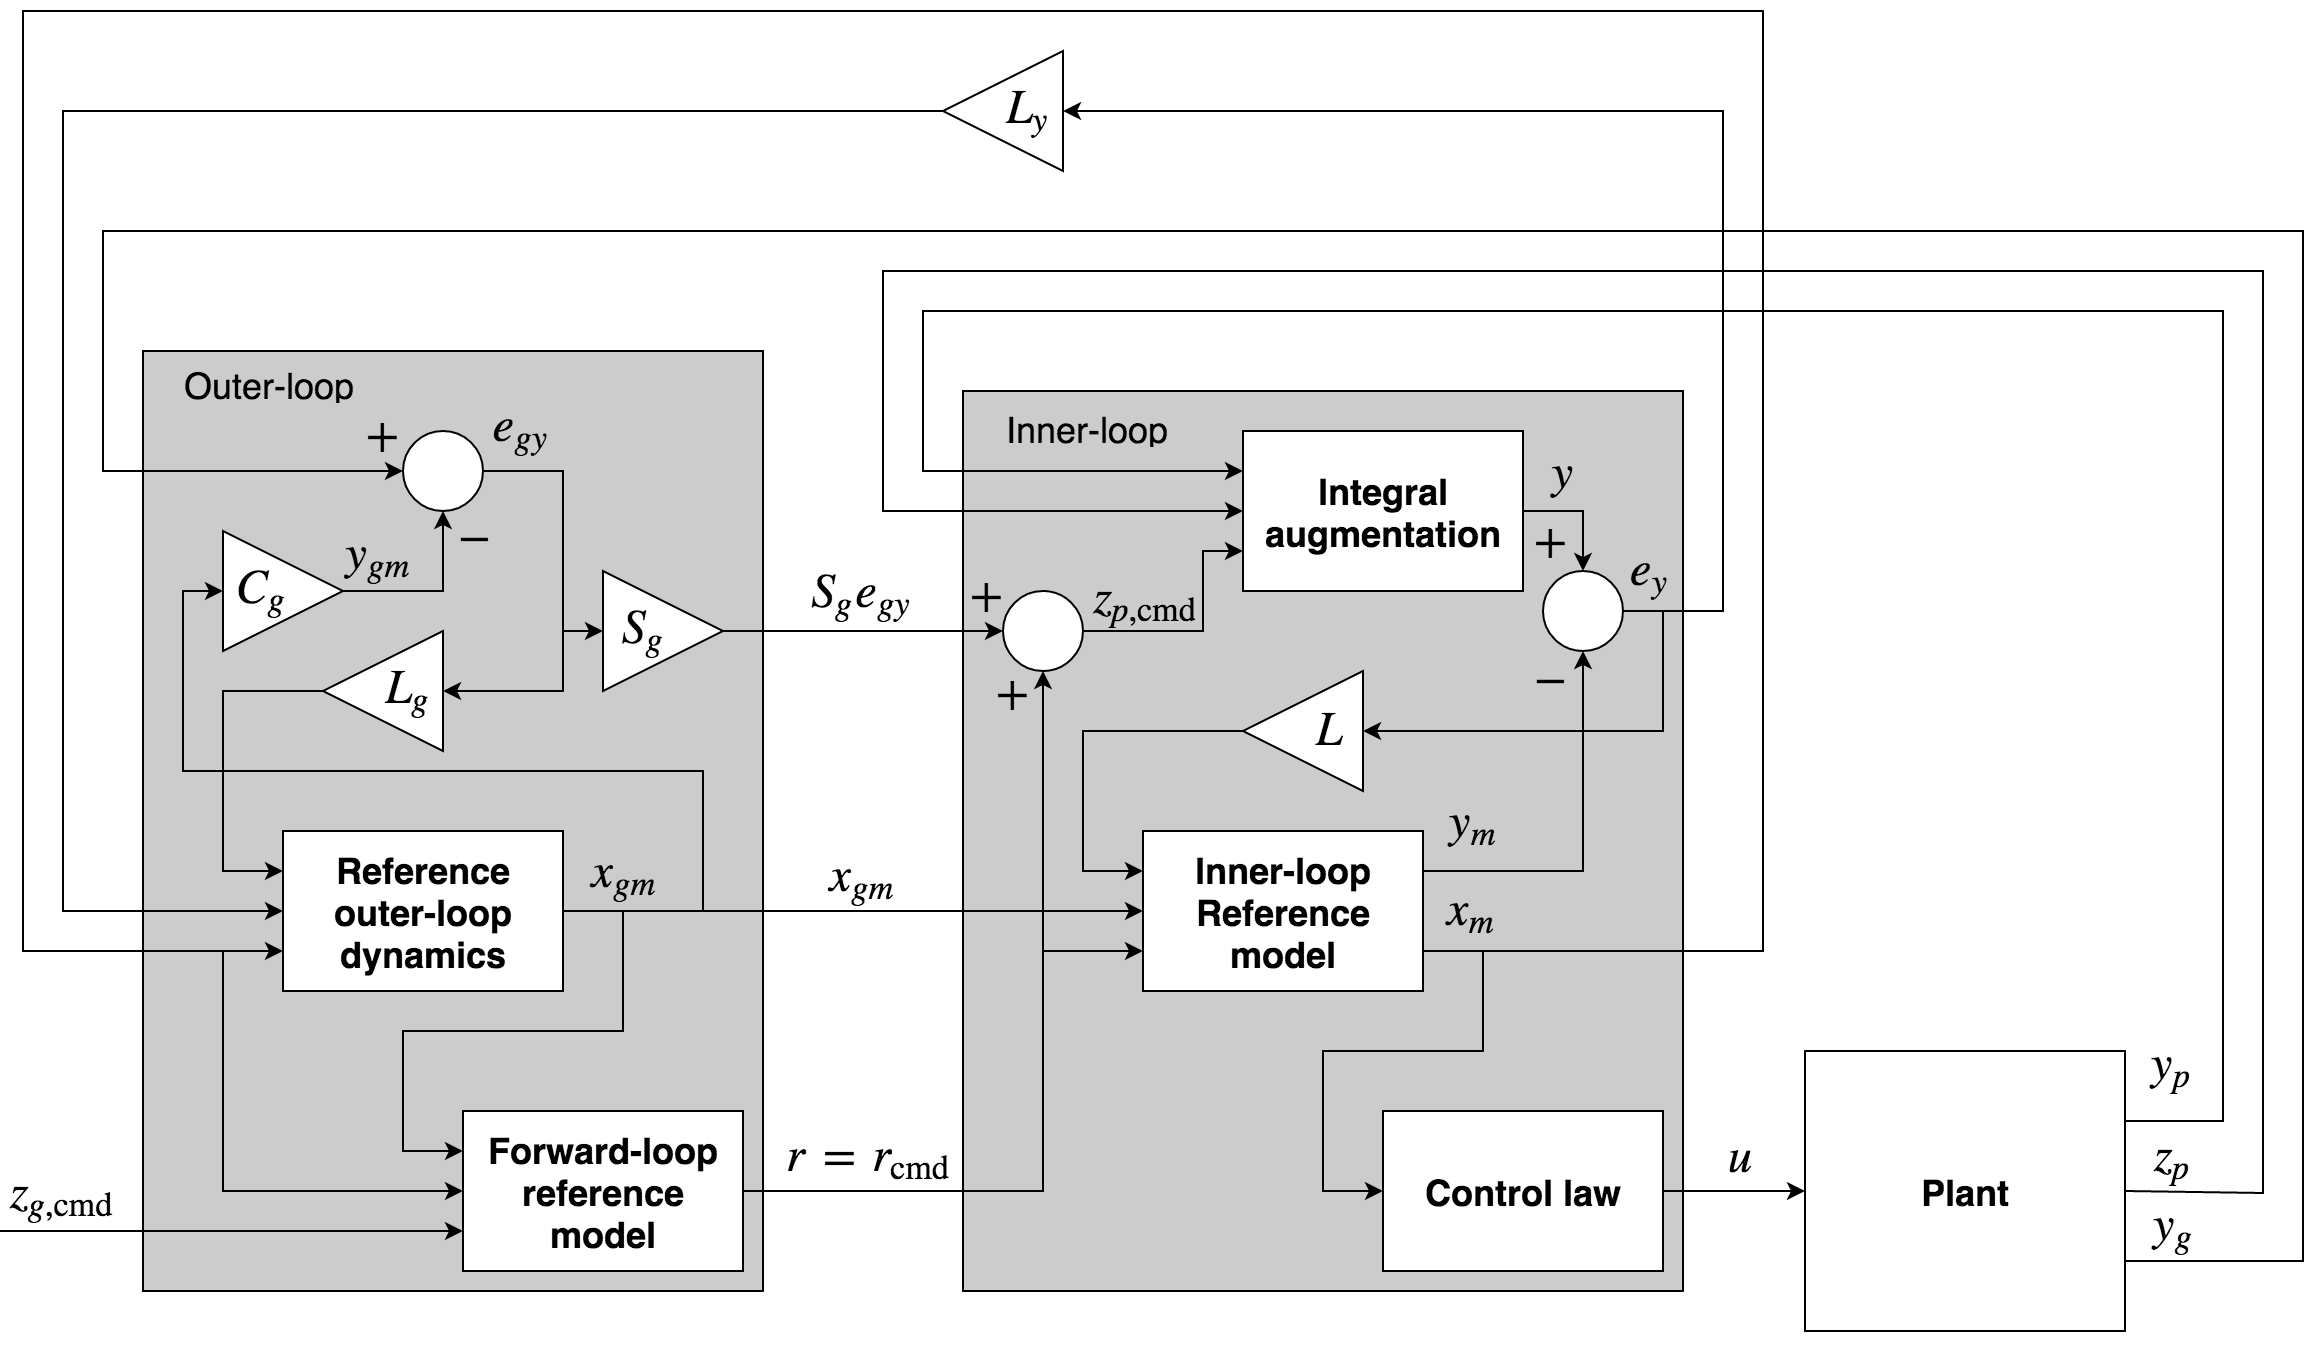
\includegraphics[width=6.5in]{\figurepath/innerAndOuterLoopExplicit.png}
    \vspace{-0.1in}
    \caption{Complete integrated inner and outer-loop design block diagram.\label{fig.innerAndOuterLoopExplicit}}
  \end{center}
\end{figure}

In the most simple form, the block diagram in Figure~\ref{fig.innerAndOuterLoopExplicit} can be represented using the block diagram in Figure~\ref{fig.simpleBlockWithoutLimiter} where $x(t)$ represents the feedback of the plant and inner-loop reference model outputs and contains $y_{g}(t)$, $e_{y}(t)$, and $x_{m}(t)$.
The signal $e(t)$ contains the outer-loop error $e_{gs}(t)$ and the outer-loop reference model state $x_{gm}(t)$.

\begin{figure}[H]
  \begin{center}
    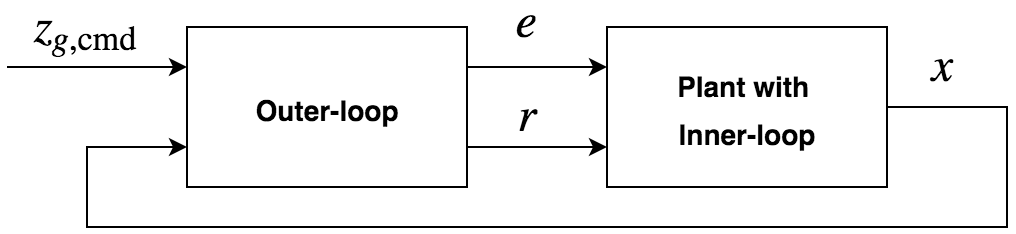
\includegraphics[width=4.5in]{\figurepath/simpleBlockWithoutLimiter.png}
    \vspace{-0.1in}
    \caption{Simplified inner and outer-loop block diagram.\label{fig.simpleBlockWithoutLimiter}}
  \end{center}
\end{figure}

The above sections have presented the inner-loop control design and the outer-loop architecture including the forward-loop reference model.
Combining the inner-loop error dynamics in\ \eqref{eqn.errordynamics4} with the outer-loop error dynamics in\ \eqref{eqn.outerlooperrordynamics} with $z_{p,\text{cmd}}(t)$ given by\ \eqref{eqn.zpcmd} and\ \eqref{eqn.egs} the following inner and outer-loop error dynamics are obtained
\begin{equation}
  \label{eqn.innerAndOuterLoopErrorDynamics1}
  \begin{split}
    \dot{e}_{x}(t)
    &=
    \bigr(A+LC+B\Psi^{\top}\bigr)e_{x}(t) + B\Lambda\widetilde{\Theta}^{\top}(t)x_{m}(t) + \bigr(B_{\text{cmd}}S_{g}C_{g} + B_{d}\bigr)e_{g}(t) \\
    \dot{e}_{g}(t)
    &=
    \bigr(A_{g} + L_{g}C_{g}\bigr)e_{g}(t) + \bigr(B_{g} + L_{y}C\bigr)e_{x}(t) \\
  \end{split}
\end{equation}
The CRM feedback gains $L_{y}$, $L_{g}$, and $S_{g}$ in\ \eqref{eqn.innerAndOuterLoopErrorDynamics1} need to be selected to guarantee global stability of the closed-loop system.
Looking at these error dynamics provied a cue as to how stability may be achieved, with $L_{g}$ being used to stabilize the outer-loop error dynamics, and $S_{g}$ and $L_{y}$ used to cancel the error cross-coupling terms.
By selecting these outer-loop reference model gains in this way, the error dynamics are essentially reduced to standard adaptive error dynamics on the inner-loop, and stable outer-loop error dynamics.
The specific requirements for stability of the error dynamics in\ \eqref{eqn.innerAndOuterLoopErrorDynamics1} and the resulting conditions leading to the solutions for $S_{g}$, $L_{g}$ and $L_{y}$ are provided in the following subsection.

\subsection{Conditions for Stability}

The complete control architecture is specified by the plant and reference model\ \eqref{eqn.plantAndCompactReferenceModel}, inner-loop command specified by\ \eqref{eqn.zpcmd} and\ \eqref{eqn.egs}, control input\ \eqref{eqn.u}, and update law in\ \eqref{eqn.updatelaw}.
All that remains to complete the control design is to specify solutions to $L_{y}$, $L_{g}$, and $S_{g}$ such that the closed-loop system is stable and the control goal of command tracking is satisfied.
In order to prove stability of the closed-loop system, the matrices $L_{y}$, $S_{g}$, and $P_{g}=P_{g}^{\top}>0$ need to be found satisfying the following condition
\begin{equation}
  \label{eqn.condition1}
  (B_{g}+L_{y}C)^{\top}P_{g} + P_{x}B_{\text{cmd}}S_{g}C_{g} + B_{d} = 0
\end{equation}
where $L_{g}$ must be picked together with $P_{g}$ so that, in addition, the following Lyapunov inequality is satisfied
  \begin{equation}
  \label{eqn.condition2}
  (A_{g}+L_{g}C_{g})^{\top}P_{g}+P_{g}(A_{g}+L_{g}C_{g}) < -Q_{g}
\end{equation}
where $Q_{g}=Q_{g}^{\top}>0$.
Together, the conditions in\ \eqref{eqn.condition1} and\ \eqref{eqn.condition2} can be combined, and the problem restated as: Find the matrices $L_{y}$, $S_{g}$, $L_{g}$ and $P_{g}$ that together satisfy the following conditions
\begin{align}
  \label{eqn.condition3a}
  (B_{g}+L_{y}C)^{\top}P_{g} + P_{x}B_{\text{cmd}}S_{g}C_{g} + B_{d} &= 0 \\
  \label{eqn.condition3b}
  (A_{g}+L_{g}C_{g})^{\top}P_{g}+P_{g}(A_{g}+L_{g}C_{g}) &< -Q_{g}
\end{align}
The condition in Eq.\ \eqref{eqn.condition3a} can be rearranged as
\begin{equation}
  \label{eqn.theEquation}
  C^{\top}L_{y}^{\top} = - P_{x}B_{\text{cmd}}S_{g}C_{g}P_{g}^{-1} - B_{g}^{\top} - B_{d}P_{g}^{-1}
\end{equation}
Examining the condition in\ \eqref{eqn.theEquation} it can be seen that the CRM gain $L_{y}^{\top}$ on the left hand side rotates and scale the columns of $C^{\top}$, but cannot do anything such that the columns of the matrix $C^{\top}L_{y}^{\top}$ are orthogonal to columns of $C^{\top}$.
This means that, in general, $L_{y}$ would not be enough to direct the columns of $C^{\top}$ so as to match the right hand side of\ \eqref{eqn.theEquation}.
Thus $S_{g}$ together with $P_{g}$ must be used to ensure the columns of the right hand side in are in the space spanned by the columns of $C^{\top}$.
That is, $S_{g}$ and $P_{g}$ must be selected such that when\ \eqref{eqn.theEquation} is left-multiplied by $M^{\top}$, that the quantity on the right hand side vanishes, where $M$ is the inner-loop measured output annihilator matrix from\ \eqref{eqn.NB0CM0} that satisfies $CM=0$.
Left multiplying\ \eqref{eqn.theEquation} by $M^{\top}$ and substituting in the expression for $P_{x}$ from\ \eqref{eqn.Px} the following is obtained
\begin{equation}
  \label{eqn.makeMeZero}
  -M^{\top}N^{\top}XNB_{\text{cmd}}S_{g}C_{g}P_{g}^{-1} = M^{\top}(B_{g}^{\top} + B_{d}P_{g}^{-1})
\end{equation}
Furthermore, recall from Lemma~\ref{lem.elimination}, the Matrix Elimination Lemma, for an $L_{g}$ to exist satisfying\ \eqref{eqn.condition3b}, a $P_{g}$ must exist satisfying
\begin{equation}
  \label{eqn.reducedPgInequality}
  C_{g}^{\top\perp\top} (A_{g}^{\top}P_{g} + P_{g}A_{g}) C_{g}^{\top\perp} < 0
\end{equation}
Thus in order to find $L_{y}$, $S_{g}$, and $P_{g}$ satisfying\ \eqref{eqn.theEquation}, and thus\ \eqref{eqn.condition3a}, with the additional constraint that $P_{g}$ solves\ \eqref{eqn.reducedPgInequality}, thus guaranteeing an $L_{g}$ exists that solves\ \eqref{eqn.condition3b}, the matrices $P_{g}$ and $S_{g}$ must be found satisfying
\begin{align}
  \label{eqn.condition4a}
  -M^{\top}N^{\top}XNB_{\text{cmd}}S_{g}C_{g}P_{g}^{-1} &= M^{\top}(B_{g}^{\top} + B_{d}P_{g}^{-1}) \\
  \label{eqn.condition4b}
  C_{g}^{\top\perp\top} (A_{g}^{\top}P_{g} + P_{g}A_{g}) C_{g}^{\top\perp} &< 0
\end{align}
If $S_{g}$ and $P_{g}$ exist satisfying\ \eqref{eqn.condition4a} and\ \eqref{eqn.condition4b}, then the solution to the outer-loop control problem exists.
Once solutions $S_{g}$ and $P_{g}$ are found analytically, an $L_{g}$ satisfying\ \eqref{eqn.condition3b} is guaranteed to exist, which can be simply found it by solving\ \eqref{eqn.condition3b} numerically, as was done to obtain $L$ in the inner-loop design in Chapter~\ref{ch.innerLoop}.
With the solutions $S_{g}$ and $P_{g}$, the solution $L_{y}$ from\ \eqref{eqn.theEquation} is calculated.
So the problem that remains is to find $S_{g}$ and $P_{g}$ satisfying\ \eqref{eqn.condition4a} and\ \eqref{eqn.condition4b}.

\begin{rem-dan}
  If the requirement that the inequality in\ \eqref{eqn.condition3b} be strict is relaxed, then the condition given by\ \eqref{eqn.condition4b} is changed so as not to be a strict inequality either.
\end{rem-dan}

The existence of solutions to\ \eqref{eqn.condition4a} is dependent on the sizes of the matrices.
Based on these different sizes will affect how\ \eqref{eqn.condition4a} is manipulated to get it in a form which can be solved.

\subsubsection{Case I:~$n-p=n_{ep}$}

This case corresponds to the number of inner-loop regulated outputs $n_{ep}$, being equal to the number of unmeasured inner-loop states, given by $n-p$.
In this case, $M^{\top}N^{\top}XNB_{\text{cmd}}$ in\ \eqref{eqn.condition4a} is square, and full rank as specified in Remark~\ref{rem.X12FullRank}, so left-multiply\ \eqref{eqn.condition4a} by $(M^{\top}N^{\top}XNB_{\text{cmd}})^{-1}$ and right-multiply by $P_{g}$ to obtain
\begin{equation}
  \label{eqn.SgCg}
  S_{g}C_{g} = - (M^{\top}N^{\top}XNB_{\text{cmd}})^{-1}M^{\top}(B_{g}^{\top}+B_{d}P_{g}^{-1})P_{g}
\end{equation}
It can be seen from\ \eqref{eqn.SgCg} that $S_{g}$ can only rotate the vectors that make up the rows of $C_{g}$ to other directions within their span.
Thus, it is necessary to make sure that the right hand side of\ \eqref{eqn.SgCg} lies in the same span as the rows of $C_{g}$, then $S_{g}$ can be used to rotate them as required.
For the right hand side to be in the same span as the rows of $C_{g}$, it has to have the same nullspace.
That is, if\ \eqref{eqn.SgCg} is multiplied on the right hand side by $C_{g}^{\top\perp}$ the resulting quantity must be zero.
Thus the goal is to find $P_{g}$ satisfying the following
\begin{equation}
  \label{eqn.PgMustSatisfyCaseI}
  (M^{\top}N^{\top}XNB_{\text{cmd}})^{-1}M^{\top}(B_{g}^{\top}+B_{d}P_{g}^{-1})P_{g}C_{g}^{\top\perp} = 0
\end{equation}
But since $M^{\top}N^{\top}XNB_{\text{cmd}}$ is square and full rank, finding $P_{g}$ satisfying\ \eqref{eqn.PgMustSatisfyCaseI} is equivalent to finding $P_{g}$ satisfying the following equation
\begin{equation}
  \label{eqn.AXBCcase1}
  M^{\top}B_{g}^{\top}P_{g}C_{g}^{\top\perp} = -M^{\top}B_{d}C_{g}^{\top\perp}
\end{equation}
with $M^{\top}B_{g}^{\top}\in\mathbb{R}^{n-p\times n_{g}}$ and $C_{g}^{\top\perp}\in\mathbb{R}^{n_{g}\times n_{g}-p_{g}}$.
Since $C_{g}$ is always wide, $S_{g}$ from\ \eqref{eqn.SgCg} can be solved for using a right inverse of $C_{g}$ to get
\begin{equation}
  \label{eqn.SgCaseI}
  S_{g} = - (M^{\top}N^{\top}XNB_{\text{cmd}})^{-1}M^{\top}(B_{g}^{\top}+B_{d}P_{g}^{-1})P_{g}C_{g}^{-1_{\text{right}}}
\end{equation}

\subsubsection{Case II:~$n-p<n_{ep}$}

This case corresponds to the number of inner-loop regulated outputs $n_{ep}$, being greater than the number of unmeasured inner-loop states, given by $n-p$.
In this case $M^{\top}N^{\top}XNB_{\text{cmd}}$ in\ \eqref{eqn.condition4a} is wide.
A right inverse is used to simplify\ \eqref{eqn.condition4a} as
\begin{equation*}
  S_{g}C_{g}
  =
  -(M^{\top}N^{\top}XNB_{\text{cmd}})^{-1_{\text{right}}}M^{\top}(B_{g}^{\top}+B_{d}P_{g}^{-1})P_{g}
\end{equation*}
As in Case I, $S_{g}$ can only match the right hand side in the span of $C_{g}$, so need to make sure that the right hand side is within the span of $C_{g}$.
So $P_{g}$ must satisfy
\begin{equation}
  \label{eqn.PgMustSatisfyCaseII}
  (M^{\top}N^{\top}XNB_{\text{cmd}})^{-1_{\text{right}}}M^{\top}(B_{g}^{\top}+B_{d}P_{g}^{-1})P_{g}C_{g}^{\top\perp} = 0
\end{equation}
But because $(M^{\top}N^{\top}XNB_{\text{cmd}})^{-1_{\text{right}}}$ is tall and full rank, finding $P_{g}$ satisfying\ \eqref{eqn.PgMustSatisfyCaseII} is equivalent to finding $P_{g}$ satisfying the following equation
\begin{equation}
  \label{eqn.AXBCcase2}
  M^{\top}B_{g}^{\top}P_{g}C_{g}^{\top\perp} = - M^{\top}B_{d}C_{g}^{\top\perp}
\end{equation}
Once $P_{g}$ satisfying\ \eqref{eqn.AXBCcase2} is found, $S_{g}$ is determined by
\begin{equation}
  \label{eqn.SgCaseII}
  S_{g} = - (M^{\top}N^{\top}XNB_{\text{cmd}})^{-1_{\text{right}}}M^{\top}(B_{g}^{\top}+B_{d}P_{g}^{-1})P_{g}C_{g}^{-1_{\text{right}}}
\end{equation}

\subsubsection{Case III:~$n-p>n_{ep}$}

This case corresponds to the number of inner-loop regulated outputs $n_{ep}$, being less than the number of unmeasured inner-loop states, given by $n-p$.
In this case $M^{\top}N^{\top}XNB_{\text{cmd}}$ in\ \eqref{eqn.condition4a} is tall, so $S_{g}$ doesn't have the degrees of freedom to satisfy\ \eqref{eqn.condition4a}.

The conditions for the existence of $S_{g}$ and $P_{g}$ exist satisfying\ \eqref{eqn.condition4a} and\ \eqref{eqn.condition4b} is stated in the following theorem.

\begin{thm-dan}\label{thm.existenceOuterLoop}
  For the existence of $S_{g}$ and $P_{g}$ satisfying\ \eqref{eqn.condition4a} and\ \eqref{eqn.condition4b} for a stable outer-loop controller, the plant must satisfy $n-p\leq n_{ep}$, $n-p<n_{g}$, as well as the following inequality
  \begin{equation}
    \label{eqn.outerLoopTheoremInequality}
    C_{g}^{\top\perp\top}A_{g}^{\top}(B_{g}M)^{\perp}\bigr(C_{g}^{\top\perp\top}(B_{g}M)^{\perp}\bigr)^{-1_{\textnormal{right}}}
    <0
  \end{equation}
\end{thm-dan}

\begin{proof-dan}
  Finding $S_{g}$ and $P_{g}$ satisfying\ \eqref{eqn.condition4a} involves first manipulating\ \eqref{eqn.condition4a} by selecting $P_{g}$ to ensure that $S_{g}$, which acts through the rows of $C_{g}$, will be sufficient to satisfy\ \eqref{eqn.condition4a}.
  This results in a finding the set of all $P_{g}=P_{g}^{\top}>0$ which satisfy $\Pi_{A}P_{g}\Pi_{B}=\Pi_{C}$, where $\Pi_{A}$, $\Pi_{B}$, and $\Pi_{C}$ are matrices which depend on the state-space plant matrices.
  Finding $P_{g}$ involves using a generalized singular value decomposition, and fixes certain elements of $P_{g}$ based on $\Pi_{A}$, $\Pi_{B}$, and $\Pi_{C}$.
  Then, from this set of $P_{g}$, those which also satisfy\ \eqref{eqn.condition4b} are found.
  This involves substituting the form of $P_{g}$ into\ \eqref{eqn.condition4b} and manipulating to obtain\ \eqref{eqn.outerLoopTheoremInequality}.
  These steps are outlined in detail in the following sections.
\end{proof-dan}

\begin{rem-dan}
  The control solution is still possible when the inequality in\ \eqref{eqn.outerLoopTheoremInequality} is not strict, which results in\ \eqref{eqn.condition4b} not being strict as well.
  The implications this has on tracking are discussed following the stability proof, but it is noted that outer-loop command tracking is still achieved as desired.
\end{rem-dan}

\begin{rem-dan}
  For the existence of a stable outer loop as described in Theorem~\ref{thm.existenceOuterLoop} for the case when $n-p\geq n_{g}$, a solution is still possible, but requires additional constraints to be satisfied.
  See Appendix~\ref{app.proofs}.
\end{rem-dan}

\section{Solving $P_{g}$: Symmetric Solutions to the Matrix Equation $\Pi_{A}P_{g}\Pi_{B}=\Pi_{C}$}

Solving for $P_{g}$ in\ \eqref{eqn.AXBCcase1} and\ \eqref{eqn.AXBCcase2} for $P_{g}=P_{g}^{\top}>0$ are in the form $\Pi_{A}P_{g}\Pi_{B}=\Pi_{C}$, and $P_{g}$ must also satisfy\ \eqref{eqn.condition4b}.
In the two cases above, the matrices $\Pi_{A}$, $\Pi_{B}$, and $\Pi_{C}$ in\ \eqref{eqn.AXBCcase1} and\ \eqref{eqn.AXBCcase2} are given by
\begin{equation}
  \label{eqn.AXBandCCaseI}
  \begin{split}
    \Pi_{A} &= M^{\top}B_{g}^{\top} \\
    \Pi_{B} &= C_{g}^{\top\perp} \\
    \Pi_{C} &= -M^{\top}B_{d}C_{g}^{\top\perp} \\
  \end{split}
\end{equation}
where $\Pi_{A}\in\mathbb{R}^{n-p\times n_{g}}$, $P_{g}\in\mathbb{R}^{n_{g}\times n_{g}}$, $\Pi_{B}\in\mathbb{R}^{n_{g}\times n_{g}-p_{g}}$ and $\Pi_{C}\in\mathbb{R}^{n-p\times n_{g}-p_{g}}$.
Using the definitions in\ \eqref{eqn.AXBandCCaseI}, the inequality\ \eqref{eqn.condition4b} is rewritten and the problem once again restated as: Find $P_{g}=P_{g}^{\top}>0$ satisfying
\begin{align}
  \label{eqn.PiAPgPiBPiC}
  \Pi_{A}P_{g}\Pi_{B} &= \Pi_{C} \\
  \label{eqn.condition4bCaseI}
  \Pi_{B}^{\top} (A_{g}^{\top}P_{g} + P_{g}A_{g}) \Pi_{B} &< 0
\end{align}
where $\Pi_{A}$, $\Pi_{B}$, and $\Pi_{C}$ are defined in\ \eqref{eqn.AXBandCCaseI}.

\subsection{A Generalized Singular Value Decomposition}

Determining solutions $P_{g}$ to Eq.\ \eqref{eqn.PiAPgPiBPiC} involves first decompose the matrices $\Pi_{A}$ and $\Pi_{B}$ in\ \eqref{eqn.AXBandCCaseI} using a generalized singular value decomposition (GSVD)\ \cite{golub.matrix.1996,dai.symmetric.1996,paige.towardsgsvd.1981,hua.symmetric.1990} as follows
\begin{equation}
  \label{eqn.AandBGSVD}
  \begin{split}
    \Pi_{A} &= U\Sigma_{A}P \\
    \Pi_{B}^{\top} &= V\Sigma_{B}P
  \end{split}
\end{equation}
where $U\in\mathbb{R}^{n-p\times n-p}$ and $V\in\mathbb{R}^{n_{g}-p_{g}\times n_{g}-p_{g}}$, $P\in\mathbb{R}^{n_{g}\times n_{g}}$, and $\Sigma_{A}\in\mathbb{R}^{n-p\times n_{g}}$ and $\Sigma_{B}\in\mathbb{R}^{n_{g}-p_{g}\times n_{g}}$.
This decomposition is provided in detail in the above references, and described here for the case where the rank of the following matrix is full.
\begin{equation}
  \label{eqn.gsvdmatrixfullrank}
  \begin{bmatrix}
    \Pi_{A} \\
    \Pi_{B}^{\top}
  \end{bmatrix}
\end{equation}
As the matrices $\Pi_{A}$ and $\Pi_{B}$ in\ \eqref{eqn.gsvdmatrixfullrank} essentially capture the unmeasurable system outputs, the requirement that\ \eqref{eqn.gsvdmatrixfullrank} be full rank can be easily satisfied for most systems by appropriate selection of the sensors used.
A simplified way this full rank condition can be interpreted is that if the system in\ \eqref{eqn.wholeSystemUncertain} is not observable using only the inner-loop output $y_{p}(t)$, then using outer-loop measurements that are simply pure integrations of the inner-loop measurements will not make the system observable.
Instead, the outer-loop measurements must contain additional information about the outer-loop states.
The matrices describing the decomposition in Eq.\ \eqref{eqn.AandBGSVD} when\ \eqref{eqn.gsvdmatrixfullrank} is full rank are given by
\begin{equation}
  \label{eqn.SigmaASigmaB}
  \begin{split}
    \Sigma_{A}
    &=
    \begin{bmatrix}
      I_{n-p\times n-p} & 0_{n-p\times n_{g}-p_{g}} & 0_{n-p\times p-n+p_{g}}
    \end{bmatrix} \\
    \Sigma_{B}
    &=
    \begin{bmatrix}
      0_{n_{g}-p_{g}\times n-p} & I_{n_{g}-p_{g}\times n_{g}-p_{g}} & 0_{n_{g}-p_{g}\times p-n+p_{g}}
    \end{bmatrix} \\
  \end{split}
\end{equation}
and
\begin{equation}
  \label{eqn.P}
  P = P_{\Lambda}
  \begin{bmatrix}
    \Pi_{A} \\
    \Pi_{B}^{\top} \\
    \begin{bmatrix}
      \Pi_{A}^{\top} & \Pi_{B}
    \end{bmatrix}^{\perp\top} \\
  \end{bmatrix}
\end{equation}
where $P_{\Lambda}$ is an arbitrary block diagonal matrix, with full rank, given by
\begin{equation}
  \label{eqn.PLambda}
  P_{\Lambda} =
  \begin{bmatrix}
    P_{A} & 0 & 0 \\
    0 & P_{B} & 0 \\
    0 & 0 & P_{N}
  \end{bmatrix}
\end{equation}
where $P_{A}\in\mathbb{R}^{n-p\times n-p}$, $P_{B}\in\mathbb{R}^{n_{g}-p_{g}\times n_{g}-p_{g}}$, and $P_{N}\in\mathbb{R}^{p+p_{g}-n \times p+p_{g}-n}$ are each matrices of full rank.
Substituting\ \eqref{eqn.PLambda} into\ \eqref{eqn.P} gives
\begin{equation}
  \label{eqn.PP}
  P
  =
  \begin{bmatrix}
    P_{A}\Pi_{A} \\
    P_{B}\Pi_{B}^{\top} \\
    P_{N}
    \begin{bmatrix}
      \Pi_{A}^{\top} & \Pi_{B}
    \end{bmatrix}^{\perp\top} \\
  \end{bmatrix}
\end{equation}
Select $U$ and $V$ in\ \eqref{eqn.AandBGSVD} as
\begin{equation*}
  \begin{split}
    U &= P_{A}^{-1} \\
    V &= P_{B}^{-1}
  \end{split}
\end{equation*}
ensures that the decomposition\ \eqref{eqn.AandBGSVD} holds.

\subsection{Satisfying $\Pi_{A}P_{g}\Pi_{B}=\Pi_{C}$ with $P_{g}=P_{g}^{\top}>0$}

With $\Pi_{A}$ and $\Pi_{B}$ decomposed as in\ \eqref{eqn.AandBGSVD} and plugging these expressions into the equation $\Pi_{A}P_{g}\Pi_{B}=\Pi_{C}$ gives
\begin{equation}
  \label{eqn.USigmaAPXPSigmaBVC}
  U\Sigma_{A}PP_{g}P^{\top}\Sigma_{B}^{\top}V^{\top} = \Pi_{C}
\end{equation}
Propose the following solution $P_{g}$ to\ \eqref{eqn.USigmaAPXPSigmaBVC}
\begin{equation}
  \label{eqn.Pg}
  P_{g} = P^{-1}X_{D}P^{-\top}
\end{equation}
where $X_{D}=X_{D}^{\top}>0$ ensures that $P_{g}=P_{g}^{\top}>0$.
Plugging the form of $P_{g}$ from\ \eqref{eqn.Pg} into\ \eqref{eqn.USigmaAPXPSigmaBVC} results in
\begin{equation*}
  U\Sigma_{A}PP^{-1}X_{D}P^{-\top} P^{\top}\Sigma_{B}^{\top}V^{\top}
  =
  \Pi_{C}
\end{equation*}
which can be simplified as
\begin{equation}
  \label{eqn.USigmaAXDSigmaBV}
  U\Sigma_{A}X_{D}\Sigma_{B}^{\top}V^{\top} = \Pi_{C}
\end{equation}
The matrix $X_{D}=X_{D}^{\top}>0$ is written as
\begin{equation}
  \label{eqn.XD}
  X_{D} =
  \begin{bmatrix}
    X_{D11} & X_{D12} & X_{D13} \\
    X_{D12}^{\top} & X_{D22} & X_{D23} \\
    X_{D13}^{\top} & X_{D23}^{\top} & X_{D33} \\
  \end{bmatrix}
\end{equation}
where $X_{D11}\in\mathbb{R}^{n-p\times n-p}$, $X_{D12}\in\mathbb{R}^{n-p\times n_{g}-p_{g}}$, $X_{D13}\in\mathbb{R}^{n-p\times p-n+p_{g}}$, $X_{D22}\in\mathbb{R}^{n_{g}-p_{g}\times n_{g}-p_{g}}$, $X_{D23}\in\mathbb{R}^{n_{g}-p_{g}\times p-n+p_{g}}$, and $X_{D33}\in\mathbb{R}^{p-n+p_{g}\times p-n+p_{g}}$.
Plugging in the form of $X_{D}$ from\ \eqref{eqn.XD} and $\Sigma_{A}$ and $\Sigma_{B}$ from\ \eqref{eqn.SigmaASigmaB} into\ \eqref{eqn.USigmaAXDSigmaBV} gives
\begin{equation*}
  U
  \begin{bmatrix}
    I & 0 & 0
  \end{bmatrix}
  \begin{bmatrix}
    X_{D11} & X_{D12} & X_{D13} \\
    X_{D12}^{\top} & X_{D22} & X_{D23} \\
    X_{D13}^{\top} & X_{D23}^{\top} & X_{D33} \\
  \end{bmatrix}
  \begin{bmatrix}
    0 \\
    I \\
    0
  \end{bmatrix}
  V^{\top}
  = \Pi_{C}
\end{equation*}
which simplifies to
\begin{equation*}
  U
  X_{D12}
  V^{\top}
  = \Pi_{C}
\end{equation*}
Solve for $X_{D12}$ as
\begin{equation}
  \label{eqn.XD12}
  \begin{split}
    X_{D12}
    &= U^{-1}CV^{-\top} \\
    &= P_{A}\Pi_{C}P_{B}^{\top}
  \end{split}
\end{equation}
The choice of $X_{D12}$ in\ \eqref{eqn.XD12}, ensures that $P_{g}$ given by\ \eqref{eqn.Pg} with $X_{D}$ given by\ \eqref{eqn.XD} satisfies the equation $\Pi_{A}P_{g}\Pi_{B}=\Pi_{C}$.
However, the remaining degrees of freedom in $X_{D}$ must be selected to ensure also that $P_{g}>0$, and that $P_{g}$ also satisfies the inequality\ \eqref{eqn.condition4bCaseI}.

\subsection{Satisfying $\Pi_{B}^{\top} (A_{g}^{\top}P_{g} + P_{g}A_{g}) \Pi_{B} < 0$}

With the form of $P_{g}$ given by\ \eqref{eqn.Pg} dependent on $X_{D}$ given in\ \eqref{eqn.XD} with $X_{D12}$ given in\ \eqref{eqn.XD12} and $P$ given in\ \eqref{eqn.PP}, the goal now is to find the remaining elements of $X_{D}$ so that the resulting $P_{g}$ satisfies the inequality\ \eqref{eqn.condition4bCaseI} and ensures $P_{g}>0$.
Plugging the form of $X$ from\ \eqref{eqn.Pg} into the matrix elimination lemma inequality from\ \eqref{eqn.condition4bCaseI} gives
\begin{equation}
  \label{eqn.condition4bCaseI2}
  \Pi_{B}^{\top}(A_{g}^{\top}P^{-1}X_{D}P^{-\top} + P^{-1}X_{D}P^{-\top}A_{g})\Pi_{B} < 0
\end{equation}
rearrange as
\begin{equation}
  \label{eqn.condition4bCaseI3}
  \Pi_{B}^{\top}P^{-1} (PA_{g}^{\top}P^{-1}X_{D} + X_{D}P^{-\top}A_{g}P^{\top}) P^{-\top}\Pi_{B} < 0
\end{equation}
To try to find an analytical expression for $P^{-1}$ given the expression for $P$, its inverse $P^{-1}$ must satisfy
\begin{equation}
  \label{eqn.PexpandedTimesPinv}
  \begin{bmatrix}
    P_{A}\Pi_{A} \\
    P_{B}\Pi_{B}^{\top} \\
    P_{N}
    \begin{bmatrix}
      \Pi_{A}^{\top} & \Pi_{B}
    \end{bmatrix}^{\perp\top} \\
  \end{bmatrix}
  P^{-1}
  =
  \begin{bmatrix}
  I & 0 & 0 \\
  0 & I & 0 \\
  0 & 0 & I \\
  \end{bmatrix}
\end{equation}
It can be seen from this that
\begin{equation}
  P_{B}\Pi_{B}^{\top}P^{-1} =
  \begin{bmatrix}
    0 & I & 0
  \end{bmatrix}
\end{equation}
from which it can be seen
\begin{equation}
  \label{eqn.BTPinv}
  \Pi_{B}^{\top}P^{-1} =
  \begin{bmatrix}
    0 & P_{B}^{-1} & 0
  \end{bmatrix}
\end{equation}
Using\ \eqref{eqn.BTPinv}, the inequality\ \eqref{eqn.condition4bCaseI3} becomes
\begin{equation}
  \label{eqn.condition4bCaseI4}
  \begin{bmatrix}
    0 & P_{B}^{-1} & 0
  \end{bmatrix}
  (PA_{g}^{\top}P^{-1}X_{D} + X_{D}P^{-\top}A_{g}P^{\top})
  \begin{bmatrix}
    0 \\
    P_{B}^{-\top} \\
    0 \\
  \end{bmatrix}
  < 0
\end{equation}
Defining $\bar{P}$ as
\begin{equation}
  \label{eqn.Pbar}
  \bar{P} = PA_{g}^{\top}P^{-1}
\end{equation}
the inequality\ \eqref{eqn.condition4bCaseI4} can be written as
\begin{equation}
  \label{eqn.condition4bCaseI5}
  \begin{bmatrix}
    0 & P_{B}^{-1} & 0
  \end{bmatrix}
  (\bar{P}X_{D} + X_{D}\bar{P}^{\top})
  \begin{bmatrix}
    0 \\
    P_{B}^{-\top} \\
    0 \\
  \end{bmatrix}
  < 0
\end{equation}
It is now necessary to examine the structure of the matrix $\bar{P}$ in the inequality\ \eqref{eqn.condition4bCaseI5}, which requires an expression for $P^{-1}$ so as to determine $\bar{P}$ as given by\ \eqref{eqn.Pbar}.
Given $P$ in\ \eqref{eqn.PP}, its inverse $P^{-1}$ must obviously satisfy $PP^{-1}=I$ as in\ \eqref{eqn.PexpandedTimesPinv}.
Examining\ \eqref{eqn.PexpandedTimesPinv} it can be seen that the columns of $P^{-1}$ are given by
\begin{equation}
  \label{eqn.PPinv}
  P^{-1} =
  \begin{bmatrix}
    \Pi_{B}^{\perp}\bigr(P_{A}\Pi_{A}\Pi_{B}^{\perp}\bigr)^{-1_{\text{right}}}
    &
    \Pi_{A}^{\top\perp}\bigr(P_{B}\Pi_{B}^{\top}\Pi_{A}^{\top\perp}\bigr)^{-1_{\text{right}}}
    &
    \times
  \end{bmatrix}
\end{equation}
where $\times$ indicates a column of $P^{-1}$ which is to remain unspecified.
Expanding $P$ and $P^{-1}$, the requirement that $PP^{-1}=I$ requires the following conditions be satisfied
\begin{equation}
  \label{eqn.firstColumnOfPinv}
  \begin{split}
    P_{A}\Pi_{A}\Pi_{B}^{\perp}\bigr(P_{A}\Pi_{A}\Pi_{B}^{\perp}\bigr)^{-1_{\text{right}}} &= I \\
    P_{B}\Pi_{B}^{\top}\Pi_{B}^{\perp}\bigr(P_{A}\Pi_{A}\Pi_{B}^{\perp}\bigr)^{-1_{\text{right}}} &= 0 \\
    P_{N}
    \begin{bmatrix}
      \Pi_{A}^{\top} & \Pi_{B}
    \end{bmatrix}^{\perp\top}
    \Pi_{B}^{\perp}\bigr(P_{A}\Pi_{A}\Pi_{B}^{\perp}\bigr)^{-1_{\text{right}}} &= 0
  \end{split}
\end{equation}
and
\begin{equation}
  \label{eqn.secondColumnOfPinv}
  \begin{split}
    P_{A}\Pi_{A}\Pi_{A}^{\top\perp}\bigr(P_{B}\Pi_{B}^{\top}\Pi_{A}^{\top\perp}\bigr)^{-1_{\text{right}}}
    &= 0 \\
    P_{B}\Pi_{B}^{\top}\Pi_{A}^{\top\perp}\bigr(P_{B}\Pi_{B}^{\top}\Pi_{A}^{\top\perp}\bigr)^{-1_{\text{right}}}
    &= I \\
    P_{N}
    \begin{bmatrix}
      \Pi_{A}^{\top} & \Pi_{B}
    \end{bmatrix}^{\perp\top}
    \Pi_{A}^{\top\perp}\bigr(P_{B}\Pi_{B}^{\top}\Pi_{A}^{\top\perp}\bigr)^{-1_{\text{right}}}
    &= 0 \\
  \end{split}
\end{equation}
The first two conditions in\ \eqref{eqn.firstColumnOfPinv} and\ \eqref{eqn.secondColumnOfPinv} are obvious, following from the definition of the right inverse, and properties of the annihilator matrices.
That each of the third conditions is true is less obvious, and is contained in Appendix~\ref{app.proofs}.
With $P^{-1}$ given by\ \eqref{eqn.PPinv}, $\bar{P}$ in\ \eqref{eqn.Pbar} can be written as
\begin{equation}
  \label{eqn.Pbar2}
  \bar{P} =
  \begin{bmatrix}
    P_{A}\Pi_{A} \\
    P_{B}\Pi_{B}^{\top} \\
    P_{N}
    \begin{bmatrix}
      \Pi_{A}^{\top} & \Pi_{B}
    \end{bmatrix}^{\perp\top} \\
  \end{bmatrix}
  A_{g}^{\top}
  \begin{bmatrix}
    \Pi_{B}^{\perp}\bigr(P_{A}\Pi_{A}\Pi_{B}^{\perp}\bigr)^{-1_{\text{right}}}
    &
    \Pi_{A}^{\top\perp}\bigr(P_{B}\Pi_{B}^{\top}\Pi_{A}^{\top\perp}\bigr)^{-1_{\text{right}}}
    &
    \times
  \end{bmatrix}
\end{equation}
where $\times$ in\ \eqref{eqn.Pbar2} again represents a column of $\bar{P}$ which remains unspecified.
$\bar{P}$ can also be partitioned into a block matrix given by
\begin{equation}
  \label{eqn.PbarPartitioned}
  \bar{P} =
  \begin{bmatrix}
    \bar{P}_{11} & \bar{P}_{12} & \bar{P}_{13} \\
    \bar{P}_{21} & \bar{P}_{22} & \bar{P}_{23}\\
    \bar{P}_{31} & \bar{P}_{32} & \bar{P}_{33}\\
  \end{bmatrix}
\end{equation}
where $P_{11}\in\mathbb{R}^{n-p \times n-p}$, $P_{12}\in\mathbb{R}^{n-p \times n_{g}-p_{g}}$, $P_{13}\in\mathbb{R}^{n-p \times p-n+p_{g}}$, $P_{21}\in\mathbb{R}^{n_{g}-p_{g} \times n-p}$, $P_{22}\in\mathbb{R}^{n_{g}-p_{g} \times n_{g}-p{g}}$, $P_{23}\in\mathbb{R}^{n_{g}-p_{g} \times p-n+p_{g}}$, $P_{31}\in\mathbb{R}^{p-n+p_{g} \times n-p}$, $P_{32}\in\mathbb{R}^{p-n+p_{g} \times n_{g}-p_{g}}$, and $P_{33}\in\mathbb{R}^{p-n+p_{g} \times p-n+p_{g}}$ with $\bar{P}_{21}$ and $\bar{P}_{22}$ given by
\begin{equation}
  \label{eqn.Pbar21andPbar22}
  \begin{split}
    \bar{P}_{21}
    &=
    P_{B}\Pi_{B}^{\top}A_{g}^{\top}\Pi_{B}^{\perp}
    \bigr(P_{A}\Pi_{A}\Pi_{B}^{\perp}\bigr)^{-1_{\text{right}}} \\
    \bar{P}_{22}
    &=
    P_{B}\Pi_{B}^{\top}A_{g}^{\top}\Pi_{A}^{\top\perp}\bigr(P_{B}\Pi_{B}^{\top}\Pi_{A}^{\top\perp}\bigr)^{-1_{\text{right}}}
  \end{split}
\end{equation}
The inequality in\ \eqref{eqn.condition4bCaseI5} with $\bar{P}$ given by\ \eqref{eqn.PbarPartitioned}, where $\bar{P}_{21}$ and $\bar{P}_{22}$ are given by\ \eqref{eqn.Pbar21andPbar22}, and $X_{D}$ given by\eqref{eqn.XD} must be satisfied by the selection of the remaining elements of $X_{D}$.
Plugging these expressions for $\bar{P}$ in\ \eqref{eqn.PbarPartitioned} and $X_{D}$ in\ \eqref{eqn.XD} into the inequality in\ \eqref{eqn.condition4bCaseI5} gives
\begin{equation}
  \label{eqn.condition4bCaseI6}
  \begin{split}
    \begin{bmatrix}
      0 & P_{B}^{-1} & 0
    \end{bmatrix}
    &
    \left(
    \begin{bmatrix}
      \bar{P}_{11} & \bar{P}_{12} & \bar{P}_{13} \\
      \bar{P}_{21} & \bar{P}_{22} & \bar{P}_{23}\\
      \bar{P}_{31} & \bar{P}_{32} & \bar{P}_{33}\\
    \end{bmatrix}
    \right.
    \begin{bmatrix}
      X_{D11} & X_{D12} & X_{D13} \\
      X_{D12}^{\top} & X_{D22} & X_{D23} \\
      X_{D13}^{\top} & X_{D23}^{\top} & X_{D33} \\
    \end{bmatrix} \\
    &+
    \begin{bmatrix}
      X_{D11} & X_{D12} & X_{D13} \\
      X_{D12}^{\top} & X_{D22} & X_{D23} \\
      X_{D13}^{\top} & X_{D23}^{\top} & X_{D33} \\
    \end{bmatrix}
    \left.
    \begin{bmatrix}
      \bar{P}_{11}^{\top} & \bar{P}_{21}^{\top} & \bar{P}_{31}^{\top} \\
      \bar{P}_{12}^{\top} & \bar{P}_{22}^{\top} & \bar{P}_{32}^{\top}\\
      \bar{P}_{13}^{\top} & \bar{P}_{23}^{\top} & \bar{P}_{33}^{\top}\\
    \end{bmatrix}
    \right)
    \begin{bmatrix}
      0 \\
      P_{B}^{-\top} \\
      0 \\
    \end{bmatrix}
    < 0
  \end{split}
\end{equation}
which is equivalent to
\begin{equation}
  \label{eqn.condition4bCaseI7}
  \bar{P}_{21}X_{D12} + \bar{P}_{22}X_{D22} + \bar{P}_{23}X_{D23}^{\top}
  +
  X_{D12}^{\top}\bar{P}_{21}^{\top} + X_{D22}\bar{P}_{22}^{\top} + X_{D23}^{\top}\bar{P}_{23}^{\top}
  < 0
\end{equation}
The $P_{B}$ terms in\ \eqref{eqn.condition4bCaseI6} can be dropped, as they are full rank matrices, and thus have no influence on the satisfaction of the inequality.
$X_{D12}$ in\ \eqref{eqn.condition4bCaseI7} is fixed based on the solution to\ \eqref{eqn.XD12} thus ensuring $\Pi_{A}P_{g}\Pi_{B}=\Pi_{C}$, and the remaining elements of $X_{D}$ must be selected so that $X_{D}>0$ and so as to satisfy the inequality in Eq.\ \eqref{eqn.condition4bCaseI7}.
This will ensure that $X_{D}>0$ in\ \eqref{eqn.Pg} and that the resulting $P_{g}$ satisfies\ \eqref{eqn.condition4bCaseI}.
Rearranging the terms in\ \eqref{eqn.condition4bCaseI7} gives
\begin{equation}
  \label{eqn.condition4bCaseI8}
  (\bar{P}_{22}X_{D22} + X_{D22}\bar{P}_{22}^{\top})
  +(\bar{P}_{21}X_{D12} + X_{D12}^{\top}\bar{P}_{21}^{\top})
  <
  -(\bar{P}_{23}X_{D23}^{\top} + X_{D23}^{\top}\bar{P}_{23}^{\top})
\end{equation}
Recall that $X_{D12}$ was given in\ \eqref{eqn.XD12}.
The challenge now is selecting the remaining elements of $X_{D}$ so as to satisfy\ \eqref{eqn.condition4bCaseI8}, while also ensuring $X_{D}>0$.

\subsection{Solving for $X_{D}$}

To satisfy\ \eqref{eqn.condition4bCaseI8} and ensure $X_{D}>0$ in\ \eqref{eqn.XD}, the solution $X_{D12}$ from\ \eqref{eqn.XD12} is used, and set
\begin{equation*}
  X_{D13} = 0
  \qquad
  X_{D23} = 0
  \qquad
  X_{D33} > 0
\end{equation*}
which simplifies\ \eqref{eqn.condition4bCaseI8} to
\begin{equation}
  \label{eqn.condition4bCaseI9}
  (\bar{P}_{22}X_{D22} + X_{D22}\bar{P}_{22}^{\top})
  +(\bar{P}_{21}X_{D12} + X_{D12}^{\top}\bar{P}_{21}^{\top})
  <0
\end{equation}
and $X_{D}$ in\ \eqref{eqn.XD} to
\begin{equation}
  \label{eqn.XDblock}
  X_{D} =
  \begin{bmatrix}
    X_{D11} & X_{D12} & 0 \\
    X_{D12}^{\top} & X_{D22} & 0 \\
    0 & 0 & X_{D33} \\
  \end{bmatrix}
\end{equation}
If $\bar{P}_{22}$ in\ \eqref{eqn.condition4bCaseI9} is stable, this Lyapunov equation\ \eqref{eqn.condition4bCaseI9} can be solved to obtain $X_{D22}$.
Then with $X_{D12}$, $X_{D22}$, and $X_{D33}$ fixed, the Schur Complement is then used to selected $X_{D11}$ to ensure $X_{D}>0$ in\ \eqref{eqn.XDblock}.
With $\bar{P}_{22}$ given by\ \eqref{eqn.Pbar21andPbar22}, this provides an easy way to check if the outer-loop control solution exists.
However, if $\bar{P}_{22}$ in\ \eqref{eqn.condition4bCaseI9} is not stable, this inequality may still be satisfied, based on the properties of $\bar{P}_{21}$ and $X_{D12}$.
Thus, in this case, these properties must be examined to determine whether the outer-loop control solution exists.
These two cases are considered in the following subsections.

\subsubsection{Case i: $\bar{P}_{22}$ is Stable}

If $\bar{P}_{22}$ in\ \eqref{eqn.condition4bCaseI9} is stable, this Lyapunov equation can be solved to obtain $X_{D22}$.
Then, $X_{D11}>0$ can be selected satisfying the following Schur complement
\begin{equation}
  \label{eqn.XD11}
  X_{D11} > X_{D12}X_{D22}^{-1}X_{D12}^{\top}
\end{equation}
which ensures that $P_{g}$ satisfies $\Pi_{A}P_{g}\Pi_{B}=\Pi_{C}$ with $P_{g}=P_{g}^{\top}>0$, and also satisfies the inequality\ \eqref{eqn.condition4bCaseI}.
Thus, satisfaction of the inequality\ \eqref{eqn.condition4bCaseI} and existence of the outer-loop controller is dependent on $\bar{P}_{22}$ in\ \eqref{eqn.Pbar21andPbar22} being stable, where $\bar{P}_{22}$ in\ \eqref{eqn.Pbar21andPbar22} is repeated below for convenience.
\begin{equation}
  \label{eqn.P22bar}
  \bar{P}_{22}
  =
  P_{B}\Pi_{B}^{\top}A_{g}^{\top}\Pi_{A}^{\top\perp}\bigr(P_{B}\Pi_{B}^{\top}\Pi_{A}^{\top\perp}\bigr)^{-1_{\text{right}}}
\end{equation}
Stability of $\bar{P}_{22}$ in\ \eqref{eqn.P22bar} is equivalent to the following
\begin{equation}
  \label{eqn.CaseITheoremInequality}
  \Pi_{B}^{\top}A_{g}^{\top}\Pi_{A}^{\top\perp}\bigr(\Pi_{B}^{\top}\Pi_{A}^{\top\perp}\bigr)^{-1_{\text{right}}} < 0
\end{equation}
Using the notation in\ \eqref{eqn.AXBandCCaseI}, the requirement in\ \eqref{eqn.CaseITheoremInequality} can be written as
\begin{equation}
  \label{eqn.theConditionForStabilityOfPbar22}
  C_{g}^{\top\perp\top}A_{g}^{\top}(B_{g}M)^{\perp}\bigr(C_{g}^{\top\perp\top}(B_{g}M)^{\perp}\bigr)^{-1_{\text{right}}} < 0
\end{equation}
If\ \eqref{eqn.theConditionForStabilityOfPbar22} is satisfied, then $X_{D}=X_{D}^{\top}>0$ exists which defines $P_{g}$ and ensures that $P_{g}=P_{g}^{\top}>0$, $\Pi_{A}P_{g}\Pi_{B}=\Pi_{C}$ as in\ \eqref{eqn.PiAPgPiBPiC}, and $\Pi_{B}^{\top}(A_{g}^{\top}P_{g}+P_{g}A_{g})\Pi_{B}<0$ as in\ \eqref{eqn.condition4bCaseI}.

\subsubsection{Case ii: $\bar{P}_{22}$ is Not Stable}

If $\bar{P}_{22}$ is not stable, the inequality\ \eqref{eqn.condition4bCaseI9} can still be satisfied if
\begin{equation}
  \label{eqn.SecondLyapunovEquation}
  (\bar{P}_{21}X_{D12} + X_{D12}^{\top}\bar{P}_{21}^{\top}) < 0
\end{equation}
In this case, $X_{D22}$ can be selected sufficiently small so that the negative term\ \eqref{eqn.SecondLyapunovEquation} in\ \eqref{eqn.condition4bCaseI9} ensures the inequality is satisfied.
Using the expressions for $\bar{P}_{12}$ from\ \eqref{eqn.Pbar21andPbar22} and $X_{D12}$ from\ \eqref{eqn.XD12} to evaluate the quantity $\bar{P}_{21}X_{D12}$ in\ \eqref{eqn.SecondLyapunovEquation} gives
\begin{equation}
  \label{eqn.Pbar21XD12}
  \bar{P}_{21}X_{D12}
  =
  P_{B}\Pi_{B}^{\top}A_{g}^{\top}\Pi_{B}^{\perp}
  \bigr(P_{A}\Pi_{A}\Pi_{B}^{\perp}\bigr)^{-1_{\text{right}}}
  P_{A}\Pi_{C}P_{B}^{\top}
\end{equation}
The matrix $\bar{P}_{21}X_{D12}$ in\ \eqref{eqn.Pbar21XD12} is square, with dimensions $n_{g}-p_{g}\times n_{g}-p_{g}$.
Using the expression for $\bar{P}_{21}X_{D12}$ in\ \eqref{eqn.Pbar21XD12} allows the inequality in\ \eqref{eqn.SecondLyapunovEquation} to be expressed as
\begin{equation}
  \label{eqn.Pbar21XD12lyapInequality}
  \begin{split}
    &
    P_{B}\Pi_{B}^{\top}A_{g}^{\top}\Pi_{B}^{\perp}
    \bigr(P_{A}\Pi_{A}\Pi_{B}^{\perp}\bigr)^{-1_{\text{right}}}
    P_{A}\Pi_{C}P_{B}^{\top}  \\
    & \qquad
    +
    \bigr(
    P_{B}\Pi_{B}^{\top}A_{g}^{\top}\Pi_{B}^{\perp}
    \bigr(P_{A}\Pi_{A}\Pi_{B}^{\perp}\bigr)^{-1_{\text{right}}}
    P_{A}\Pi_{C}P_{B}^{\top}
    \bigr)^{\top}
    <0
  \end{split}
\end{equation}
Satisfying the inequality in\ \eqref{eqn.Pbar21XD12lyapInequality} is independent of the selection of the matrices $P_{A}$ and $P_{B}$.
The proof of this is provided in Appendix~\ref{app.proofs}.
Thus, satisfying the inequality in\ \eqref{eqn.Pbar21XD12lyapInequality} is equivalent to satisfying
\begin{equation}
  \label{eqn.Pbar21XD12lyapInequality3}
  \begin{split}
    &
    \Pi_{B}^{\top}A_{g}^{\top}\Pi_{B}^{\perp}
    \bigr(\Pi_{A}\Pi_{B}^{\perp}\bigr)^{-1_{\text{right}}}
    \Pi_{C}  \\
    +
    \bigr(
    &
    \Pi_{B}^{\top}A_{g}^{\top}\Pi_{B}^{\perp}
    \bigr(\Pi_{A}\Pi_{B}^{\perp}\bigr)^{-1_{\text{right}}}
    \Pi_{C}
    \bigr)^{\top}
    <0
  \end{split}
\end{equation}
The equivalence of the inequalities\ \eqref{eqn.Pbar21XD12lyapInequality} and\ \eqref{eqn.Pbar21XD12lyapInequality3} is shown in Appendix~\ref{app.proofs}.
Plugging in expressions for $\Pi_{A}$, $\Pi_{B}$ and $\Pi_{C}$ from\ \eqref{eqn.AXBandCCaseI} in terms of the plant state-space matrices into\ \eqref{eqn.Pbar21XD12lyapInequality3} gives
\begin{equation}
  \label{eqn.otherConditionForStability}
  -(C_{g}^{\top\perp\top}A_{g}^{\top}C_{g}^{\top}C_{g}B_{g}MM^{\top}B_{d}C_{g}^{\top\perp})
  -
  (C_{g}^{\top\perp\top}A_{g}^{\top}C_{g}^{\top}C_{g}B_{g}MM^{\top}B_{d}C_{g}^{\top\perp})^{\top}
  <0
\end{equation}
Thus, when $\bar{P}_{22}$ in\ \eqref{eqn.condition4bCaseI9} is not stable, a solution still exists if\ \eqref{eqn.otherConditionForStability} is satisfied.
In this case, $X_{D22}$ can be selected sufficiently small so that the negative term\ \eqref{eqn.SecondLyapunovEquation} in\ \eqref{eqn.condition4bCaseI9} ensures the inequality is satisfied.

\subsubsection{Degrees of Freedom}

The degrees of freedom available to the control designer are the matrices $P_{A}$, $P_{B}$, and $P_{N}$ in $P_{\Lambda}$ and thus $P$ as in\ \eqref{eqn.PP}, that can be selected arbitrarily as long as they are full rank.
In addition $X_{D}>0$ contains several degrees as follows.
The matrix $X_{D33}=X_{D33}^{\top}>0$ is arbitrary, $X_{D22}$ can be selected as desired, satisfying the inequality in\ \eqref{eqn.condition4bCaseI9}, and finally $X_{D11}$ can be selected using the Schur complement to ensure $X_{D}>0$.

\section{Solving for Remaining Outer-Loop Controller Gains}

With the solution $P_{g}$ determined, $S_{g}$ can now be determined from\ \eqref{eqn.SgCaseI} or\ \eqref{eqn.SgCaseII}, depending on the dimensions.
With this $P_{g}$, an $L_{g}$ satisfying the inequality in\ \eqref{eqn.condition4a} is guaranteed to exist and can be solved for numerically.
The CRM gain $L_{y}$ can then be solved for by first taking the transpose of\ \eqref{eqn.theEquation} as
\begin{equation*}
  L_{y}C=
  - (P_{x}B_{\text{cmd}}S_{g}C_{g}P_{g}^{-1})^{\top} - B_{g} - P_{g}^{-\top}B_{d}^{\top}
\end{equation*}
and then using a right inverse to obtain $L_{y}$ as
\begin{equation}
  \label{eqn.Ly}
  L_{y}=
  -\bigr((P_{x}B_{\text{cmd}}S_{g}C_{g}P_{g}^{-1})^{\top} + B_{g} + P_{g}^{-\top}B_{d}^{\top}\bigr)C^{-1_{\text{right}}}
\end{equation}
The matrix $L_{y}$ modifies the outer-loop guidance portion of the reference model in response to errors within the inner loop.
It is this feature which enables stability of the combined inner and outer loops, and provides command tracking of altitude at the outer loop.
The stability of the complete system using the adaptive inner-loop and sequential loop closure procedure to close the outer loop is given in Theorem~\ref{thm.outerloop}.

\begin{rem-dan}
  When the outer-loop kinematics do not affect the inner-loop dynamics at all, that is when $B_{d}=0$, then $P_{g}$ changes the solution to $S_{g}$ as given by\ \eqref{eqn.SgCaseI} and\ \eqref{eqn.SgCaseI}, but has no effect on $L_{y}$.
  This can see this by plugging in the solution $S_{g}$ from\ \eqref{eqn.SgCaseI} or\ \eqref{eqn.SgCaseII} into\ \eqref{eqn.Ly}, resulting in $P_{g}$ canceling out.
  This is important to note when tuning the outer-loop controller.
\end{rem-dan}

\section{Stability}

The inner-loop error dynamics were given in\ \eqref{eqn.errordynamics1} and a Lyapunov function provided in\ \eqref{eqn.lyapfunction}, which showed stability of the closed loop system with update law in\ \eqref{eqn.updatelaw}.
When the outer-loop dynamics were considered, the assumption that $B_{d}=0$ when designing the inner-loop controller was relaxed, giving the modified inner-loop dynamics in\ \eqref{eqn.uncsystemWithBd}.
This change to the inner-loop plant dynamics modified the inner-loop error dynamics in\ \eqref{eqn.errordynamics1} to those in\ \eqref{eqn.errordynamics4}.
The inner and outer-loop error dynamics in\ \eqref{eqn.innerAndOuterLoopErrorDynamics1} can be written in matrix form as
\begin{equation}
  \label{eqn.innerAndOuterLoopErrorDynamics2}
  \begin{bmatrix}
    \dot{e}_{x}(t) \\
    \dot{e}_{g}(t)
  \end{bmatrix}
  =
  \begin{bmatrix}
    A+LC+B\Psi^{\top} & B_{\text{cmd}}S_{g}C_{g} + B_{d} \\
    B_{g}+L_{y}C & A_{g}+L_{g}C_{g}
  \end{bmatrix}
  \begin{bmatrix}
    e_{x}(t) \\
    e_{g}(t)
  \end{bmatrix}
  +
  \begin{bmatrix}
    B \\
    0
  \end{bmatrix}
  \Lambda\widetilde{\Theta}^{\top}(t)x_{m}(t)
\end{equation}
The stability of the closed-loop system with the error dynamics in\ \eqref{eqn.innerAndOuterLoopErrorDynamics2} is proved in the following theorem.

\begin{thm-dan}\label{thm.outerloop}
  The uncertain system in\ \eqref{eqn.wholeSystemUncertain} with inner-loop controller specified by the control law in\ \eqref{eqn.u}, update law in\ \eqref{eqn.updatelaw}, and the reference model in\ \eqref{eqn.refmodelWithBd} where $S_{1}$ and $L$ are chosen as described in Chapter~\ref{ch.innerLoop}, and the outer-loop controller specified by the outer-loop reference model in\ \eqref{eqn.refmodelouter}, forward-loop reference model component in\ \eqref{eqn.forwardloopcontroller}, with inner-loop command input prescribed by\ \eqref{eqn.rrcmd},\ \eqref{eqn.zpcmd} and\ \eqref{eqn.egs}, with $S_{g}$, $L_{g}$, and $L_{y}$ selected as described above results in global stability, with $\lim_{t\rightarrow\infty}e_{x}(t)=0$ and $\lim_{t\rightarrow\infty}e_{g}(t)=0$.
\end{thm-dan}

\begin{proof-dan}
  With a radially unbounded Lyapunov function candidate
  \begin{equation}
    \label{eqn.lyapfunction_2}
    V\bigr(e_{x}(t), e_{g}(t), \widetilde{\Theta}(t)\bigr) = e_{x}^{\top}(t)P_{x}e_{x}(t)
    + e_{g}^{\top}(t)P_{g}e_{g}(t)
    + |\Lambda|\widetilde{\Theta}^{\top}(t)\Gamma^{-1}\widetilde{\Theta}(t)
  \end{equation}
  where $P_{x}$ is given by\ \eqref{eqn.Px} and where $P_{g}$ is the solution to the Lyapunov equation in\ \eqref{eqn.condition3b}, which is satisfied by the selection of $L_{g}$ and $P_{g}$ as described above.
  The time-derivative $\dot{V}\bigr(e_{x}(t), e_{g}(t), \widetilde{\Theta}(t)\bigr)$ is given by
  \begin{equation}
    \label{eqn.lyap2dot}
    \begin{split}
      \dot{V}\bigr(e_{x}(t), e_{g}(t), \widetilde{\Theta}(t)\bigr)
      &=
      \dot{e}_{x}^{\top}(t)P_{x}e_{x}(t)
      + e_{x}^{\top}(t)P_{x}\dot{e}_{x}(t) \\
      & \qquad
      + \dot{e_{g}}^{\top}(t)P_{g}e_{g}(t)
      + e_{g}^{\top}(t)P_{g}\dot{e_{g}}(t)
      + 2|\Lambda|\widetilde{\Theta}^{\top}(t)\Gamma^{-1}\dot{\widetilde{\Theta}}(t)
    \end{split}
  \end{equation}
  Substituting the inner-loop error dynamics\ \eqref{eqn.errordynamics5} and outer-loop error dynamics from\ \eqref{eqn.outerlooperrordynamics} into $\dot{V}\bigr(e_{x}(t), e_{g}(t), \widetilde{\Theta}(t)\bigr)$ in\ \eqref{eqn.lyap2dot} gives
  \begin{equation}
    \label{eqn.lyap2dot2}
    \begin{split}
      \dot{V}\bigr(e_{x}(t), e_{g}(t), \widetilde{\Theta}(t)\bigr)
      &=
      \bigr(A_{L}e_{x}(t)+B\Lambda\widetilde{\Theta}^{\top}(t)x_{m}(t) + B_{\text{cmd}}S_{g}C_{g}e_{g}(t) + B_{d}e_{g}(t)\bigr)^{\top}P_{x}e_{x}(t) \\
      & \qquad
      + e_{x}^{\top}(t)P_{x} \bigr(A_{L}e_{x}(t) + B\Lambda\widetilde{\Theta}^{\top}(t)x_{m}(t) + B_{\text{cmd}}S_{g}C_{g}e_{g}(t)  + B_{d}e_{g}(t) \bigr) \\
      & \qquad
      + \bigr((A_{g}+L_{g}C_{g})e_{g}(t) + (B_{g}+L_{y}C)e_{x}(t)\bigr)^{\top}P_{g}e_{g}(t) \\
      & \qquad
      + e_{g}^{\top}(t)P_{g}\bigr((A_{g}+L_{g}C_{g})e_{g}(t)+(B_{g}+L_{y}C)e_{x}(t)\bigr) \\
      & \qquad
      + 2|\Lambda|\widetilde{\Theta}^{\top}(t)\Gamma^{-1}\dot{\widetilde{\Theta}}(t) \\
      &=
      e_{x}^{\top}(t)\bigr(A_{L}^{\top}P_{x}  + P_{x} A_{L}\bigr)e_{x}(t) \\
      & \qquad
      + 2e_{x}^{\top}(t)P_{x}\bigr(B\Lambda\widetilde{\Theta}^{\top}(t)x_{m}(t)+ B_{\text{cmd}}S_{g}e_{g}(t) + B_{d}e_{g}(t) \bigr) \\
      & \qquad
      + e_{g}^{\top}(t)\bigr(A_{g}+L_{g}C_{g}\bigr)^{\top}P_{g}e_{g}(t)
      + e_{x}^{\top}(t)\bigr(B_{g}+L_{y}C\bigr)^{\top}P_{g}e_{g}(t) \\
      & \qquad
      + e_{g}^{\top}(t)P_{g}\bigr(A_{g}+L_{g}C_{g}\bigr)e_{g}(t)
      + e_{g}^{\top}(t)P_{g}\bigr(B_{g}+L_{y}C\bigr)e_{x}(t) \\
      & \qquad
      + 2|\Lambda|\widetilde{\Theta}^{\top}(t)\Gamma^{-1}\dot{\widetilde{\Theta}}(t) \\
    \end{split}
  \end{equation}
  where $A_{L} = A+LC+B\Psi^{\top}$.
  Let $A_{L}^{\top}P_{x}+P_{x}A_{L}=-Q_{x}<0$ as assured by the selection of $L$ satisfying Eq.\ \eqref{eqn.lyapalQ} giving
  \begin{equation}
    \label{eqn.lyap2dot3}
    \begin{split}
      \dot{V}\bigr(e_{x}(t), e_{g}(t), \widetilde{\Theta}(t)\bigr)
      &=
      - e_{x}^{\top}(t)Q_{x}e_{x}(t) \\
      & \qquad
      + 2e_{x}^{\top}(t)P_{x}\bigr(B\Lambda\widetilde{\Theta}^{\top}(t)x_{m}(t)
      + B_{\text{cmd}}S_{g}C_{g}e_{g}(t) + B_{d}e_{g}(t) \bigr) \\
      & \qquad
      + e_{g}^{\top}(t)\bigr((A_{g}+L_{g}C_{g})^{\top}P_{g}+P_{g}(A_{g}+L_{g}C_{g})\bigr)e_{g}(t) \\
      & \qquad
      + 2e_{x}^{\top}(t)\bigr(B_{g}+L_{y}C\bigr)^{\top}P_{g}e_{g}(t)
      + 2|\Lambda|\widetilde{\Theta}^{\top}(t)\Gamma^{-1}\dot{\widetilde{\Theta}}(t) \\
    \end{split}
  \end{equation}
  Substituting the update law\ \eqref{eqn.updatelaw} into\ \eqref{eqn.lyap2dot3} and using the Lyapunov equation\ \eqref{eqn.condition3b} gives
  \begin{equation*}
    \begin{split}
      \dot{V}\bigr(e_{x}(t), e_{g}(t), \widetilde{\Theta}(t)\bigr)
      &=
      - e_{x}^{\top}(t)Q_{x}e_{x}(t)
      - e_{g}^{\top}(t)Q_{g}e_{g}(t)
      + 2e_{x}^{\top}(t)P_{x}B\Lambda\widetilde{\Theta}^{\top}(t)x_{m}(t) \\
      & \qquad
      + 2e_{x}^{\top}(t)\bigr((B_{g}+L_{y}C)^{\top}P_{g} + P_{x}B_{\text{cmd}}S_{g}C_{g} + B_{d} \bigr)e_{g}(t) \\
      & \qquad
      - 2|\Lambda|\widetilde{\Theta}^{\top}x_{m}(t)\bigr(S_{1}e_{y}(t)\bigr)^{\top}\text{sgn}(\Lambda) \\
      &=
      - e_{x}^{\top}(t)Q_{x}e_{x}(t)
      - e_{g}^{\top}(t)Q_{g}e_{g}(t) \\
      & \qquad
      + 2e_{x}^{\top}(t)\bigr((B_{g}+L_{y}C)^{\top}P_{g} + P_{x}B_{\text{cmd}}S_{g}C_{g} + B_{d} \bigr)e_{g}(t) \\
    \end{split}
  \end{equation*}
  The choice of $L_{y}$ in\ \eqref{eqn.Ly} simplifies the Lyapunov derivative to
  \begin{equation}
    \label{eqn.outerlooplyapderivative}
    \dot{V}\bigr(e_{x}(t), e_{g}(t), \widetilde{\Theta}(t)\bigr)
    =
    - e_{x}^{\top}(t)Q_{x}e_{x}(t)
    - e_{g}^{\top}(t)Q_{g}e_{g}(t)
  \end{equation}
  which implies that $V\bigr(e_{x}(t), e_{g}(t), \widetilde{\Theta}(t)\bigr)$ is a Lyapunov function.
  Since $V\bigr(e_{x}(t), e_{g}(t), \widetilde{\Theta}(t)\bigr)\succ0$ and $\dot{V}\bigr(e_{x}(t), e_{g}(t), \widetilde{\Theta}(t)\bigr)\preceq0$, it follows that $V(t)\leq V(0)<\infty$.
  Thus $V(t)\in\mathcal{L}_{\infty}$ which implies $e_{x}(t), \; e_{g}(t), \; \widetilde{\Theta}\in\mathcal{L}_{\infty}$.
  Since $z_{g,\text{cmd}}(t), \; e_{x}(t), \; e_{g}(t) \in\mathcal{L}_{\infty}$ and $\bar{A}_{m}$ in\ \eqref{eqn.compactreferencemodel} is Hurwitz, $x_{m}(t), \; x_{gm}(t), \; x_{fm}(t) \in\mathcal{L}_{\infty}$, which implies that $x(t), \; x_{g}(t) \in\mathcal{L}_{\infty}$.
  With the input $x_{m}(t)$ and $\widetilde{\Theta}(t)$ to the error dynamics\ \eqref{eqn.innerAndOuterLoopErrorDynamics2} bounded, this implies that $\dot{e}_{x}(t), \; \dot{e}_{g}(t)\in\mathcal{L}_{\infty}$.
  Finally, $\int_{0}^{t}\dot{V}(\tau)d\tau=V(t)-V(0)$ and since $V(t)$ is non increasing and positive definite, $V(0)-V(t)\leq V(0)$.
  This gives $-\int_{0}^{t}\dot{V}(\tau)d\tau\leq V(0)$.
  Substituting in the expression for $\dot{V}= - e_{x}^{\top}(t)Q_{x}e_{x}(t) - e_{g}^{\top}(t)Q_{g}e_{g}(t)$ gives $\int_{0}^{t}e_{x}(\tau)^{\top}Q_{x}e_{x}(\tau) + e_{g}(\tau)^{\top}Q_{g}e_{g}(\tau)d\tau\leq V(0)$ and in turn that $e_{x}(t), \; e_{g}(t) \in\mathcal{L}_{2}$.
  With this, it can be concluded using Barbalat's Lemma\ \cite{narendra.stable.2005} that $\lim_{t\rightarrow\infty}e_{x}(t)=0$ and $\lim_{t\rightarrow\infty}e_{g}(t)=0$.
  Since\ \eqref{eqn.lyapfunction_2} is radially unbounded stability is global.
\end{proof-dan}

\begin{cor-dan}\label{cor.zgcmdtracking}
  The outer-loop regulated output $z_{g}(t)$ tracks the reference regulated output $z_{gm}(t)$ asymptotically.
  Furthermore, for piecewise constant outer-loop commands, $z_{g}(t)$ tracks $z_{g,\text{cmd}}(t)$ asymptotically.
\end{cor-dan}

\begin{proof-dan}
  The proof of Theorem~\ref{thm.outerloop} provides that $x_{g}(t)\rightarrow x_{gm}(t)$ as $t\rightarrow\infty$ and thus $z_{g}(t)\rightarrow z_{gm}(t)$ as $t\rightarrow\infty$ as $z_{g}(t) = C_{gz}x_{g}(t)$ and $z_{gm}(t) = C_{gz}x_{gm}(t)$.

  By appropriate selection of the forward-loop reference model\ \eqref{eqn.forwardloopcontroller}, for example as in\ \eqref{eqn.rKbar}, the reference model in\ \eqref{eqn.compactreferencemodel} with output $z_{gm}(t)$ is made a type 1 system with respect to the command $z_{g,\text{cmd}}(t)$.
  Thus, for piecewise constant $z_{g,\text{cmd}}(t)$ it follows that $z_{gm}(t)\rightarrow z_{g,\text{cmd}}(t)$ as $t\rightarrow\infty$, from which it follows that $z_{g}(t)\rightarrow z_{g,\text{cmd}}(t)$ as $t\rightarrow\infty$, as desired.
\end{proof-dan}

\begin{rem-dan}
  In the case when the inequality in\ \eqref{eqn.outerLoopTheoremInequality} is no longer strict result is the inability to show $e_{g}(t)\in\mathcal{L}_{2}$ and thus it cannot be show that $\lim_{t\rightarrow\infty}e_{g}(t)=0$.
  However it holds that $\lim_{t\rightarrow\infty}e_{gy}(t)=0$ in this case, which gives $y_{g}(t)\rightarrow y_{gm}(t)$ as $t\rightarrow\infty$ and with the selection of $C_{g}$ defining the measured output to contain the regulated output as described in Remark~\ref{rem.ygmandzgm} this gives $z_{g}(t)\rightarrow z_{gm}(t)$ as $t\rightarrow\infty$ providing outer-loop command tracking as desired.
  Thus the loss of the the unmeasured outer-loop error going to zero does not affect the ability of the closed-loop system to achieve the control goal.
\end{rem-dan}

\section{Outer-loop Controller Summary}

This section provides an overview of the outer-loop controller described above.
The control design procedure is summarized, assuming an adaptive inner-loop control as described in Chapter~\ref{ch.innerLoop} has already been designed.
The function of each of the outer-loop controller parameters $S_{g}$, $L_{g}$, and $L_{y}$ is provided, and insight given as to how, in addition to compromising stability, the controller is affect in the absence of any of these components.
Lastly, an overview of the complete control design is provided, providing a summary of the equations describing the uncertain inner and outer-loop plant dynamics, reference model, control law, update law, inner-loop command, and outputs.

\subsection{Summary of Outer-Loop Design Procedure}\label{sec.outerLoopDesignProcedureSummary}

\begin{enumerate}[1.]
  \setlength{\itemsep}{0pt}
  \item{Design an inner-loop controller as outlined in Chapter~\ref{ch.innerLoop}.}
  \item{Add the $B_{d}$ term to the inner-loop reference model in\ \eqref{eqn.refmodel} resulting in\ \eqref{eqn.refmodelWithBd}}
  \item{Define the outer-loop reference model in\ \eqref{eqn.refmodelouter}, the forward-loop reference model in\ \eqref{eqn.forwardloopcontroller}, and the inner-loop command input as in\ \eqref{eqn.zpcmd}}
  \item{Calculate $\bar{P}_{22}$ from\ \eqref{eqn.P22bar} where $P_{B}$ is an arbitrary full rank matrix.}
  \item{Calculate $X_{D12}$ from\ \eqref{eqn.XD12} where $P_{A}$ is an arbitrary full rank matrix.}
  \item{Solve the Lyapunov equation\ \eqref{eqn.condition4bCaseI9} to obtain $X_{D22}$.}
  \item{Assemble $X_{D}$ in\ \eqref{eqn.XDblock}, where $X_{D33}>0$ is arbitrary, $X_{D12}$ is given by\ \eqref{eqn.XD12}, $X_{D22}$ satisfies the inequality\ \eqref{eqn.condition4bCaseI9}, and $X_{D11}$ satisfies\ \eqref{eqn.XD11}}
  \item{Assemble\ \eqref{eqn.PLambda} where $P_{N}$ is an arbitrary full rank matrix and then calculate $P$ as in\ \eqref{eqn.P}.}
  \item{Using $P$ in\ \eqref{eqn.PP} and $X_{D}$ in\ \eqref{eqn.XDblock},  calculate $P_{g}$ from\ \eqref{eqn.Pg}.}
  \item{With the solution $P_{g}$ determined, $S_{g}$ from\ \eqref{eqn.SgCaseI} or\ \eqref{eqn.SgCaseII} is then solved for, depending on the dimensions.}
  \item{With this $P_{g}$, an $L_{g}$ satisfying the inequality in\ \eqref{eqn.condition4a} is guaranteed to exist and can be solved for numerically.}
  \item{Then solve for $L_{y}$ as in\ \eqref{eqn.Ly}.}
\end{enumerate}

\subsection{Function of the Outer-Loop Controller Parameters}

The primary function of the closed-loop reference model gain $L_{g}$ term is to feed the outer-loop error into the outer-loop reference model to provide stability for the outer-loop error dynamics in cases where $A_{g}$ is not stable.
However, it has the additional function, whether $A_{g}$ is stable or not, of being used to tailor the solutions $P_{g}$ to\ \eqref{eqn.condition3b}.
This is so that a particular $P_{g}$ can be found which ensures the existence of an $S_{g}$ satisfying\ \eqref{eqn.condition4a}.
Overall, $S_{g}$ acts along the directions of $C_{g}$, $L_{y}$ along the directions of $C$, and and $P_{g}$ needs to be selected so as with these restrictions on $S_{g}$ and $L_{y}$, that\ \eqref{eqn.theEquation} can still be satisfied.
Without $L_{g}$, in cases when $A_{g}$ is unstable, a divergence in the outer-loop dynamics is expected.
In cases when $A_{g}$ is stable, compromised stability should still be expected.

The closed-loop reference model gain $L_{y}$ feeds the inner-loop error into the outer-loop reference model.
This is to modify the outer-loop reference trajectory as necessary to account for the the fact that the uncertain plant with adaptive controller, while it will somewhat ``look'' like the inner-loop reference model, it necessarily be identical in that there is no guarantee that the closed-loop poles of the plant with inner-loop controller will be the same as the inner-loop reference model.

This difference in pole location doesn't matter in steady-state, but during transients will cause an error, and this $L_{y}$ term decouples the inner and outer-loop errors.

Lastly, the $S_{g}$ term feeds the outer-loop error into the command input of the plant with inner-loop adaptive controller.
This term is necessary in addition to $L_{y}$ to decouple the inner and outer-loop errors.
Without $S_{g}$, the inner-loop error dynamics are the same as those used for the inner-loop design given in\ \eqref{eqn.errordynamics1} with the exception of the $B_{d}$ term.
This is given by\ \eqref{eqn.innerAndOuterLoopErrorDynamics1} where $z_{p,\text{cmd}}(t) = r(t)$.
Thus it is expected that the inner-loop error will go to zero, except for any perturbation due to the $B_{d}$ term.
However this means that the necessary adjustment to the inner-loop command will not be made so as to track the outer-loop command.
So in addition to compromising stability, without $S_{g}$ it can be expected that the steady-state tracking error of the outer-loop command does not go to zero.

\subsection{Complete Controller Summary}

The entire closed-loop system, consisting of the plant and controller, can be summarized with the following set of equations.
The uncertain plant\ \eqref{eqn.uncsystemWithBd}, the outer-loop dynamics\ \eqref{eqn.outerLoopDynamics}, the inner-loop reference model\ \eqref{eqn.refmodelWithBd}, outer-loop reference model\ \eqref{eqn.refmodelouter}, forward-loop reference model component\eqref{eqn.forwardloopcontroller}, inner and outer-loop measured errors, control\ \eqref{eqn.u}, inner-loop command input\ \eqref{eqn.zpcmd} and\ \eqref{eqn.egs}, and update law\ \eqref{eqn.updatelaw} combined are given by
\begin{equation*}
  \begin{aligned}
    \textbf{Plant:}
    && \dot{x}(t) &= Ax(t) + B\bigr(\Lambda u(t)+\Psi^{\top}x(t)\bigr) + B_{\text{cmd}}z_{p,\text{cmd}}(t) + B_{d}x_{g}(t) \\
    && \dot{x}_{g}(t) &= A_{g}x_{g}(t) + B_{g}x(t) \\
    \textbf{Reference model:}
    && \dot{x}_{m}(t) &= A_{m}x_{m}(t) + B_{\text{cmd}}r(t) - Le_{y}(t) + B_{d}x_{gm}(t) \\
    && \dot{x}_{gm}(t) &= B_{g}x_{m}(t) + A_{g}x_{gm}(t) - L_{y}e_{y}(t) - L_{g}e_{gy}(t) \\
    && \dot{x}_{fm}(t) &= B_{f3}x_{m}(t) + B_{f2}x_{gm}(t) + A_{fm}x_{fm}(t) + B_{f1}z_{g,\text{cmd}}(t) \\
    \textbf{Command:}
    && r_{\text{cmd}}(t) &= C_{fm}x_{fm}(t) + D_{f1}z_{g,\text{cmd}}(t) + D_{f2}x_{gm}(t) + D_{f3} x_{m}(t) \\
    && r(t) &= r_{\text{cmd}}(t) \\
    && z_{p,\text{cmd}}(t) &= r(t) + S_{g}e_{gy}(t) \\
    && z_{g,\text{cmd}}(t) &= z_{g,\text{cmd}}^{\prime}(t) \\
    \textbf{Errors:}
    && e_{y}(t) &= C\bigr(x(t)-x_{m}(t)\bigr) \\
    && e_{gy}(t) &= C_{g}\bigr(x_{g}(t) - x_{gm}(t)\bigr) \\
    \textbf{Control:}
    && u(t) &= \bigr(K_{x}+\Theta(t)\bigr)^{\top}x_{m}(t) \\
    && \dot{\Theta}(t) &= -\Gamma x_{m}(t)\bigr(S_{1}e_{y}(t)\bigr)^{\top}\text{sgn}(\Lambda) \\
  \end{aligned}
\end{equation*}

\section{State Limiter}\label{sec.outerLoop.stateLimiting}

The above sections have presented the design of an outer-loop controller around a plant with an adaptive inner-loop as designed in Ch.~\ref{ch.innerLoop}.
The result is a globally system capable of accommodating a class of uncertainties and tracking outer-loop commands.
While there are other control architectures that could have been used to control the system in\ \eqref{eqn.wholeSystem} and enforce tracking of outer-loop commands, one of the benefits of the proposed architecture is in the explicit calculation of the inner-loop command $r_{\text{cmd}}(t)$, which is used as the input to the inner-loop reference model and plant $r(t)$ as given in\ \eqref{eqn.rrcmd}.
Furthermore, the $r_{\text{cmd}}(t)$ is described by the output of the known, linear, time invariant system in\ \eqref{eqn.xbareqnopenloop}.
The benefit of such an architecture is that it facilitates the ability to limit the inner-loop command as necessary.
With the inner-loop command for systems such as aircraft typically being vehicle angular rates or accelerations, placing limits on these commands is highly important so as to avoid generating inner-loop commands which may otherwise cause the aircraft to maneuver in a way which may exceed its structural limitations.
Alternatively, in many situations it may be desirable to limit the inner-loop command based on limits on other state variables.
For instance, during aggressive maneuvering of an aircraft, maintaining coordinated flight may be difficult, and so excursions in the vehicle sideslip angle may occur.
In this case it may be desirable to reduce the inner-loop commands so as to respect limits on the sideslip angle.

In this section a limiter is designed which will generate the inner-loop command $r(t)$ in a different way than in\ \eqref{eqn.rrcmd} so as to accommodate these desired state or command limits.
This approach is inspired by the work in\ \cite{gadient.statelimter.2011, lavretsky.statelimiting.2010, lavretskywise.book.2013} and originally developed in\ \cite{sanner.gaussian.1992}.
The primary difference is that the limiter proposed here is for the output feedback case, whereas the references above as well as Refs.\ \cite{famularo.stateconstraints.2016, muse.statecontstraints.2011} are for the case of state feedback.
Enforcing limits on the plant state are made more difficult when the state is not measurable.
In addition, because the proposed limiter is used within the reference model, a known, linear, and time-invariant system, the proof of stability is considerably more simple, and does not rely on any parameters be selected sufficiently large so as to guarantee stability.
Lastly, the proposed limiter reduces the inner-loop command $r_{\text{cmd}}(t)$, as opposed to modifying the control input $u(t)$ in order to accommodate state constraints.
However, in this case, the control input $u(t)$ is implicitly limited in that the output feedback control law depends only on the reference model state, so limiting the reference model state thus limits the control input $u(t)$.
However, unlike in\ \cite{lavretskywise.book.2013} where the state limiter is designed to accommodate an bounded, unknown, time-varying disturbance, such disturbances are not considered in this thesis.

\subsection{Overview}

This proposed limiting method modifies the simplified block diagram in Figure~\ref{fig.simpleBlockWithoutLimiter} as shown in Figure~\ref{fig.simpleBlockWithLimiter}.
This approach will generate the inner-loop reference model and plant input $r(t)$ by scaling the inner-loop command $r_{\text{cmd}}(t)$, as well as the generating the outer-loop command $z_{g,\text{cmd}}(t)$ by scaling the desired outer-loop command $z_{g,\text{cmd}}^{\prime}(t)$ based on limits placed on the reference model states.
Should the system be command to enter a region in the state-space which would invoke the limiter, these modifications will then affect the outer-loop tracking performance, which is expected.
Sacrificing tracking performance to limit the inner-loop command or the system states is an expected trade-off, and also a necessary one.
In the event that the aircraft cannot track the desired outer-loop command without exceeding these limits, it is better to reduce tracking performance, as exceeding the limits may in many cases lead to the loss of the aircraft.
However, for cases where the system is not forced to invoke the limiter, tracking performance will be unaffected.

\begin{figure}[H]
  \begin{center}
    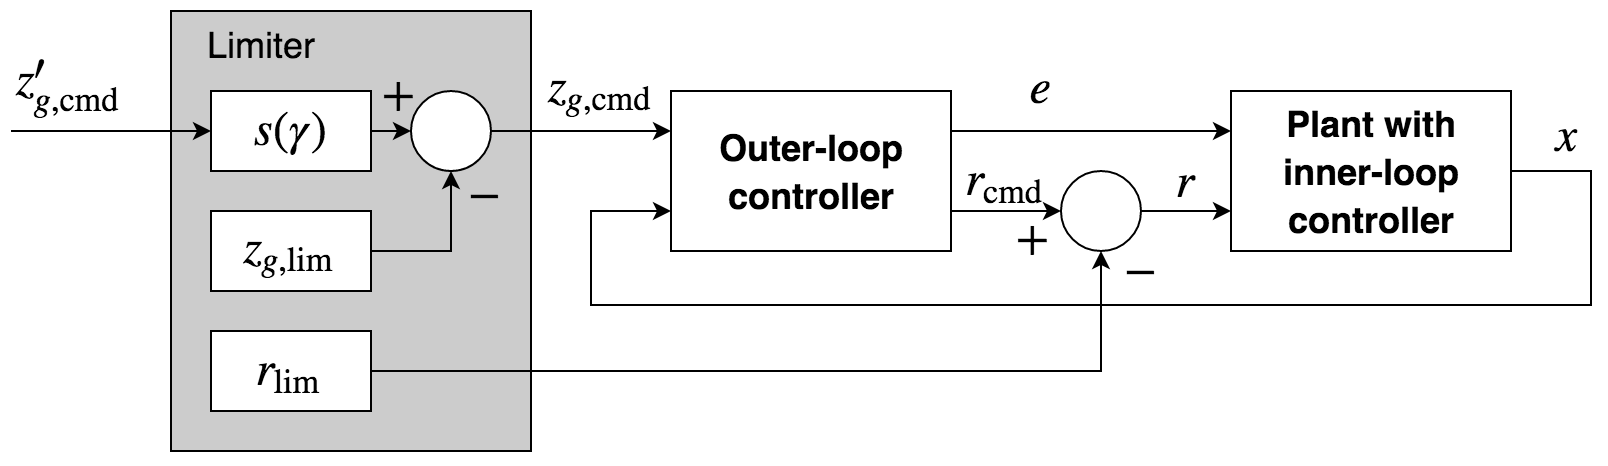
\includegraphics[width=5.5in]{\figurepath/simpleBlockWithLimiter.png}
    \vspace{-0.1in}
    \caption{Simplified outer-loop block diagram with limiter.\label{fig.simpleBlockWithLimiter}}
  \end{center}
\end{figure}

This modifies the block diagram in Figure~\ref{fig.innerAndOuterLoopDansOutputFeedback} as shown in Figure~\ref{fig.innerAndOuterLoopDansOutputFeedbackWithLimiter}.

\begin{figure}[H]
  \begin{center}
    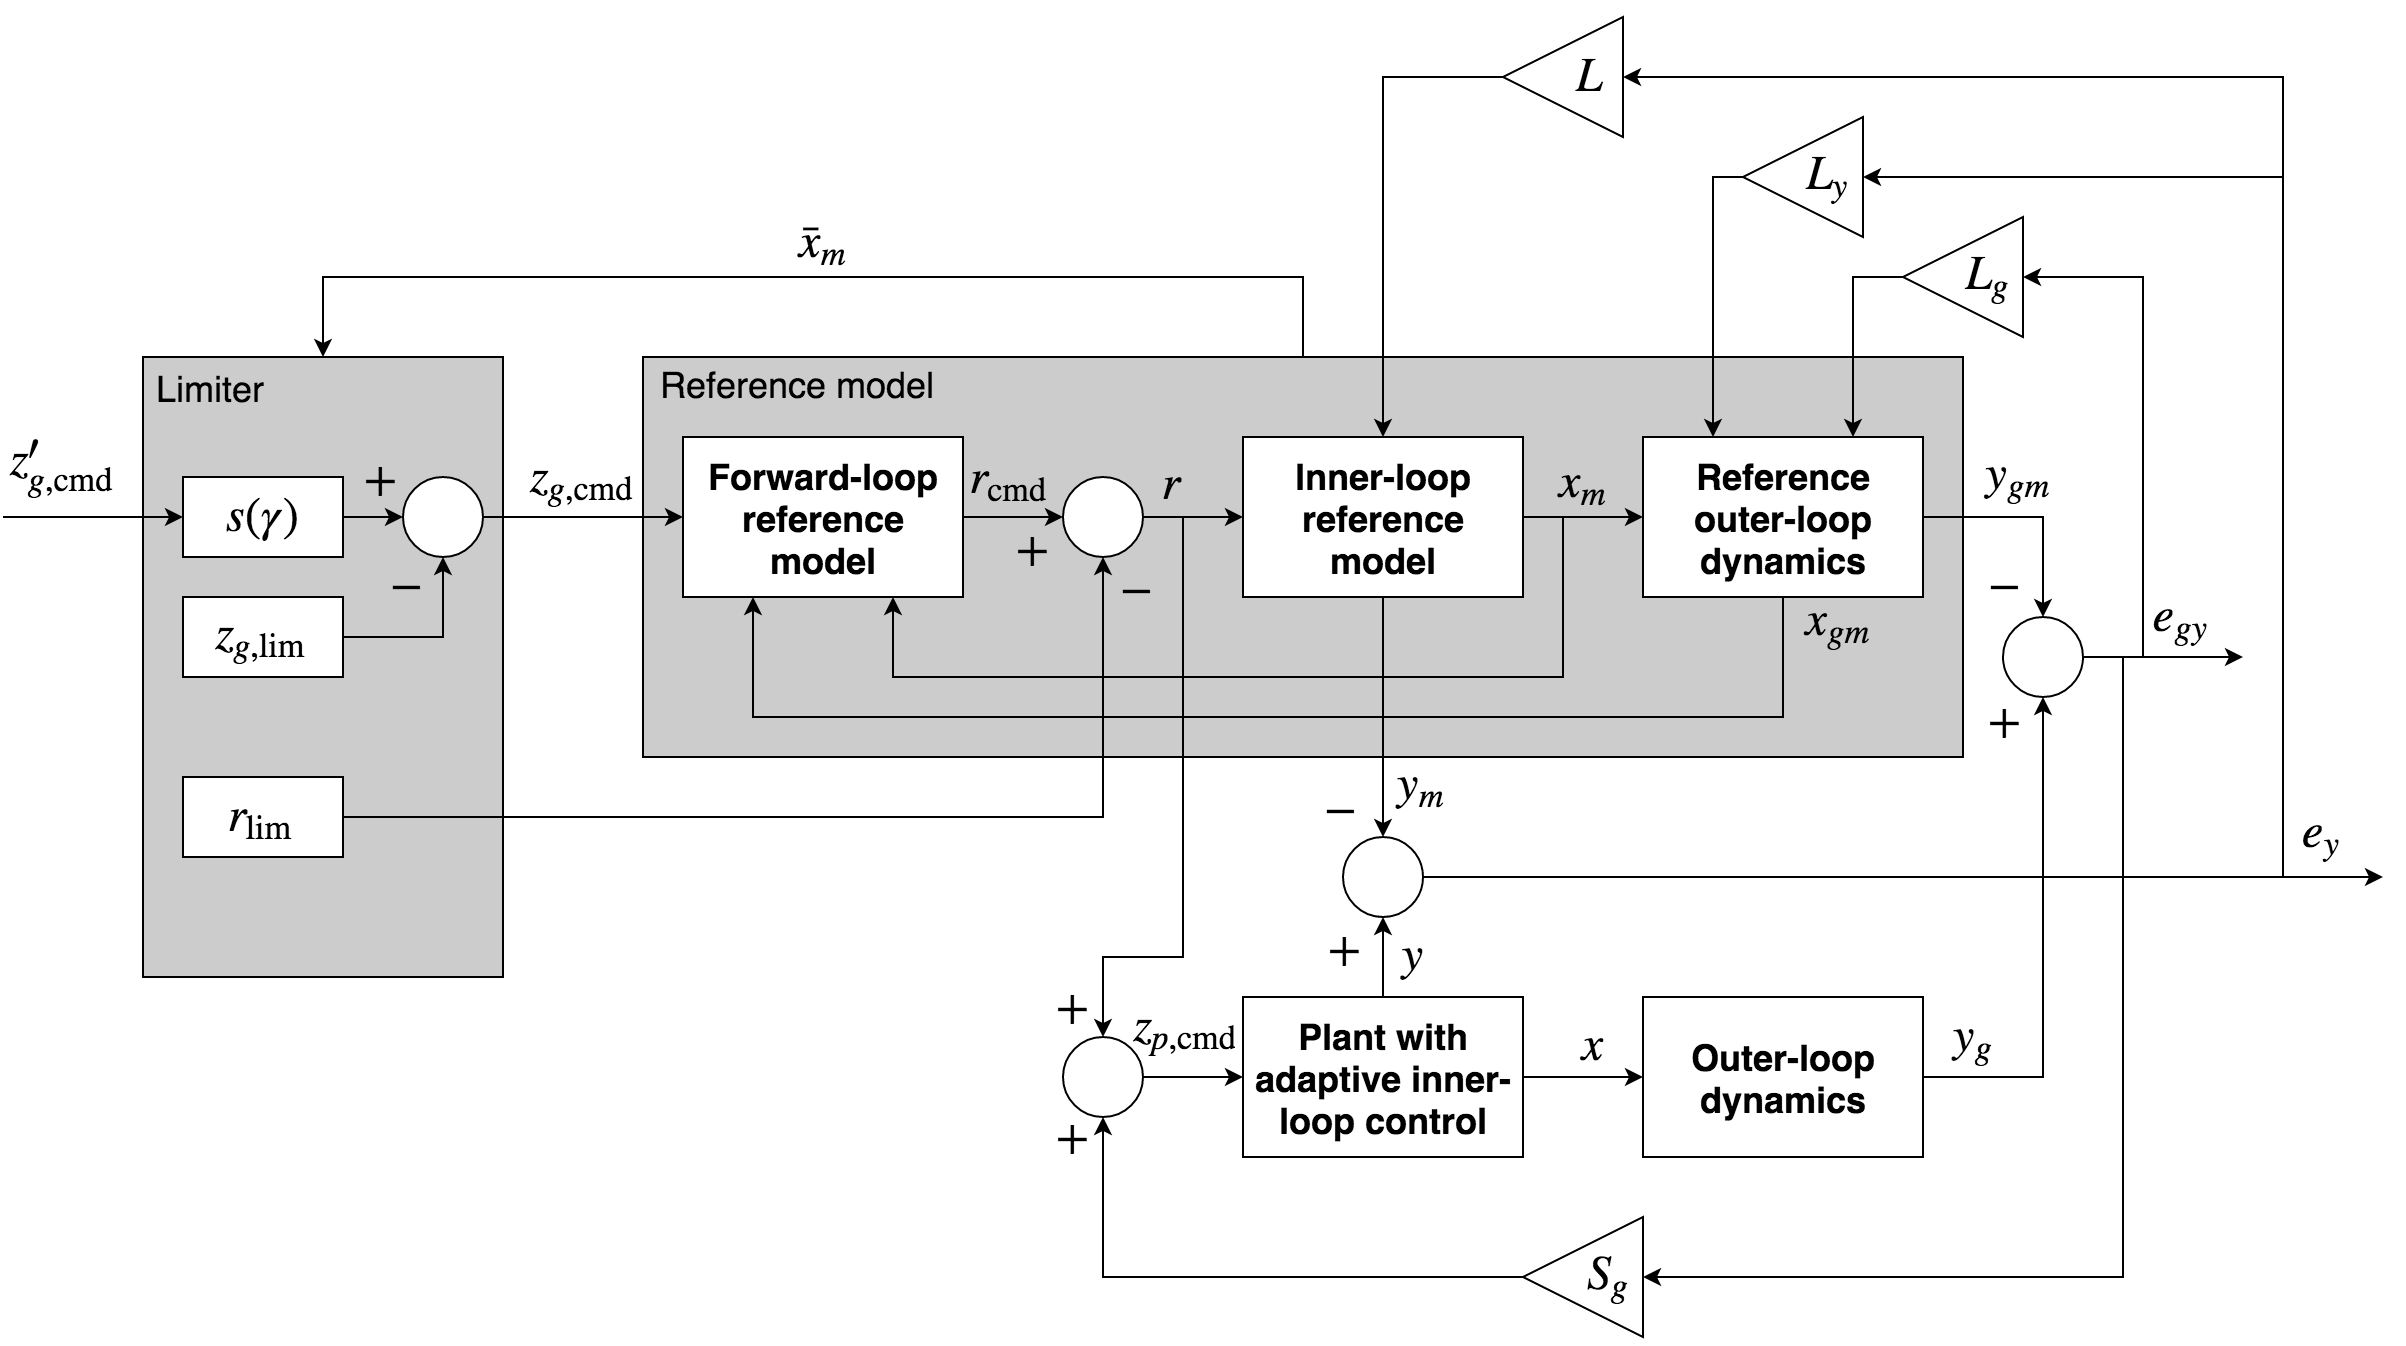
\includegraphics[width=6.5in]{\figurepath/innerAndOuterLoopDansOutputFeedbackWithLimiter.png}
    \vspace{-0.1in}
    \caption{Expanded outer-loop block diagram with limiter.\label{fig.innerAndOuterLoopDansOutputFeedbackWithLimiter}}
  \end{center}
\end{figure}

The entire reference model containing the inner-loop, the outer-loop, and forward-loop components is given in\ \eqref{eqn.xbareqnopenloop}.
When a controller as in\ \eqref{eqn.rKbar} is designed, with $\bar{K}$ as in\ \eqref{eqn.Kbar}, the entire reference model\ \eqref{eqn.xbareqnopenloop} is modified as
\begin{equation}
  \label{eqn.compactreferencemodel2}
  \begin{split}
    \dot{\bar{x}}_{m}(t)
    &=
    \bar{A}\bar{x}_{m}(t) + \bar{B}r(t) - \bar{L}_{y}e_{y}(t) - \bar{L}_{g}e_{gy}(t) + \bar{B}_{m}z_{g,\text{cmd}}^{\prime}(t) \\
    r_{\text{cmd}}(t)
    &=
    \bar{C}_{m}\bar{x}_{m}(t) \\
  \end{split}
\end{equation}
However, to facilitate command and state limiting the inner-loop command $r(t)$ and the outer-loop command $z_{g,\text{cmd}}(t)$ in\ \eqref{eqn.compactreferencemodel2} should be modified when certain reference model states become too large.
Thus inner-loop command $r(t)$ is no longer set as in\ \eqref{eqn.rrcmd} but instead as
\begin{equation}
  \label{eqn.rrcmdrlim}
  r(t) = r_{\text{cmd}}(t) - r_{\text{lim}}(t)
\end{equation}
where the inner-loop reference model command limiter $r_{\text{lim}}(t)$ is given by
\begin{equation}
  \label{eqn.rlim}
  r_{\text{lim}}(t) = -k_{r}\gamma K_{\text{lim}}\bar{x}_{m}(t)
\end{equation}
where $k_{r}\geq0$ has dimensions $k_{r}\in\mathbb{R}^{n_{ep}\times n_{ep}}$ and $K_{\text{lim}}\in\mathbb{R}^{n_{ep}\times n+n_{g}+n_{f}}$ is given by
\begin{equation}
  \label{eqn.Klim}
  K_{\text{lim}} = - R_{\text{lim}}(\bar{B}_{m}+\bar{B}k_{r})^{\top}\bar{P}
\end{equation}
where $R_{\text{lim}} = R_{\text{lim}}^{\top}\geq0$ has dimensions $R_{\text{lim}}\in\mathbb{R}^{n_{ep}\times n_{ep}}$ and $\bar{P}$ is the solution to the Lyapunov equation
\begin{equation}
  \label{eqn.LyapEqnPbar}
  \bar{A}_{m}^{\top}\bar{P}+\bar{P}\bar{A}_{m} = -\bar{Q}
\end{equation}
where $\bar{Q}=\bar{Q}^{\top}>0$.
The outer-loop command $z_{g,\text{cmd}}(t)$ is no longer selected as in\ \eqref{eqn.zgcmdzgcmdprime}, but is instead generated from the desired outer-loop command $z_{g,\text{cmd}}^{\prime}(t)$ as
\begin{equation}
  \label{eqn.zcmdlimited}
  z_{g,\text{cmd}}(t) = s\bigr(\gamma(\bar{x}_{m}(t))\bigr)z_{g,\text{cmd}}^{\prime}(t) - z_{g,\text{lim}}(t)
\end{equation}
where
\begin{equation}
  \label{eqn.sofgamma}
  s\bigr(\gamma(\bar{x}_{m}(t))\bigr) = 1-\gamma(\bar{x}_{m}(t))
\end{equation}
 and $z_{g,\text{lim}}(t)$ is given by
\begin{equation}
  \label{eqn.zglim}
  z_{g,\text{lim}}(t) = -\gamma K_{\text{lim}}\bar{x}_{m}(t)
\end{equation}
The scalar quantity $\gamma(\bar{x}_{m}(t))$ is the modulation function, which is a function of the entire reference model state $\bar{x}_{m}(t)$, and is selected such that $\gamma(\bar{x}_{m}(t))\in[0,1]$.
When $\gamma(\bar{x}_{m}(t))=0$ this corresponds to no state limiting, and when $\gamma(\bar{x}_{m}(t))=1$ this corresponds to the state limiter being fully active.
Thus, $\gamma(\bar{x}_{m}(t))$ is selected using several regions within the reference model state space such that within an inner region $\gamma(\bar{x}_{m}(t))=0$, an annulus region within which $\gamma(\bar{x}_{m}(t))$ varies between $0$ and $1$, and an outer region for which $\gamma(\bar{x}_{m}(t))=1$ as shown in Figure~\ref{fig.modulationFunction}.
See, for example the modulation function in Ref.\ \cite{lavretskywise.book.2013}.

\begin{figure}[H]
  \begin{center}
    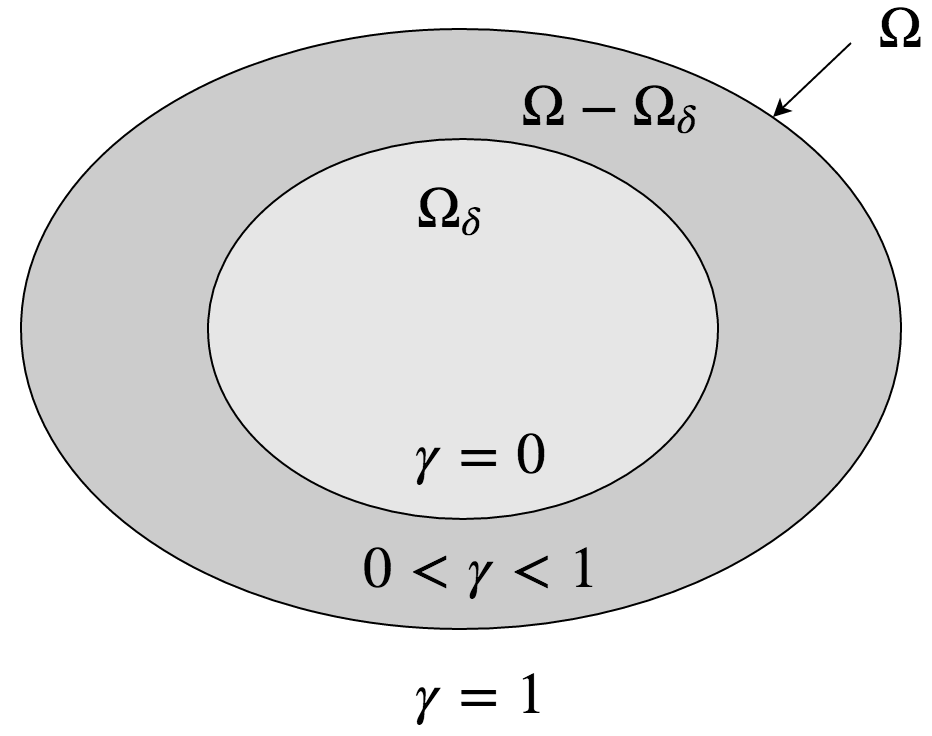
\includegraphics[width=2.5in]{\figurepath/limiterSets1.png}
    \vspace{-0.1in}
    \caption{State limiter modulation function regions from Ref.\cite{lavretsky.statelimiting.2010}\label{fig.modulationFunction}}
  \end{center}
\end{figure}

Using the outer-loop command $z_{g,\text{cmd}}(t)$ as generated by\ \eqref{eqn.zcmdlimited} into\ \eqref{eqn.compactreferencemodel2} gives
\begin{equation}
  \label{compactrefmodelwithlimiter}
  \begin{split}
    \dot{\bar{x}}_{m}(t)
    &=
    \bar{A}_{m}\bar{x}_{m}(t) + \bar{B}k_{r}\gamma(\bar{x}_{m}(t)) K_{\text{lim}}\bar{x}_{m} + \bar{B}_{m}\bigr(1-\gamma(\bar{x}_{m}(t))\bigr)z_{g,\text{cmd}}^{\prime}(t) \\
    & \qquad
    + \bar{B}_{m}\gamma(\bar{x}_{m}(t)) K_{\text{lim}}\bar{x}_{m}(t)-\bar{L}_{y}e_{y}(t) - \bar{L}_{g}e_{gy}(t) \\
    r_{\text{cmd}}(t)
    &=
    \bar{C}_{m}\bar{x}_{m}(t)
  \end{split}
\end{equation}
which can be further simplified as
\begin{equation}
  \label{compactrefmodelwithlimiter2}
  \begin{split}
    \dot{\bar{x}}_{m}(t)
    &=
    \bigr(\bar{A}_{m} + \bar{B}k_{r}\gamma(\bar{x}_{m}(t)) K_{\text{lim}} + \bar{B}_{m}\gamma(\bar{x}_{m}(t)) K_{\text{lim}}\bigr)\bar{x}_{m}(t) \\
    & \qquad
    + \bar{B}_{m}\bigr(1-\gamma(\bar{x}_{m}(t))\bigr)z_{g,\text{cmd}}^{\prime}(t) - \bar{L}_{y}e_{y}(t) - \bar{L}_{g}e_{gy}(t) \\
    r_{\text{cmd}}(t)
    &=
    \bar{C}_{m}\bar{x}_{m}(t)
  \end{split}
\end{equation}

\subsection{Stability}

Because the inner-loop reference model input $r(t)$ cancels out in the error dynamics in\ \eqref{eqn.errordynamics5}, and $z_{g,\text{cmd}}(t)$ is not present either, the state-limiter modification does not require any change to the Lyapunov function in\ \eqref{eqn.lyapfunction_2} to prove boundedness of the errors $e_{x}(t)$ and $e_{g}(t)$.
However, in the stability proof without the state limiter, the boundedness of $z_{g,\text{cmd}}(t)$, $e_{y}(t)$, and $e_{gy}(t)$ and stability of $\bar{A}_{m}$ in\ \eqref{eqn.compactreferencemodel} imply boundedness of the reference model states $x_{m}(t)$, $x_{gm}(t)$, and $x_{fm}(t)$, from which boundedness of the plant states $x(t)$ and $x_{g}(t)$ is concluded.
However, showing boundedness of the reference model states is less obvious when using the state limiter, which modifies the entire reference model dynamics in\ \eqref{eqn.compactreferencemodel} to obtain the limited reference model dynamics in\ \eqref{compactrefmodelwithlimiter}.
Thus it is necessary to ensure that with the limiting modifications the reference model state $\bar{x}_{m}(t)$ is still bounded, and global stability is still proved, as stated in the following theorem.

\begin{thm-dan}\label{thm.outerlooplimiter}
  The uncertain system in\ \eqref{eqn.wholeSystemUncertain} with inner-loop controller specified by the control law in\ \eqref{eqn.u}, update law in\ \eqref{eqn.updatelaw}, and the reference model in\ \eqref{eqn.refmodelWithBd} where $S_{1}$ and $L$ are chosen as described in Chapter~\ref{ch.innerLoop}, and the outer-loop controller specified by the outer-loop reference model in\ \eqref{eqn.refmodelouter}, forward-loop reference model component in\ \eqref{eqn.forwardloopcontroller}, with inner-loop command input $z_{p,\text{cmd}}(t)$ is prescribed by\ \eqref{eqn.zpcmd} and\ \eqref{eqn.egs}, where $r(t)$ is given by\ \eqref{compactrefmodelwithlimiter2},\ \eqref{eqn.rrcmdrlim}, and\ \eqref{eqn.rlim}, and outer-loop command generated by\ \eqref{eqn.zcmdlimited},\ \eqref{eqn.sofgamma}, and\ \eqref{eqn.zglim}, with $S_{g}$, $L_{g}$, and $L_{y}$ selected as described above, results in global stability, with $\lim_{t\rightarrow\infty}e_{x}(t)=0$ and $\lim_{t\rightarrow\infty}e_{g}(t)=0$.
\end{thm-dan}

\begin{proof-dan}
  This proof follows from the proof of Theorem~\ref{thm.outerloop} by proposing the same candidate Lyapunov function as in\ \eqref{eqn.lyapfunction_2} and differentiating to obtain\ \eqref{eqn.outerlooplyapderivative} from which it can be concluded that $e_{x}(t), \; e_{g}(t) , \;\widetilde{\Theta}(t)\in\mathcal{L}_{\infty}$.
  Bounds on $e_{x}(t)$ and $e_{g}(t)$ can be found as follows
  \begin{equation}
    \label{eqn.boundaonexandeg}
    \begin{split}
      \|e_{x}(t)\|
      & \leq
      \sqrt{\frac{V(0)}{\lambda_{\text{min}}(P_{x})}} \\
      \|e_{g}(t)\|
      & \leq
      \sqrt{\frac{V(0)}{\lambda_{\text{min}}(P_{g})}}
    \end{split}
  \end{equation}
  giving the following bounds on their respective measured output errors $e_{y}(t)$ and $e_{gy}(t)$ as
  \begin{equation}
    \label{eqn.boundaoneyandegy}
    \begin{split}
      \|e_{y}(t)\|
      & \leq
      e_{y,\text{max}}
      =
      \|C\|
      \sqrt{\frac{V(0)}{\lambda_{\text{min}}(P_{x})}} \\
      \|e_{gy}(t)\|
      & \leq
      e_{gy,\text{max}}
      =
      \|C_{g}\|
      \sqrt{\frac{V(0)}{\lambda_{\text{min}}(P_{g})}}
    \end{split}
  \end{equation}
  Propose the following additional candidate Lyapunov function to prove boundedness of the reference model state
  \begin{equation}
    \label{eqn.Lyapxmbar}
    \bar{V}\bigr(\bar{x}_{m}(t)\bigr) = \bar{x}_{m}^{\top}(t)\bar{P}\bar{x}_{m}(t)
  \end{equation}
  Differentiating\ \eqref{eqn.Lyapxmbar} gives
  \begin{equation}
    \label{eqn.Lyapxmbardot1}
    \dot{\bar{V}}\bigr(\bar{x}_{m}(t)\bigr)
    =
    \dot{\bar{x}}_{m}^{\top}(t)\bar{P}\bar{x}_{m}(t)
    + \bar{x}_{m}^{\top}(t)\bar{P}\dot{\bar{x}}_{m}(t)
  \end{equation}
  Substituting the limited reference model dynamics\ \eqref{compactrefmodelwithlimiter} into\ \eqref{eqn.Lyapxmbardot1} gives
  \begin{equation}
    \label{eqn.Lyapxmbardot2}
    \begin{split}
      \dot{\bar{V}}\bigr(\bar{x}_{m}(t)\bigr)
      &=
      \bigr(\bar{A}_{m}\bar{x}_{m}(t) + \bar{B}k_{r}\gamma(\bar{x}_{m}(t)) K_{\text{lim}}\bar{x}_{m}(t) + \bar{B}_{m}(1-\gamma(\bar{x}_{m}(t)))z_{g,\text{cmd}}^{\prime}(t) \\
      &\qquad
      +\bar{B}_{m}\gamma K_{\text{lim}}\bar{x}_{m}(t) - \bar{L}_{y}e_{y}(t) - \bar{L}_{g}e_{gy}(t)\bigr)^{\top}\bar{P}\bar{x}_{m}(t) \\
      &\qquad
      + \bar{x}_{m}^{\top}(t)\bar{P}\bigr(\bar{A}_{m}\bar{x}_{m}(t) + \bar{B}k_{r}\gamma(\bar{x}_{m}(t)) K_{\text{lim}}\bar{x}_{m}(t) + \bar{B}_{m}(1-\gamma(\bar{x}_{m}(t)))z_{g,\text{cmd}}^{\prime}(t) \\
      &\qquad
      + \bar{B}_{m}\gamma K_{\text{lim}}\bar{x}_{m}(t) - \bar{L}_{y}e_{y}(t) - \bar{L}_{g}e_{gy}(t)\bigr) \\
      &=
      \bar{x}_{m}^{\top}(t)\bigr(\bar{A}_{m}^{\top}\bar{P}+\bar{P}\bar{A}_{m}\bigr)\bar{x}_{m}(t)
      +\bar{x}_{m}^{\top}(t)K_{\text{lim}}^{\top}\gamma(\bar{x}_{m}(t)) k_{r}^{\top}\bar{B}^{\top}\bar{P}\bar{x}_{m}(t) \\
      &\qquad
      +\bar{x}_{m}^{\top}(t)\bar{P}\bar{B}k_{r}\gamma(\bar{x}_{m}(t)) K_{\text{lim}}\bar{x}_{m}(t)
      +\bar{x}_{m}^{\top}(t)K_{\text{lim}}^{\top}\gamma(\bar{x}_{m}(t))\bar{B}_{m}^{\top}\bar{P}\bar{x}_{m}(t) \\
      & \qquad
      +\bar{x}_{m}^{\top}(t)\bar{P}\bar{B}_{m}\gamma(\bar{x}_{m}(t)) K_{\text{lim}}\bar{x}_{m}(t)
      + 2\bar{x}_{m}^{\top}(t)\bar{P}\bar{B}_{m}(1-\gamma(\bar{x}_{m}(t)))z_{g,\text{cmd}}^{\prime}(t) \\
      & \qquad
      - 2\bar{x}_{m}^{\top}(t)\bar{P}(\bar{L}_{y}e_{y}(t) + \bar{L}_{g}e_{gy}(t)) \\
      &=
      \bar{x}_{m}^{\top}(t)\bigr(\bar{A}_{m}^{\top}\bar{P}+\bar{P}\bar{A}_{m}\bigr)\bar{x}_{m}(t)
      + \bar{x}_{m}^{\top}\bigr(K_{\text{lim}}^{\top}\gamma(\bar{x}_{m}(t)) k_{r}^{\top}\bar{B}^{\top}\bar{P}
      + \bar{P}\bar{B}k_{r}\gamma(\bar{x}_{m}(t)) K_{\text{lim}} \\
      &\qquad
      + K_{\text{lim}}^{\top}\gamma(\bar{x}_{m}(t))\bar{B}_{m}^{\top}\bar{P}
      +\bar{P}\bar{B}_{m}\gamma(\bar{x}_{m}(t)) K_{\text{lim}}\bigr) \bar{x}_{m}(t) \\
      & \qquad
      + 2\bar{x}_{m}^{\top}(t)\bar{P}\bar{B}_{m}\bigr(1-\gamma(\bar{x}_{m}(t))\bigr)z_{g,\text{cmd}}^{\prime}(t)
      - 2\bar{x}_{m}^{\top}(t)\bar{P}\bigr(\bar{L}_{y}e_{y}(t) + \bar{L}_{g}e_{gy}(t)\bigr) \\
      &=
      \bar{x}_{m}^{\top}(t)\bigr(\bar{A}_{m}^{\top}\bar{P}+\bar{P}\bar{A}_{m}\bigr)\bar{x}_{m}(t)
      +\bar{x}_{m}^{\top}(t)
      \bigr(K_{\text{lim}}^{\top}\gamma(\bar{x}_{m}(t)) (k_{r}^{\top}\bar{B}^{\top}+\bar{B}_{m}^{\top})\bar{P} \\
      &\qquad
      + \bar{P}(\bar{B}k_{r}+\bar{B}_{m})\gamma(\bar{x}_{m}(t)) K_{\text{lim}}\bigr) \bar{x}_{m}(t) \\
      & \qquad
      + 2\bar{x}_{m}^{\top}(t)\bar{P}\bar{B}_{m}\bigr(1-\gamma(\bar{x}_{m}(t))\bigr)z_{g,\text{cmd}}^{\prime}(t)
      - 2\bar{x}_{m}^{\top}(t)\bar{P}\bigr(\bar{L}_{y}e_{y}(t)+\bar{L}_{g}e_{gy}(t)\bigr) \\
    \end{split}
  \end{equation}
  Using $K_{\text{lim}}$ as in\ \eqref{eqn.Klim} where $\bar{P}$ is the solution to the Lyapunov equation\ \eqref{eqn.LyapEqnPbar}, the derivative in\ \eqref{eqn.Lyapxmbardot2} becomes
  \begin{equation}
    \label{eqn.Lyapxmbardot3}
    \begin{split}
      \dot{\bar{V}}\bigr(\bar{x}_{m}(t)\bigr)
      &=
      \bar{x}_{m}^{\top}(t)\bigr(\bar{A}_{m}^{\top}\bar{P}+\bar{P}\bar{A}_{m}\bigr)\bar{x}_{m}(t)
      -
      \bar{x}_{m}^{\top}(t)
      \bigr(
      \bar{P}(\bar{B}_{m}+\bar{B}k_{r})R_{\text{lim}}^{\top}\gamma(\bar{x}_{m}(t)) (k_{r}^{\top}\bar{B}^{\top}+\bar{B}_{m}^{\top})\bar{P} \\
      & \qquad
      +\bar{P}(\bar{B}k_{r}+\bar{B}_{m})R_{\text{lim}}(\bar{B}_{m}+\bar{B}k_{r})^{\top}\bar{P}
      \bigr) \bar{x}_{m}(t) \\
      & \qquad
      + 2\bar{x}_{m}^{\top}(t)\bar{P}\bar{B}_{m}\bigr(1-\gamma(\bar{x}_{m}(t))\bigr)z_{g,\text{cmd}}^{\prime}(t)
      - 2\bar{x}_{m}^{\top}(t)\bar{P}\bigr(\bar{L}_{y}e_{y}(t)+\bar{L}_{g}e_{gy}(t)\bigr) \\
      &=
      \bar{x}_{m}^{\top}(t)\bigr(\bar{A}_{m}^{\top}\bar{P}+\bar{P}\bar{A}_{m}\bigr)\bar{x}_{m}(t) \\
      &\qquad
      -\bar{x}_{m}^{\top}(t)
      \bigr(
      2\bar{P}(\bar{B}_{m}+\bar{B}k_{r})R_{\text{lim}}^{\top}\gamma(\bar{x}_{m}(t)) (k_{r}^{\top}\bar{B}^{\top}+\bar{B}_{m}^{\top})\bar{P}
      \bigr) \bar{x}_{m}(t) \\
      & \qquad
      + 2\bar{x}_{m}^{\top}(t)\bar{P}\bar{B}_{m}\bigr(1-\gamma(\bar{x}_{m}(t))\bigr)z_{g,\text{cmd}}^{\prime}(t)
      - 2\bar{x}_{m}^{\top}(t)\bar{P}\bigr(\bar{L}_{y}e_{y}(t)+\bar{L}_{g}e_{gy}(t)\bigr) \\
    \end{split}
  \end{equation}
  Using $\bar{Q}$ from\ \eqref{eqn.LyapEqnPbar} and defining the following
  \begin{equation}
    \label{eqn.qbarlim}
    \bar{Q}_{\rm{\lim}}(\gamma)
    =
    2\bar{P}(\bar{B}_{m}+\bar{B}k_{r})R_{\text{lim}}^{\top}\gamma (k_{r}^{\top}\bar{B}^{\top}+\bar{B}_{m}^{\top})\bar{P}
    \geq
    0
  \end{equation}
  allowing\ \eqref{eqn.Lyapxmbardot3} to be rewritten as
  \begin{equation}
    \label{eqn.vbardot}
    \begin{split}
      \dot{\bar{V}}\bigr(\bar{x}_{m}(t)\bigr)
      &=
      -\bar{x}_{m}^{\top}(t)(\bar{Q}+\bar{Q}_{\rm{\lim}}(\gamma))\bar{x}_{m}(t) + 2\bar{x}_{m}^{\top}(t)\bar{P}\bar{B}_{m}(1-\gamma)z_{g,\text{cmd}}^{\prime}(t) \\
      &\qquad
      - 2\bar{x}_{m}^{\top}(t)\bar{P}\bigr(\bar{L}_{y}e_{y}(t)+\bar{L}_{g}e_{gy}(t)\bigr) \\
      &=
      -\bar{x}_{m}^{\top}(\bar{Q}+\bar{Q}_{\rm{\lim}}(\gamma))\bar{x}_{m}(t) + 2\bar{x}_{m}^{\top}(t)\bar{P}\bigr(\bar{B}_{m}(1-\gamma)z_{g,\text{cmd}}^{\prime}(t) - \bar{L}_{y}e_{y}(t) - \bar{L}_{g}e_{gy}(t)\bigr)
    \end{split}
  \end{equation}
  Note that the bounds on $e_{y}(t)$ and $e_{gy}(t)$ in\ \eqref{eqn.boundaoneyandegy} are independent of $\bar{x}_{m}(t)$.
  Eq.\ \eqref{eqn.vbardot} contains a negative quadratic term in $\bar{x}_{m}(t)$, and a sign indefinite term which is linear in $\bar{x}_{m}(t)$.
  Thus, for sufficiently large $\bar{x}_{m}(t)$, the derivative $\dot{\bar{V}}\bigr(x_{m}(t)\bigr)$ in\ \eqref{eqn.vbardot} becomes strictly negative.
  This is quantified precisely by the following statement: $\dot{\bar{V}}\bigr(\bar{x}_{m}(t)\bigr)<0$ outside the compact set
  \begin{equation}
    \label{eqn.limiterCompactSet}
    E_{\delta}=
    \biggr\{
    \bar{x}_{m}(t)\in\mathbb{R}^{n} \; : \;
    \|\bar{x}_{m}(t)\|
    \leq
    \frac{2\lambda_{\text{max}}(\bar{P})\bigr(
    \|\bar{B}_{m}\|(1-\gamma)z_{g,\text{cmd,max}}^{\prime}+
    \|\bar{L}_{y}\|e_{y,\text{max}}+\|\bar{L}_{g}\|e_{gy,\text{max}}
    \bigr)}{\lambda_{\text{min}}(\bar{Q}+\bar{Q}_{\text{lim}}(\gamma))}
    \biggr\}
  \end{equation}
  for all $\gamma(\bar{x}_{m}(t))\in[0,1]$.
  Thus the entire reference model state $\bar{x}_{m}(t)$ is bounded\ \cite{narendra.stable.2005} which, with the boundedness of the errors $e_{x}(t)$ and $e_{g}(t)$, implies that $x(t),\;x_{g}(t)\in\mathcal{L}_{\infty}$.
  With $e_{x}(t),\;e_{g}(t),\;x_{m}(t),\;\widetilde{\Theta}\in\mathcal{L}_{\infty}$, and the the error dynamics in\ \eqref{eqn.innerAndOuterLoopErrorDynamics2}, this implies that $\dot{e}_{x}(t), \; \dot{e}_{g}(t)\in\mathcal{L}_{\infty}$.
  Finally, $\int_{0}^{t}\dot{V}(\tau)d\tau=V(t)-V(0)$ and since $V(t)$ is non-increasing and positive definite, $V(0)-V(t)\leq V(0)$.
  This gives $-\int_{0}^{t}\dot{V}(\tau)d\tau\leq V(0)$.
  Substituting in the expression for $\dot{V}= - e_{x}^{\top}(t)Q_{x}e_{x}(t) - e_{g}^{\top}(t)Q_{g}e_{g}(t)$ gives $\int_{0}^{t}e_{x}(\tau)^{\top}Q_{x}e_{x}(\tau) + e_{g}(\tau)^{\top}Q_{g}e_{g}(\tau)d\tau\leq V(0)$ and in turn that $e_{x}(t),\;e_{g}(t)\in\mathcal{L}_{2}$.
  With this, it can be concluded using Barbalat's Lemma\ \cite{narendra.stable.2005} that $\lim_{t\rightarrow\infty}e_{x}(t)=0$ and $\lim_{t\rightarrow\infty}e_{g}(t)=0$.
\end{proof-dan}

Theorem~\ref{thm.outerlooplimiter} proves stability of the closed-loop system with state limiter, with asymptotic tracking of the reference model states $x_{m}(t)$ and $x_{gm}(t)$ by the plant states $x(t)$ and $x_{g}(t)$, respectively.
In the absence of the state limiter, satisfaction of the control goal of outer-loop command tracking was discussed in Corollary~\ref{cor.zgcmdtracking}.
When using the state limiter, Theorem~\ref{thm.outerloop}, like Theorem~\ref{thm.outerlooplimiter}, provided $z_{g}(t)\rightarrow z_{gm}(t)$ as $t\rightarrow\infty$.
However, without the limiter, the reference model in\ \eqref{eqn.compactreferencemodel} was selected so that $z_{gm}(t)$ was a filtered version of the outer-loop command, so that asymptotic tracking of constant commands was achieved, as given by Corollary~\ref{cor.zgcmdtracking}.
When using the limiter, the reference model dynamics in\ \eqref{compactrefmodelwithlimiter} are modified such that $z_{gm}(t)$ is no longer simply a filtered version of the outer-loop command $z_{g,\text{cmd}}^{\prime}(t)$.
Thus asymptotic tracking of $z_{g,\text{cmd}}^{\prime}(t)$ by $z_{g}(t)$ doesn't hold in general, due to the scaling of the outer-loop command by the limiter.
However, if a desired outer-loop command $z_{g,\text{cmd}}^{\prime}(t)$ is given such that the limiter is inactive and $\gamma\bigr(\bar{x}_{m}(t)\bigr)=0$, the same conclusion as in Corollary~\ref{cor.zgcmdtracking} can be made, with $z_{g,\text{cmd}}(t) = z_{g,\text{cmd}}^{\prime}(t)$.
This statement is formalized in the following corollary to Theorem~\ref{thm.outerlooplimiter}.

\begin{cor-dan}\label{cor.notForcingLimiting}
  For all piecewise constant outer-loop command inputs $z_{g,\text{\rm{cmd}}}^{\prime}(t)$ which satisfy $\|z_{g,\text{\rm{cmd}}}^{\prime}(t)\|_{\infty}\leq z_{g,\text{\rm{cmd,max}}}^{\prime}$, the outer-loop regulated output $z_{g}(t)$ tracks $z_{g,\text{\rm{cmd}}}^{\prime}(t)$ asymptotically, where $z_{g,\text{\rm{cmd,max}}}^{\prime}$ is given by
  \begin{equation}
    \label{eqn.zgcmdprimemax}
    z_{g,\text{\rm{cmd,max}}}^{\prime}=
    \frac{\bar{x}_{m,\text{\rm{max}}}}{\|h_{m}\|_{1}}
  \end{equation}
  where $h_{m}$ is the impulse response of the nominal reference model, given by\ \eqref{compactrefmodelwithlimiter2} with $\gamma(\bar{x}_{m}(t))=0$, $\bar{L}_{y}=0$ and $\bar{L}_{g}=0$, and $\bar{x}_{m,\text{\rm{max}}}=\text{\rm{max}}_{\bar{x}_{m}(t)\in\Omega_{\delta}}\|\bar{x}_{m}(t)\|$.
\end{cor-dan}

\begin{proof-dan}
  For all $\bar{x}_{m}(t)\in\Omega_{\delta}$ the state limiter is inactive, and the evolution of the reference model state $\bar{x}_{m}(t)$ is governed by\ \eqref{compactrefmodelwithlimiter2} with $\gamma(\bar{x}_{m}(t))=0$, while $e_{y}(t)$ and $e_{gy}(t)$ tend to zero asymptotically.
  Thus, the reference model state $\bar{x}_{m}(t)$ ultimately depends only on the command input $z_{g,\text{cmd}}^{\prime}(t)$.
  The following bound on the reference model state holds, where $h_{m}$ is the impulse response of the nominal reference model,\ \eqref{compactrefmodelwithlimiter2} with $\gamma(\bar{x}_{m}(t))=0$.
  \begin{equation*}
    \|\bar{x}_{m}(t)\|_{\infty}=\bar{x}_{m,\text{max}} \leq \|h_{m}\|_{1}\|z_{g,\text{cmd}}^{\prime}(t)\|_{\infty}
  \end{equation*}
  From this, the bound on the command input can be found as in\ \eqref{eqn.zgcmdprimemax} that ensures the reference model state $\bar{x}_{m}(t)\in\Omega_{\delta}$, thus not invoking the state limiter, and providing the tracking properties given in Corollary~\ref{cor.zgcmdtracking}.
\end{proof-dan}

\begin{rem-dan}
  Corollary~\ref{cor.notForcingLimiting} states that if the desired outer-loop command $z_{g,\text{cmd}}^{\prime}(t)$ is such that the system is not driven to enter the limiting region, that the limiter will not impact tracking performance of the system.
  This is due to the fact that the convergence of the tracking errors $e_{y}(t)$ and $e_{gy}(t)$ to zero is obtained regardless of whether the limiter is invoked or not.
  In other words, as these errors tend to zero, only the desired outer-loop command $z_{g,\text{cmd}}^{\prime}(t)$ can drive the reference model state $\bar{x}_{m}(t)$ out of $\Omega_{\delta}$, as governed by\ \eqref{eqn.compactreferencemodel}.
  Thus, if the desired outer-loop command is such that it does not force $\bar{x}_{m}(t)$ outside of $\Omega_{\delta}$, the limiter will become inactive.
  Corollary~\ref{cor.notForcingLimiting} then finds the maximum value of $z_{g,\text{cmd}}^{\prime}(t)$ such that $\bar{x}_{m}(t)\in\Omega_{\delta}$ using the impulse response of the reference model.
\end{rem-dan}

\begin{rem-dan}
  The benefits of the state limiter are apparent from the compact set in\ \eqref{eqn.limiterCompactSet} outside of which $\dot{\bar{V}}(\bar{x}_{m}(t))<0$.
  The size of $E_{\delta}$ monotonically decreases in size as $\gamma(\bar{x}_{m}(t))$ increases, hence shrinking the bound on $\bar{x}_{m}(t)$ when the limiter is invoked, versus without the limiter.
\end{rem-dan}

\subsubsection{Degrees of Freedom}

The limiter described above has several degrees of freedom which can be chosen by the designer to achieve the desired performance.
These degrees of freedom are the gains $k_{r}$, $R_{\text{lim}}$, $\bar{Q}$, and the modulation function $\gamma(\bar{x}_{m}(t))$ and the corresponding sets $\Omega$ and $\Omega_{\delta}$.
The limiter components $r_{\text{lim}}(t)$ and $z_{g,\text{lim}}(t)$ enter through the input matrices $\bar{B}$ and $\bar{B}_{m}$, respectively, of the reference model in\ \eqref{eqn.compactreferencemodel2}.
The matrix $R_{\text{lim}}$ scales $K_{\text{lim}}$ in\ \eqref{eqn.Klim}, which is the gain used in both of the limiting components $r_{\text{lim}}(t)$ and $z_{g,\text{lim}}(t)$, whereas $k_{r}$ scales only $r_{\text{lim}}(t)$.
Thus, by adjusting $R_{\text{lim}}$ and $k_{r}$, the relative influence of the limiter through $\bar{B}$ and $\bar{B}_{m}$ can be changed.
This alters the the effective reference model matrix in\ \eqref{compactrefmodelwithlimiter2} when the limiter becomes active, and thus $\bar{Q}_{\rm{\lim}}(\gamma(\bar{x}_{m}(t)))$ in\ \eqref{eqn.qbarlim}.
This, along with the matrix $\bar{Q}$, alters the region outside of which $\dot{\bar{V}}<0$, and thus affects the time response of the system when the state limiter is active.
With $k_{r}=0$ and $R_{\text{lim}}=0$ the limiter would still be stable, however the only adjustment would come through the reduction of the outer-loop command $z_{g,\text{cmd}}^{\prime}(t)$ in\ \eqref{eqn.vbardot}.
The modulation function $\gamma(\bar{x}_{m}(t))$ simply defines based on $\bar{x}_{m}$ when the limiter becomes active, and can be selected so as to depend on the various elements of $\bar{x}_{m}(t)$ as desired.

\subsection{Complete Controller Summary with Limiter}

The entire system closed-loop system, consisting of the plant and controller, can be summarized with the following set of equations.
The uncertain plant\ \eqref{eqn.uncsystemWithBd}, the outer-loop dynamics\ \eqref{eqn.outerLoopDynamics}, the inner-loop reference model\ \eqref{eqn.refmodelWithBd}, outer-loop reference model\ \eqref{eqn.refmodelouter}, forward-loop reference model component\eqref{eqn.forwardloopcontroller}, with inner-loop command input prescribed by\ \eqref{eqn.rrcmdrlim},\ \eqref{eqn.zpcmd} and\ \eqref{eqn.egs},\ \eqref{eqn.rlim} and outer-loop command generated by\ \eqref{eqn.zcmdlimited},\ \eqref{eqn.sofgamma}, and\ \eqref{eqn.zglim}, control law\eqref{eqn.u}, inner-loop command input\ \eqref{eqn.zpcmd} and\ \eqref{eqn.egs}, and update law\ \eqref{eqn.updatelaw} together are summarized as follows.

\begin{equation*}
  \begin{aligned}
    \textbf{Plant:}
    && \dot{x}(t) &= Ax(t) + B\bigr(\Lambda u(t) + \Psi^{\top}x(t)\bigr) + B_{\text{cmd}}z_{p,\text{cmd}}(t) + B_{d}x_{g}(t) \\
    && \dot{x}_{g}(t) &= A_{g}x_{g}(t) + B_{g}x(t) \\
    \textbf{Reference model:}
    && \dot{x}_{m}(t) &= A_{m}x_{m}(t) + B_{\text{cmd}}r(t) - Le_{y}(t) + B_{d}x_{gm}(t) \\
    && \dot{x}_{gm}(t) &= B_{g}x_{m}(t) + A_{g}x_{gm}(t) - L_{y}e_{y}(t) - L_{g}e_{gy}(t) \\
    && \dot{x}_{fm}(t) &= B_{f3}x_{m}(t) + B_{f2}x_{gm}(t) + A_{fm}x_{fm}(t) + B_{f1}z_{g,\text{cmd}}(t) \\
    \textbf{Command:}
    && r_{\text{cmd}}(t) &= C_{fm}x_{fm}(t) + D_{f1}z_{g,\text{cmd}}(t) + D_{f2}x_{gm}(t) + D_{f3} x_{m}(t) \\
    && r(t) &= r_{\text{cmd}}(t) - r_{\text{lim}}(t) \\
    && r_{\text{lim}}(t) &= -k_{r}\gamma\bigr(\bar{x}_{m}(t)\bigr) K_{\text{lim}}\bar{x}_{m}(t) \\
    && z_{g,\text{cmd}}(t) &= s(\gamma)z_{g,\text{cmd}}^{\prime}(t) - z_{g,\text{lim}}(t) \\
    && z_{p,\text{cmd}}(t) &= r(t) + S_{g}e_{gy}(t) \\
    \textbf{Errors:}
    && e_{y}(t) &= C\bigr(x(t)-x_{m}(t)\bigr) \\
    && e_{gy}(t) &= C_{g}\bigr(x_{g}(t) - x_{gm}(t)\bigr) \\
    \textbf{Control:}
    && u(t) &= \bigr(K_{x}+\Theta(t)\bigr)^{\top}x_{m}(t) \\
    && \dot{\Theta}(t) &= -\Gamma x_{m}(t)\bigr(S_{1}e_{y}(t)\bigr)^{\top}\text{sgn}(\Lambda) \\
  \end{aligned}
\end{equation*}

\section{Numerical Examples}\label{sec.outerLoopNumericalExample}

\subsection{Example 1: Inverted Pendulum Cart}

The inverted pendulum on a cart example from Section~\ref{sec.innerLoopNumericalExample} is continued here.
In the first part of this example, the inner-loop adaptive controller was used to accommodate uncertainties in the viscous damping coefficients and force input, and enforced tracking of the commanded cart velocity.
The example is continued here using the plant with this adaptive inner-loop, and the outer-loop controller prescribe the necessary cart velocity command so as to track pendulum position commands.
The pendulum position was selected as the output so as to satisfy the rank condition in\ \eqref{eqn.gsvdmatrixfullrank}, requiring that the outer-loop output supply sufficient information about the system beyond simply an integration of the inner-loop output.
This is essentially the statement that if the entire system as in the form\ \eqref{eqn.wholeSystemUncertain} is not observable through only $y_{p}(t)$, that integrating this output will not make it observable.

\begin{figure}[H]
  \begin{center}
    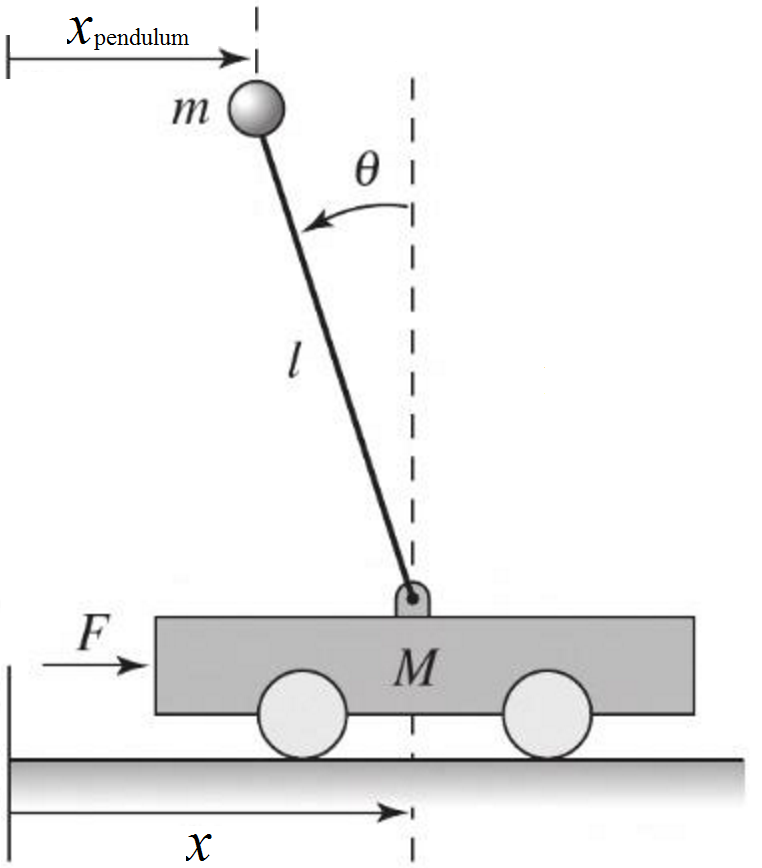
\includegraphics[width=2.8in]{\figurepath/pendulumCart.png}
    \vspace{-0.1in}
    \caption{Inverted pendulum on cart from Ref.\ \cite{astrom.feedbackintro.2010}.\label{fig.pendulumCart}}
  \end{center}
\end{figure}

The pendulum cart dynamics in\ \eqref{eqn.pendulumCartWhole} were partitioned into the inner-loop dynamics in\ \eqref{eqn.pendulumCartInnerLoop} and the outer-loop dynamics in the form of\ \eqref{eqn.outerLoopDynamics} given in\ \eqref{eqn.pendulumCartOuterLoop} below
\begin{equation}
  \label{eqn.pendulumCartOuterLoop}
  \begin{split}
    \begin{bmatrix}
      \dot{\theta} \\
      \dot{x}
    \end{bmatrix}
    &=
    \begin{bmatrix}
      0 & 0 \\
      0 & 0 \\
    \end{bmatrix}
    \begin{bmatrix}
      \theta \\
      x
    \end{bmatrix}
    +
    \begin{bmatrix}
      1 & 0 \\
      0 & 1 \\
    \end{bmatrix}
    \begin{bmatrix}
      \dot{\theta} \\
      \dot{x} \\
    \end{bmatrix} \\
    x_{\text{pendulum}}
    &=
    \begin{bmatrix}
      l & 1
    \end{bmatrix}
    \begin{bmatrix}
      \theta \\
      x
    \end{bmatrix}
  \end{split}
\end{equation}
The matrix $B_{gd}$ which couples outer-loop kinematics into the inner-loop dynamics is given by the following
\begin{equation*}
  B_{gd}
  =
  \begin{bmatrix}
    \frac{M_{t}mgl}{\mu} & 0 \\
    \frac{m^{2}g^{2}l}{\mu} & 0
  \end{bmatrix}
\end{equation*}
Using the numerical values for the pendulum given in Section\ref{sec.innerLoopNumericalExample}, the relevant matrices are given by
\begin{equation*}
  A_{g} =
  \begin{bmatrix}
    0 & 0 \\
    0 & 0
  \end{bmatrix}
  \qquad
  B_{gp} =
  \begin{bmatrix}
    1 & 0 \\
    0 & 1
  \end{bmatrix}
  \qquad
  C_{g} =
  \begin{bmatrix}
    1 \\
    1
  \end{bmatrix}^{\top}
  \qquad
  C_{gz} =
  \begin{bmatrix}
    1 \\
    1
  \end{bmatrix}^{\top}
  \qquad
  B_{gd} =
  \begin{bmatrix}
    19.6 & 0 \\
    96.04 & 0
  \end{bmatrix}^{\top}
\end{equation*}
The forward-loop reference model was designed using integral action on the regulated output as in\ \eqref{eqn.rKbar} using the following weighting matrices
\begin{equation*}
  \begin{split}
    Q_{\text{lqr}}
    &=
    \text{diag}\bigr(
    \begin{bmatrix}
      0 & 0 & 0 & 0 & 0 & 1
    \end{bmatrix}
    \bigr) \\
    R_{\text{lqr}}
    &=
    0.01
  \end{split}
\end{equation*}
Using the outer-loop design procedure summarized in Section~\ref{sec.outerLoopDesignProcedureSummary}, $P_{g}$ was calculated as in\ \eqref{eqn.Pg} using $P$ calculated as in\ \eqref{eqn.P} and $X_{D}$, where $P_{\Lambda}$ in\ \eqref{eqn.P}, and $X_{D}$ was selected as
\begin{equation*}
  X_{D}
  =
  \begin{bmatrix}
    1.0001 & 0.0086621 \\
    0.0086621 & 1
  \end{bmatrix}
  \qquad
  P_{\Lambda}
  =
  \begin{bmatrix}
    0.025 & 0 \\
    0 & 0.025
  \end{bmatrix}
\end{equation*}
With the resulting $P_{g}$, $S_{g}$ was determined using\ \eqref{eqn.SgCaseI}, and $L_{g}$ obtained numerically satisfying\ \eqref{eqn.condition4a}.
Finally $L_{y}$ was computed using\ \eqref{eqn.Ly} thus completing the outer-loop control design.

The following plot in Fig.~\ref{fig.outerLoopPendulumCart} shows the response of the closed-loop system to track pendulum position commands, when subject to the same uncertainties described in Section\ref{sec.innerLoopNumericalExample}.
As in the first example, the plot shows the baseline controller applied to the nominal plant until $t=10$ seconds when the uncertainty is introduced.
At $t=30$ seconds the adaptive controller is turned on.
As in the inner-loop example, the adaptive element ensures stability in the presence of the uncertainty, and outer-loop command tracking is provided.
However, there are significant oscillations in the response due to the uncertainty, with the pendulum reaching angular velocities of 200 deg/s.
Fig.~\ref{fig.outerLoopStateLimiterPendulumCart} shows the response of the same system, but with the limiter used to limit the angular velocity of the pendulum to within 80 deg/s.

\newpage
\begin{figure}[H]
  \hspace{-0.25in}
  \noindent\makebox[7.0in]{%
  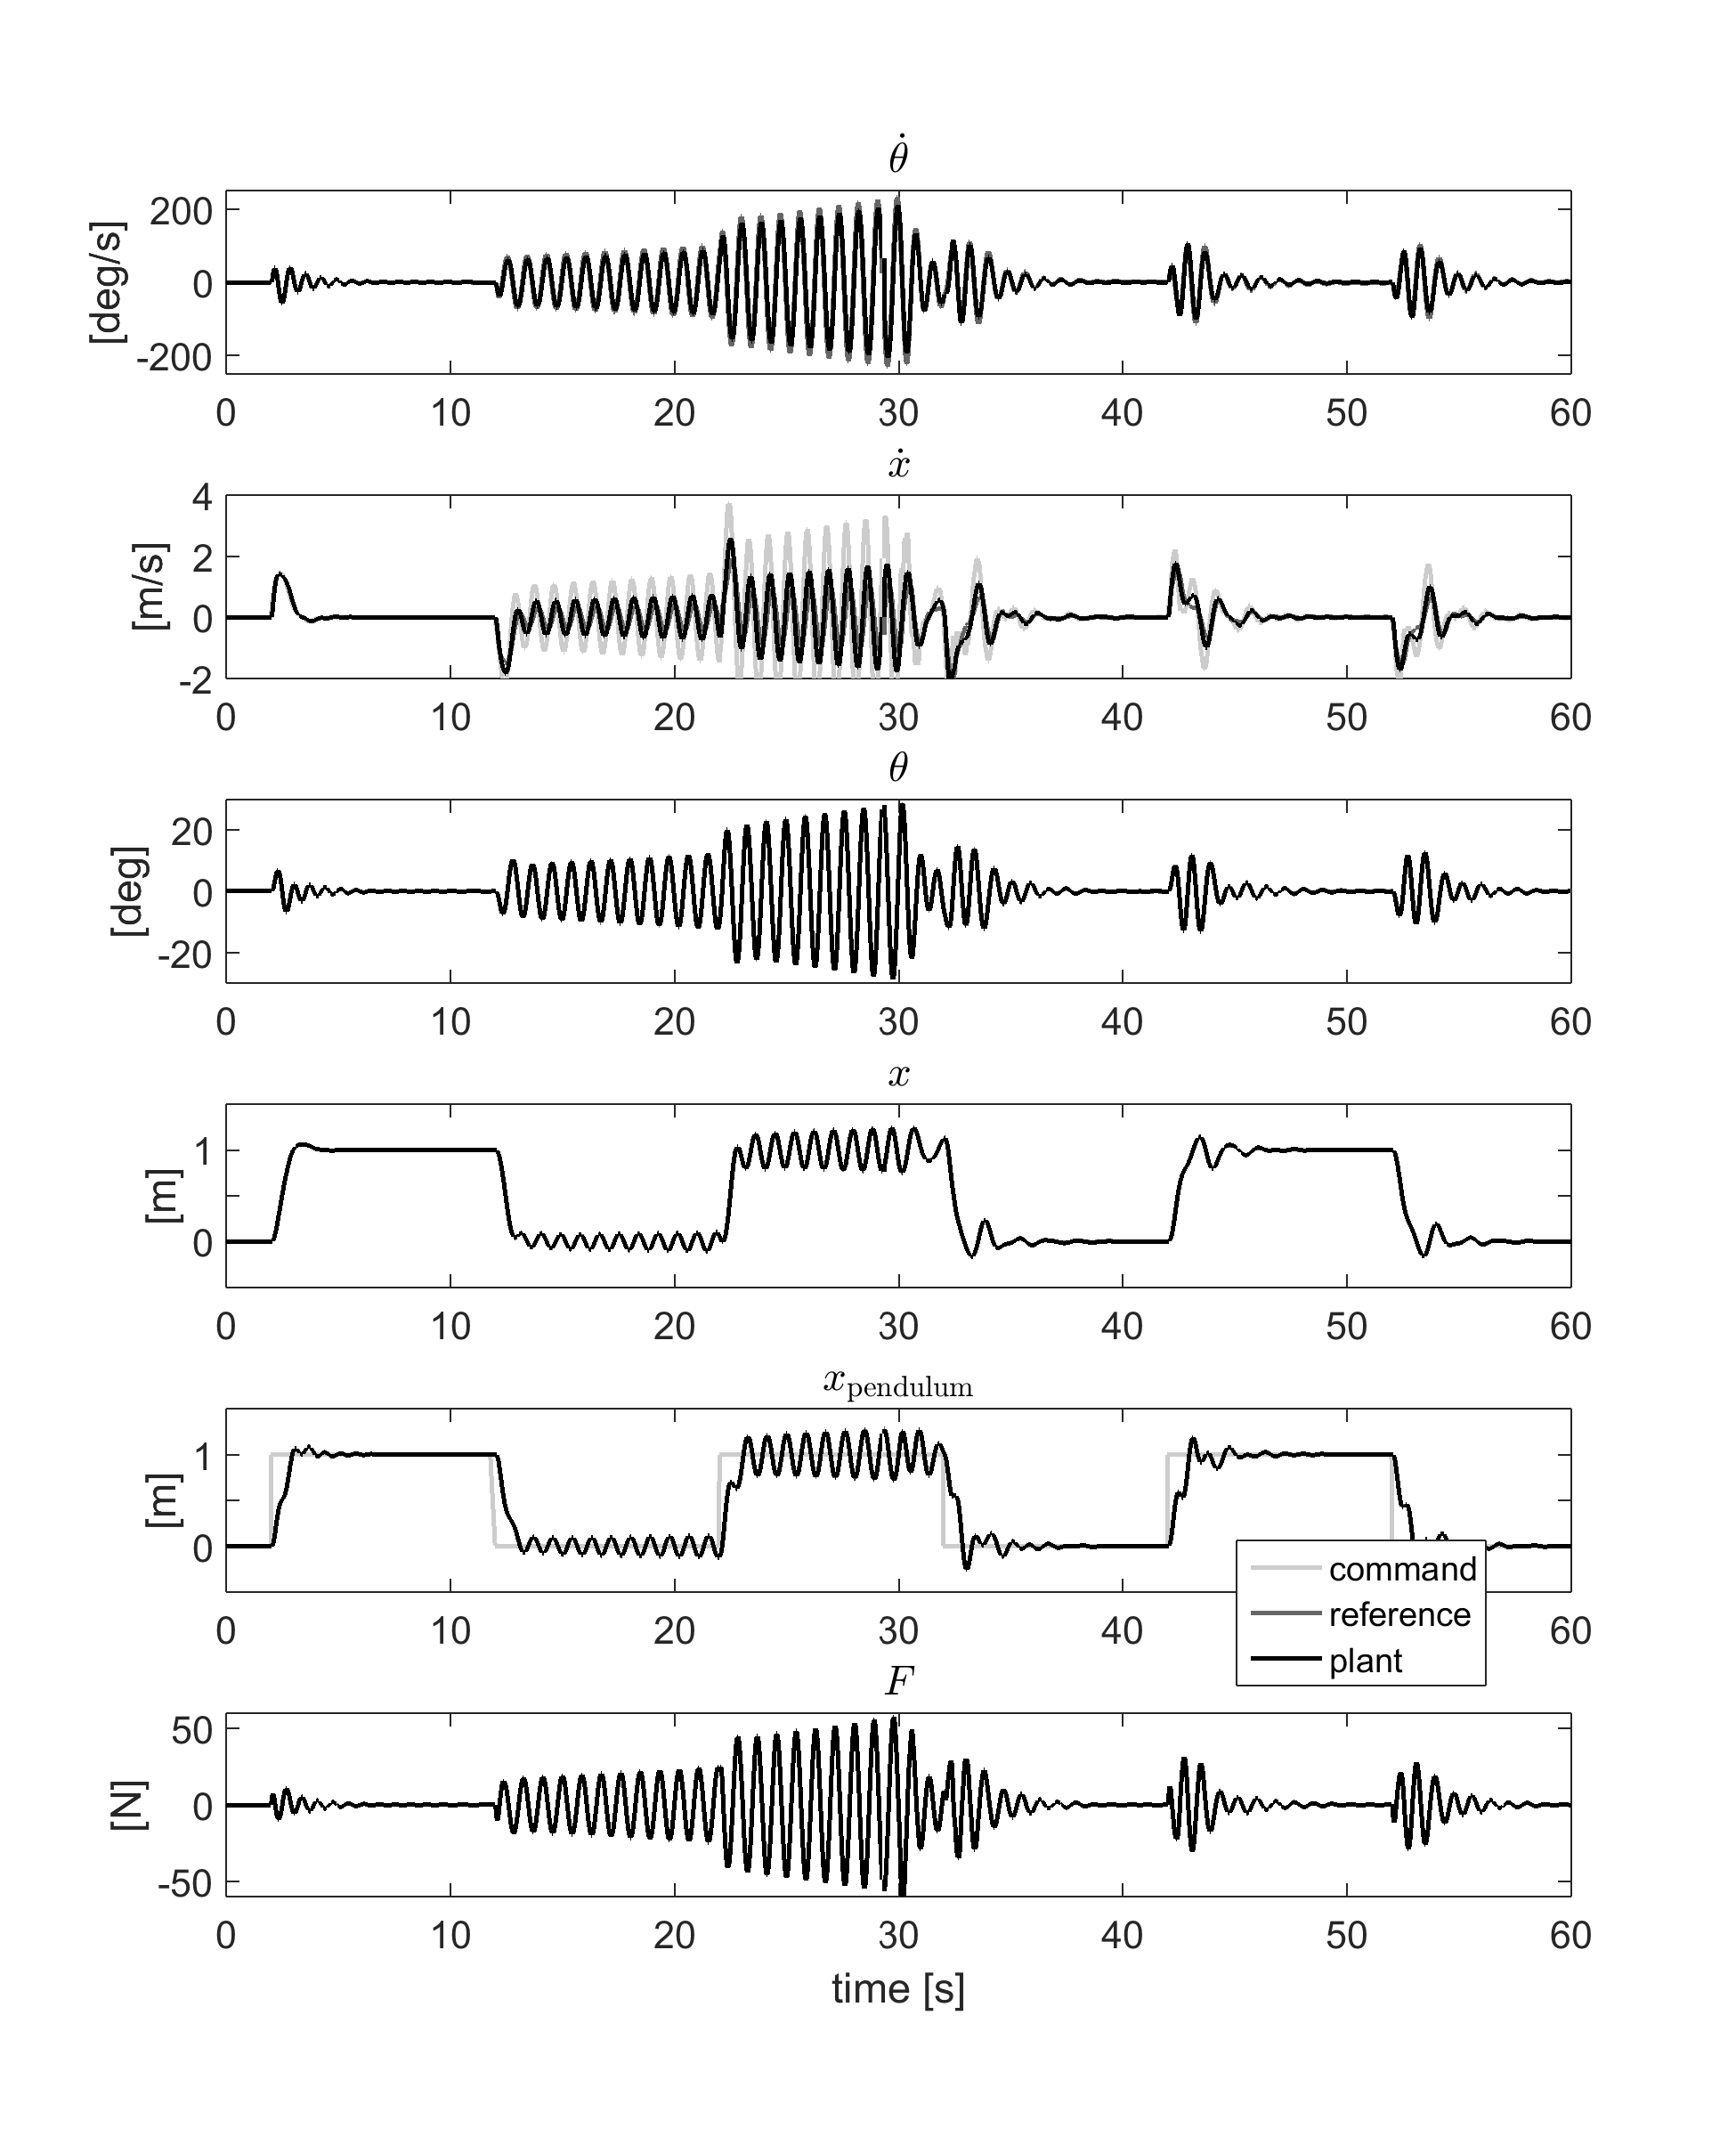
\includegraphics[width=7.0in]{\figurepath/outerLoopPendulumCart.png}}
  \vspace{-0.95in}
  \caption{Time response of pendulum cart with inner and outer-loop controller.\label{fig.outerLoopPendulumCart}}
\end{figure}

\newpage
\begin{figure}[H]
  \hspace{-0.25in}
  \noindent\makebox[7.0in]{%
  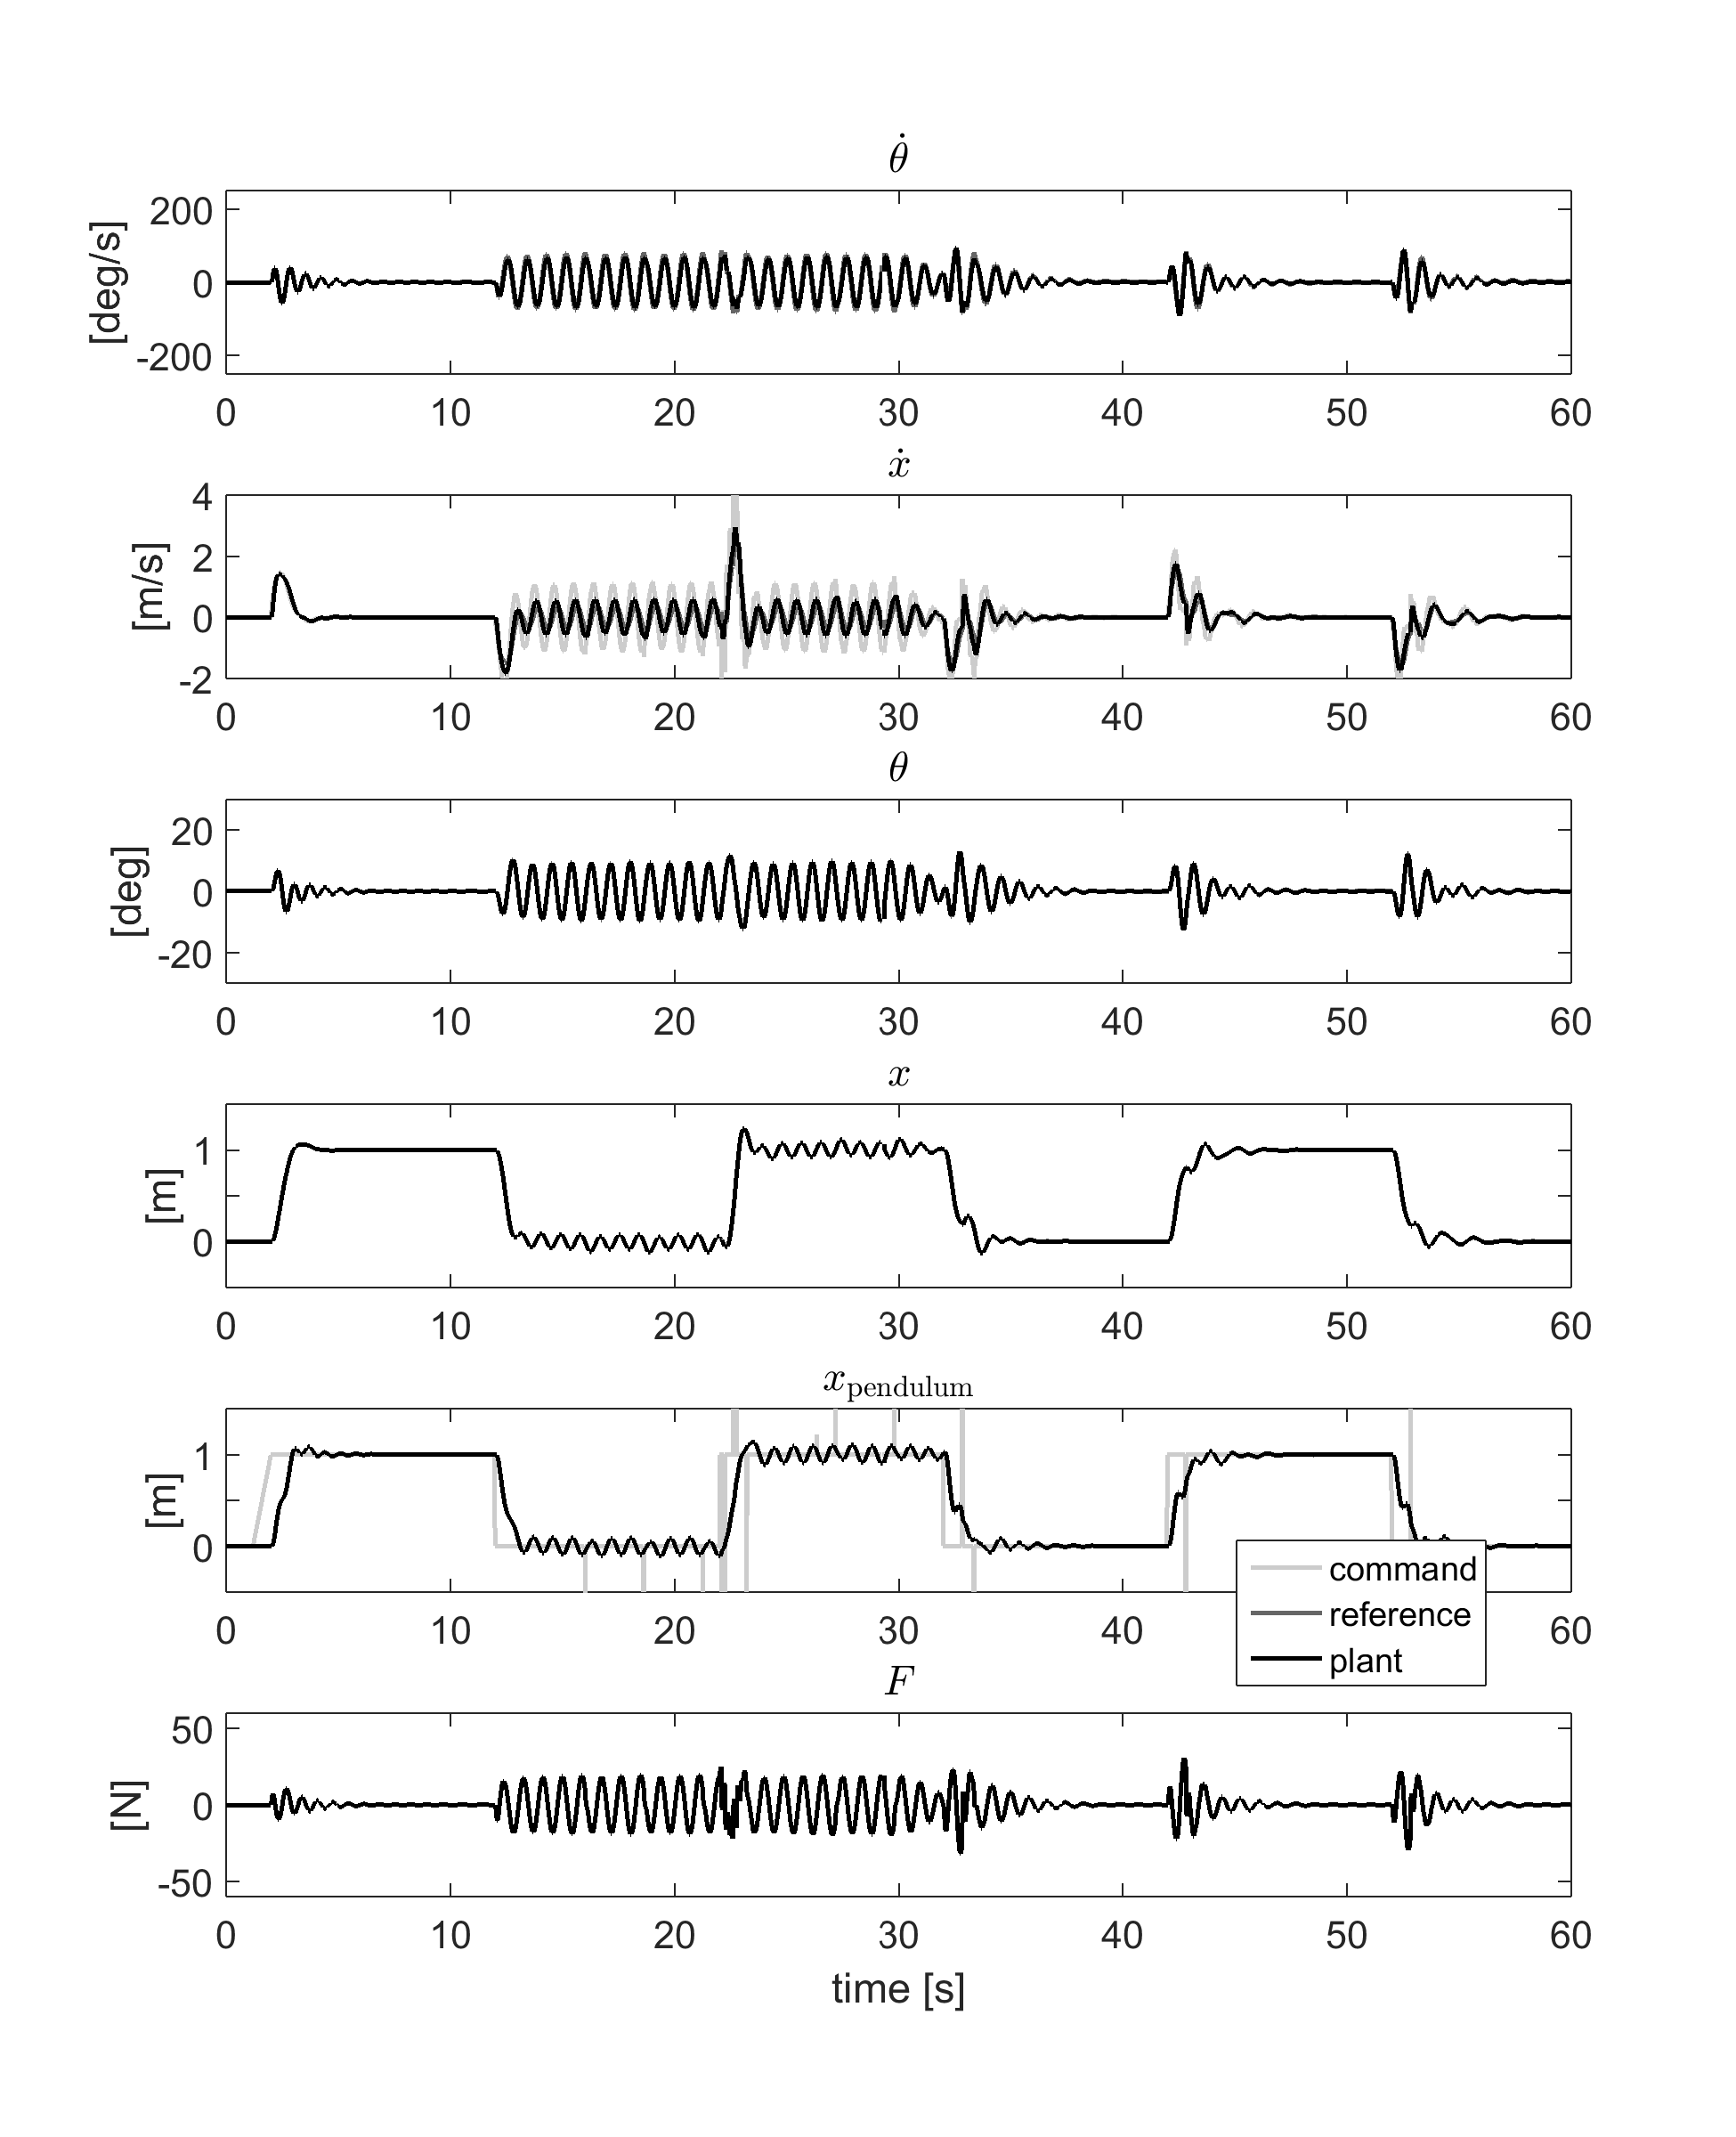
\includegraphics[width=7.0in]{\figurepath/outerLoopStateLimiterPendulumCart.png}}
  \vspace{-0.95in}
  \caption{Time response of pendulum cart with inner and outer-loop controller and state limiter.\label{fig.outerLoopStateLimiterPendulumCart}}
\end{figure}

\subsection{Example 2: Longitudinal Dynamics of a Transport Aircraft}

\begin{figure}[H]
  \begin{center}
    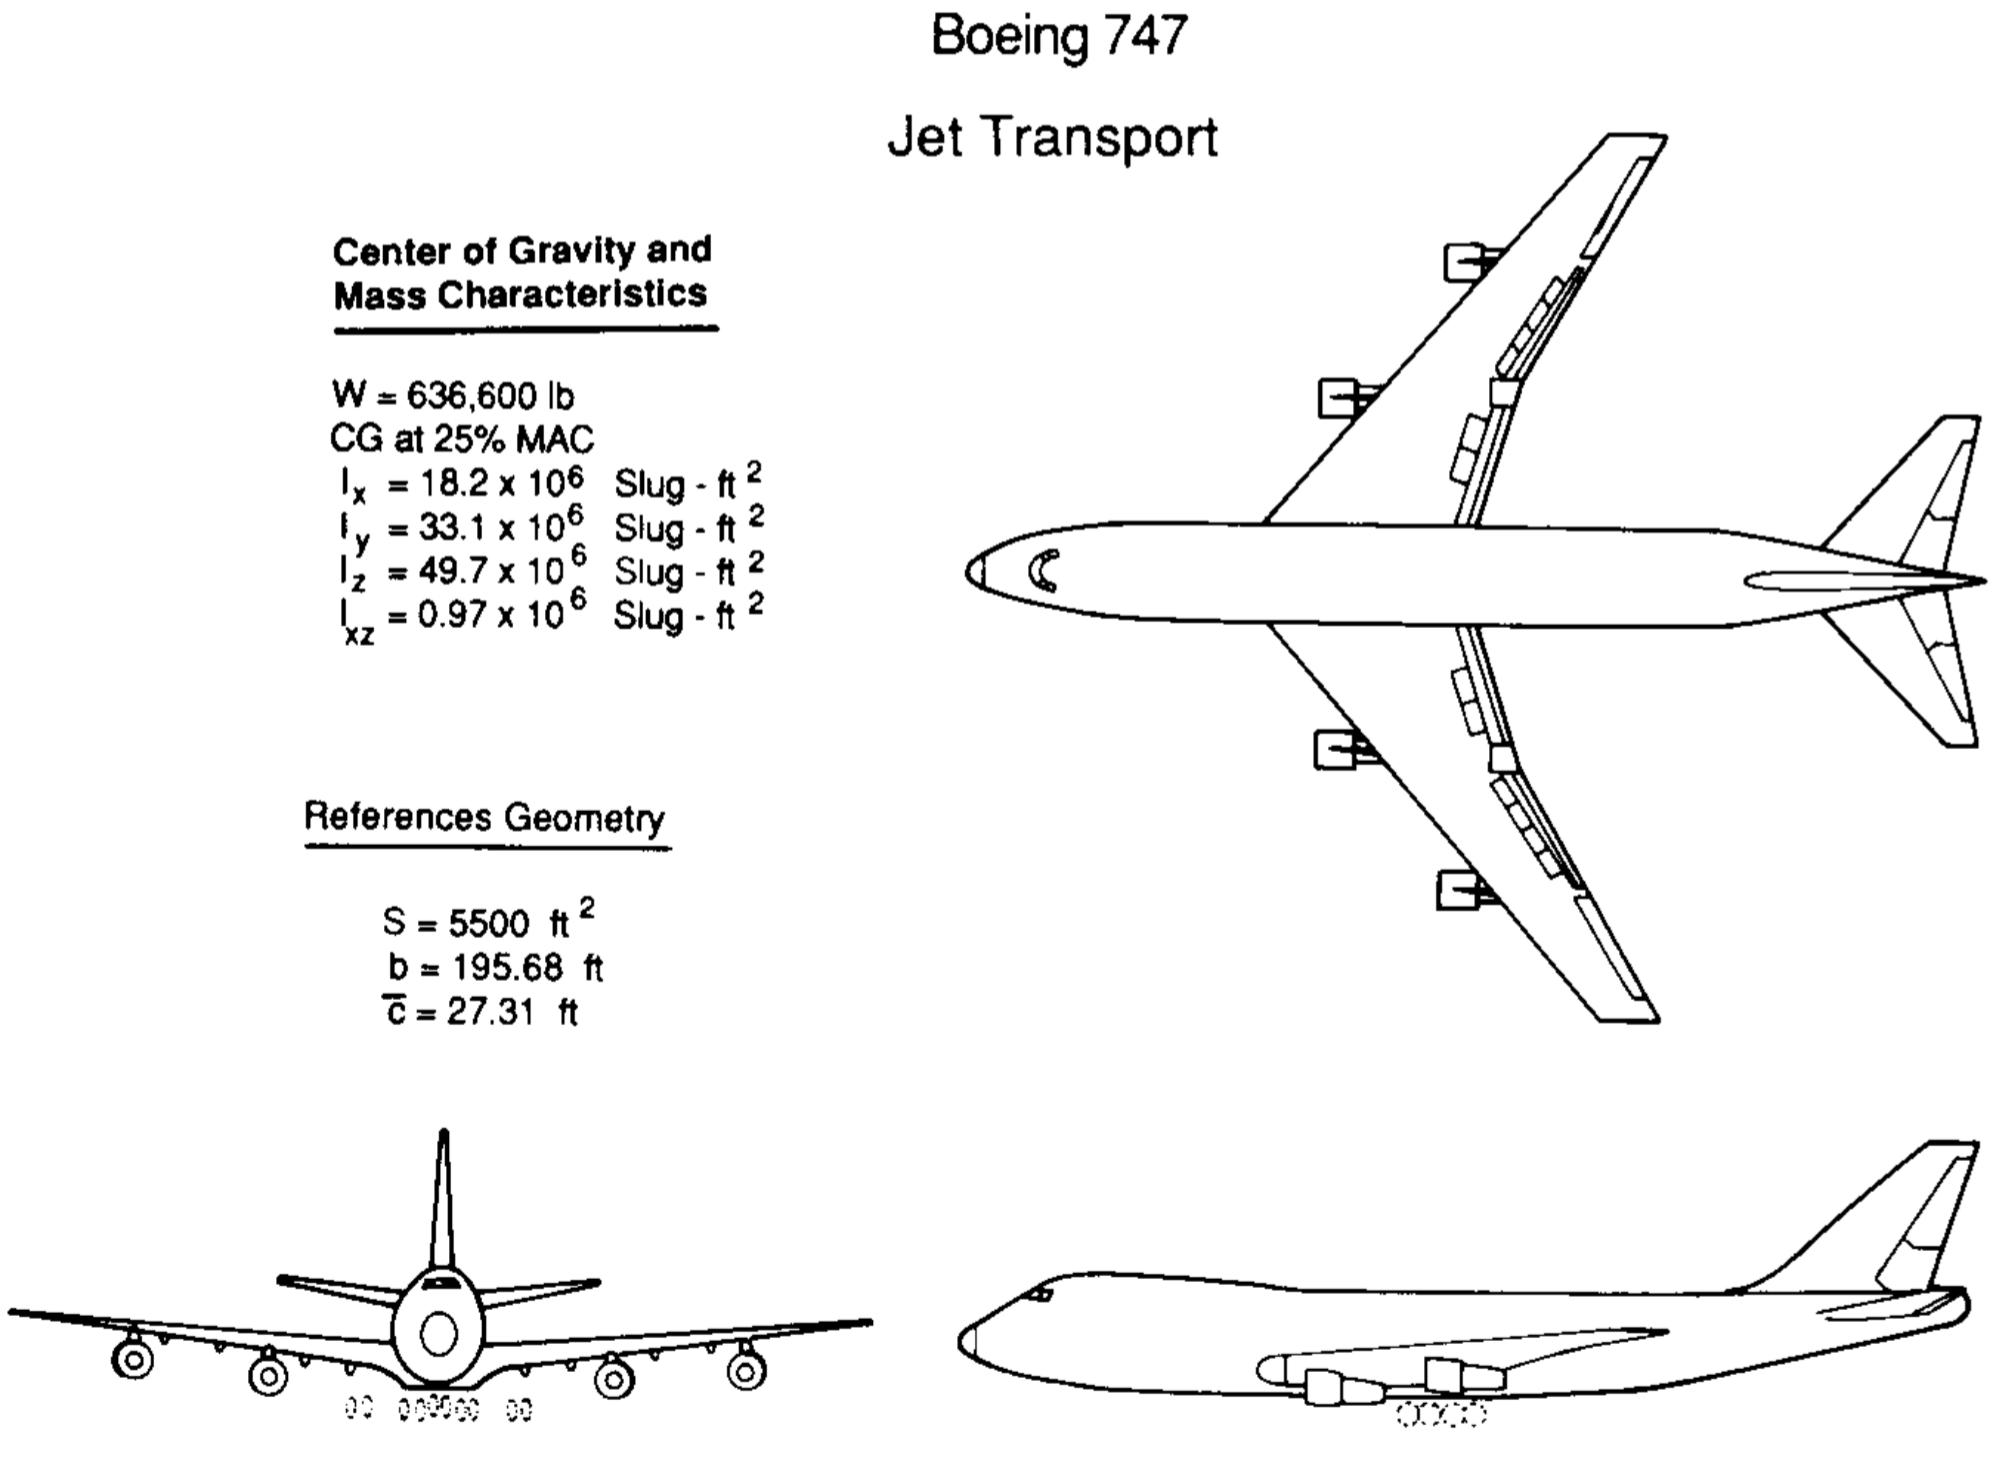
\includegraphics[width=4.5in]{\figurepath/transportLong.png}
    \vspace{-0.1in}
    \caption{Boeing 747--100 transport aircraft from Ref.\ \cite{nelson.flightcontrol.1998}.\label{fig.transportLong}}
  \end{center}
\end{figure}

The longitudinal dynamics of a transport aircraft example from Section~\ref{sec.innerLoopNumericalExample} is continued here.
In the first part of this example, the inner-loop adaptive controller was used to accommodate uncertainties in the moment coefficients and elevator effectiveness, and enforced tracking of the pitch rate commands.
The example is continued here using the plant with this adaptive inner-loop, and the outer-loop controller prescribe the necessary pitch rate command so as to track altitude commands.

The longitudinal aircraft dynamics in\ \eqref{eqn.transportAircraftWhole} were partitioned into the inner-loop dynamics in\ \eqref{eqn.transportAircraftInnerLoop} and the outer-loop dynamics in the form of\ \eqref{eqn.outerLoopDynamics} given in\ \eqref{eqn.transportAircraftOuterLoop} below
\begin{equation}
  \label{eqn.transportAircraftOuterLoop}
  \begin{split}
    \begin{bmatrix}
      \dot{\theta} \\
      \dot{h}
    \end{bmatrix}
    &=
    \begin{bmatrix}
      0 & 0 \\
      v_{\text{eq}} & 0 \\
    \end{bmatrix}
    \begin{bmatrix}
      \theta \\
      h
    \end{bmatrix}
    +
    \begin{bmatrix}
      0 & 1 \\
      -v_{\text{eq}} & 0 \\
    \end{bmatrix}
    \begin{bmatrix}
      \alpha \\
      q
    \end{bmatrix} \\
    h
    &=
    \begin{bmatrix}
      0 & 1
    \end{bmatrix}
    \begin{bmatrix}
    \theta \\
    h
    \end{bmatrix}
  \end{split}
\end{equation}
The matrix $B_{gd}$ which couples the outer-loop kinematics into the inner-loop dynamics in this example is identically zero.
Using the numerical values for the aircraft given in Section~\ref{sec.innerLoopNumericalExample}, the relevant matrices are given by
\begin{equation*}
  A_{g} =
  \begin{bmatrix}
    0 & 0 \\
    871 & 0
  \end{bmatrix}
  \qquad
  B_{gp} =
  \begin{bmatrix}
    0 & 1 \\
    -871 & 0
  \end{bmatrix}
  \qquad
  C_{g} =
  \begin{bmatrix}
    0 \\
    1
  \end{bmatrix}^{\top}
  \qquad
  C_{gz} =
  \begin{bmatrix}
    0 \\
    1
  \end{bmatrix}^{\top}
\end{equation*}
The forward-loop reference model was designed using integral action on the regulated output as in\ \eqref{eqn.rKbar} using the following weighting matrices
\begin{equation*}
  \begin{split}
    Q_{\text{lqr}}
    &=
    \text{diag}\bigr(
    \begin{bmatrix}
      0 & 10 & 0 & 0 & 10 & 10
    \end{bmatrix}
    \bigr) \\
    R_{\text{lqr}}
    &=
    10^{8}
  \end{split}
\end{equation*}
Using the outer-loop design procedure summarized in Section~\ref{sec.outerLoopDesignProcedureSummary}, $P_{g}$ was calculated as in\ \eqref{eqn.Pg} using $P$ calculated as in\ \eqref{eqn.P} and $X_{D}$, where $P_{\Lambda}$ in\ \eqref{eqn.P}, and $X_{D}$ was selected as
\begin{equation*}
  X_{D}
  =
  \begin{bmatrix}
    100 & 0 \\
    0 & 100
  \end{bmatrix}
  \qquad
  P_{\Lambda}
  =
  \begin{bmatrix}
    1 & 0 \\
    0 & 1
  \end{bmatrix}
\end{equation*}
With the resulting $P_{g}$, $S_{g}$ was determined using\ \eqref{eqn.SgCaseI}, and $L_{g}$ obtained numerically satisfying\ \eqref{eqn.condition4a}.
Finally $L_{y}$ was computed using\ \eqref{eqn.Ly} thus completing the outer-loop control design.

The following plot in Fig.~\ref{fig.outerLoopTransportLong} shows the response of the closed-loop system to track altitude commands, when subject to the same uncertainties described in Section\ref{sec.innerLoopNumericalExample}.
The plot shows the baseline controller applied to the nominal plant until $t=90$ seconds when the uncertainty is introduced.
At $t=110$ seconds the adaptive controller is turned on.
As in the inner-loop example, the adaptive element ensures stability in the presence of the uncertainty, and outer-loop command tracking is provided.
However, in Fig.~\ref{fig.outerLoopTransportLong} during the transients a pitch rate of 30 deg/s is experience.
In Fig.~\ref{fig.outerLoopStateLimiterTransportLong} the state limiter is used to enforce the pitch rate to within 15 deg/s.

\newpage
\begin{figure}[H]
  \hspace{-0.0in}
  \noindent\makebox[6.5in]{%
  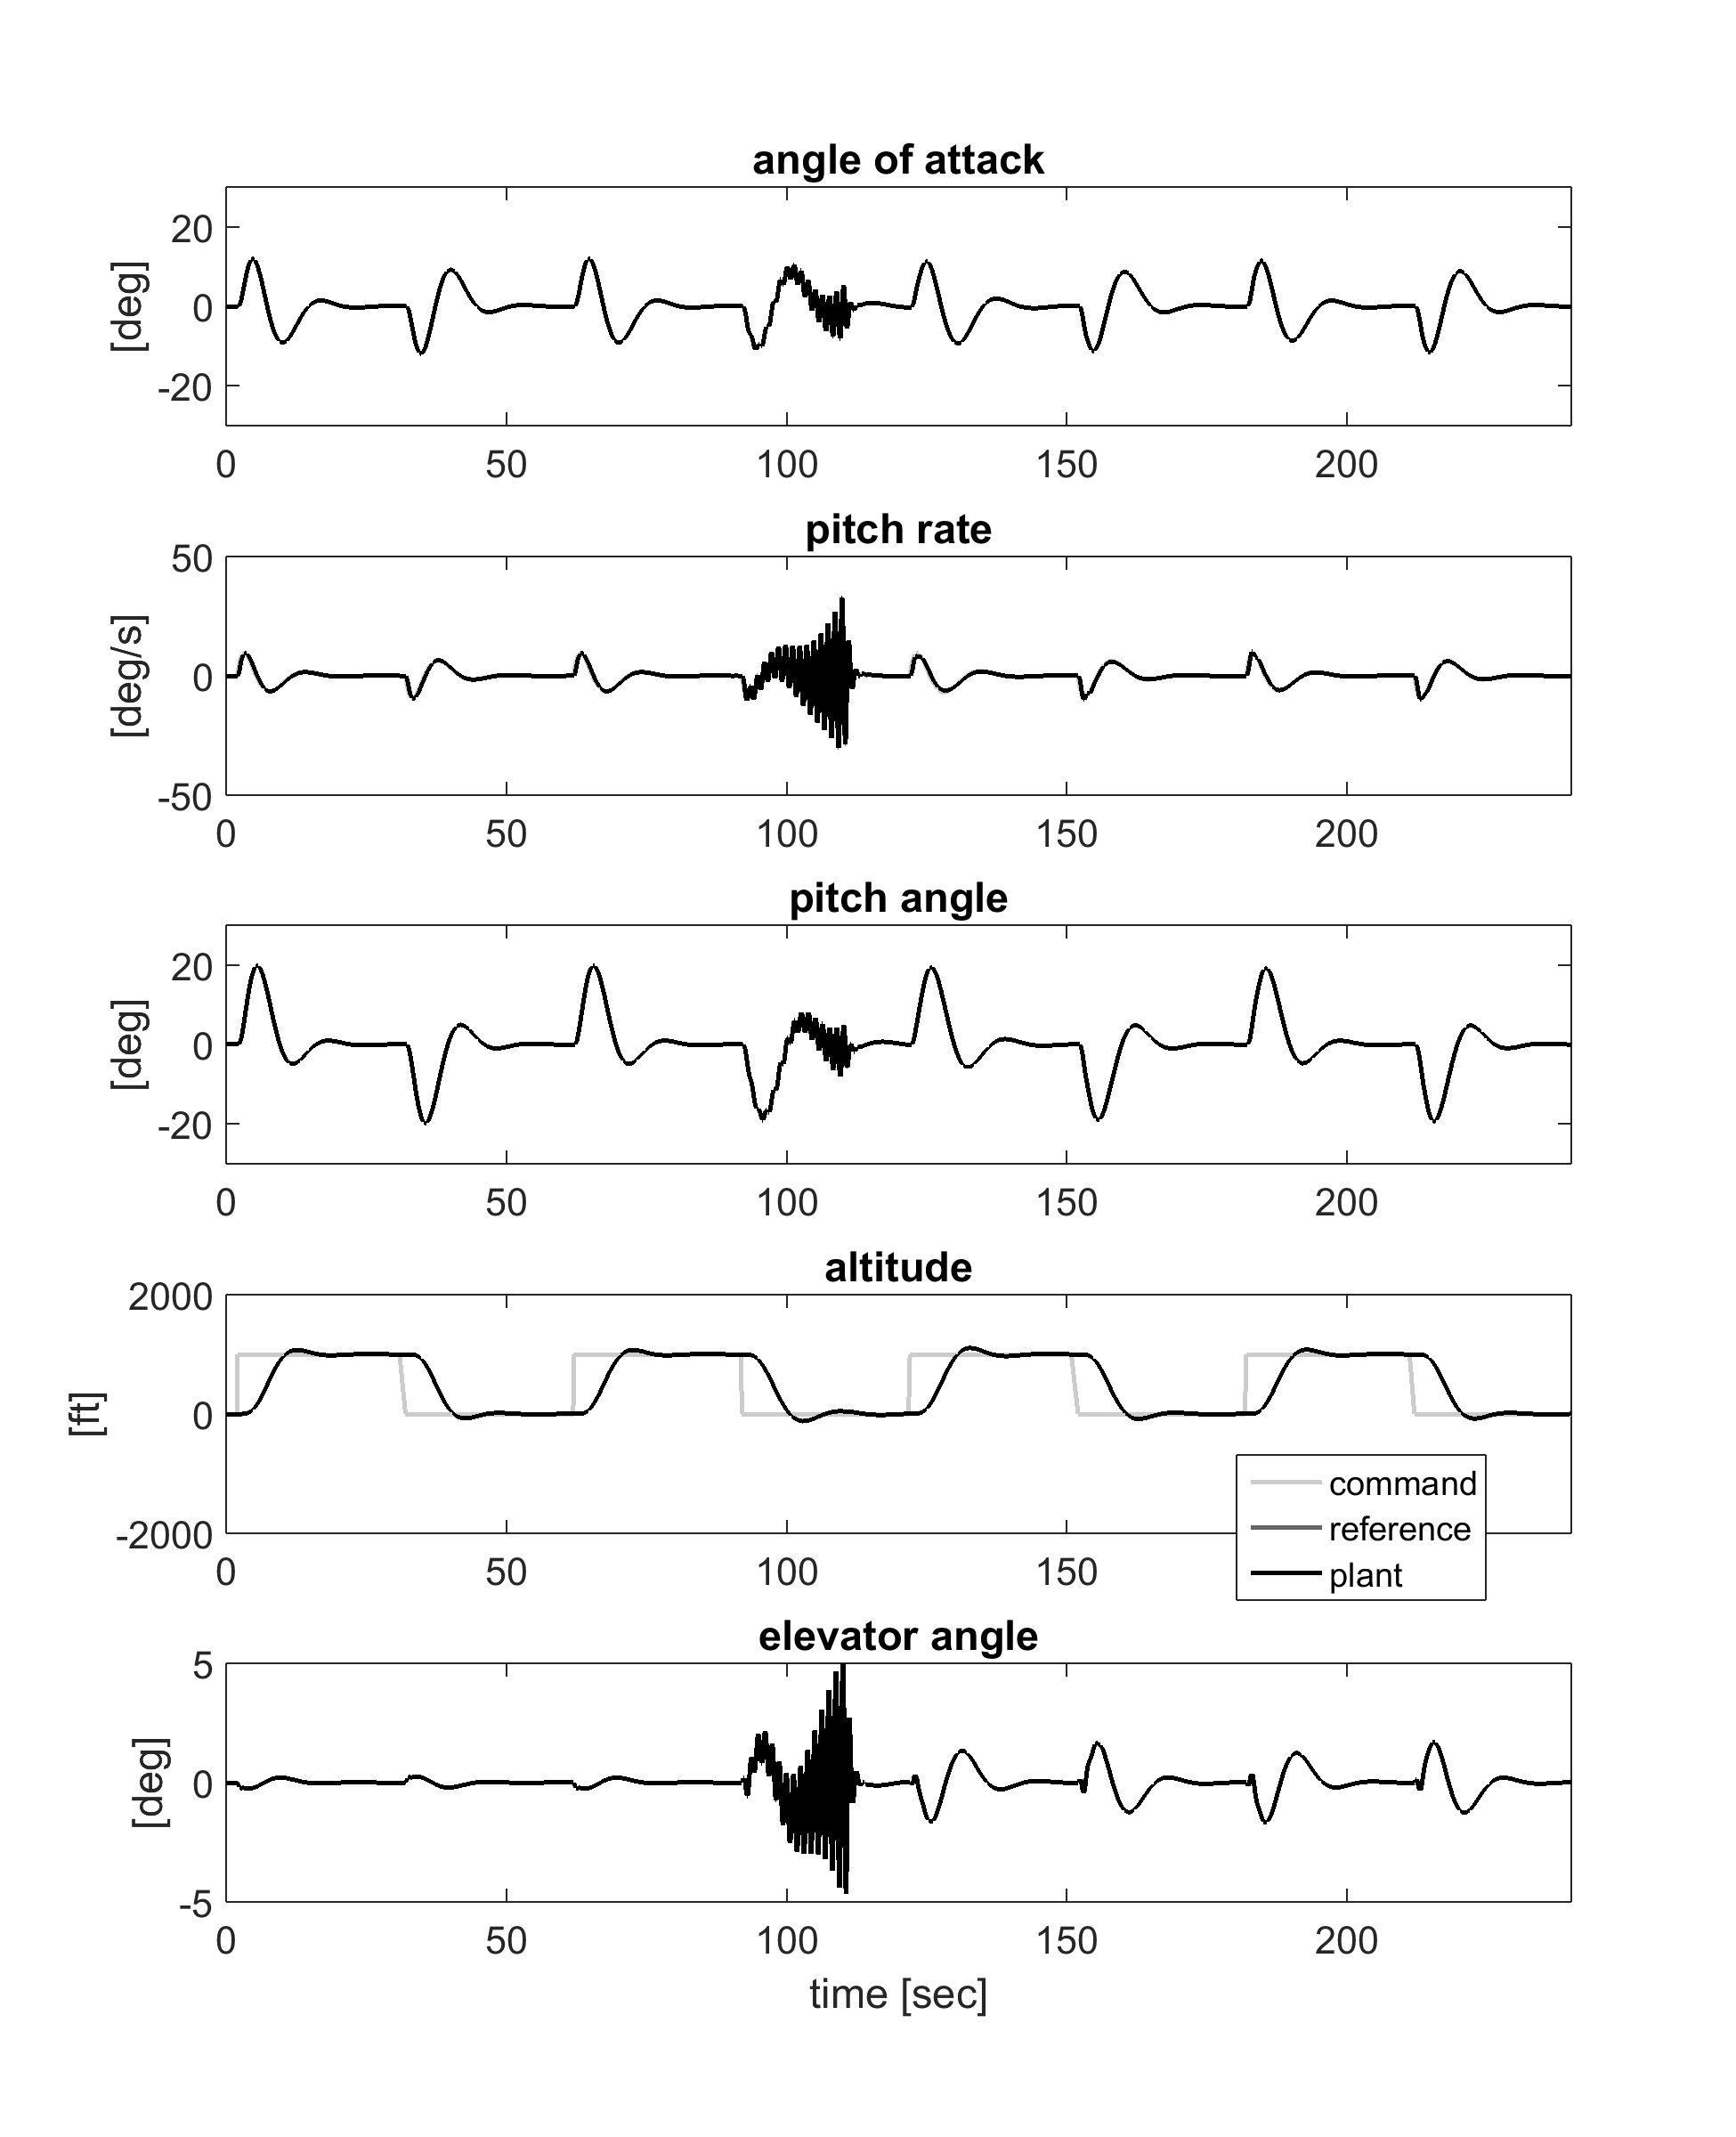
\includegraphics[width=6.5in]{\figurepath/outerLoopTransportLong.png}}
  \vspace{-0.95in}
  \caption{Time response of transport aircraft with inner and outer-loop controller.\label{fig.outerLoopTransportLong}}
\end{figure}

\newpage
\begin{figure}[H]
  \hspace{-0.0in}
  \noindent\makebox[6.5in]{%
  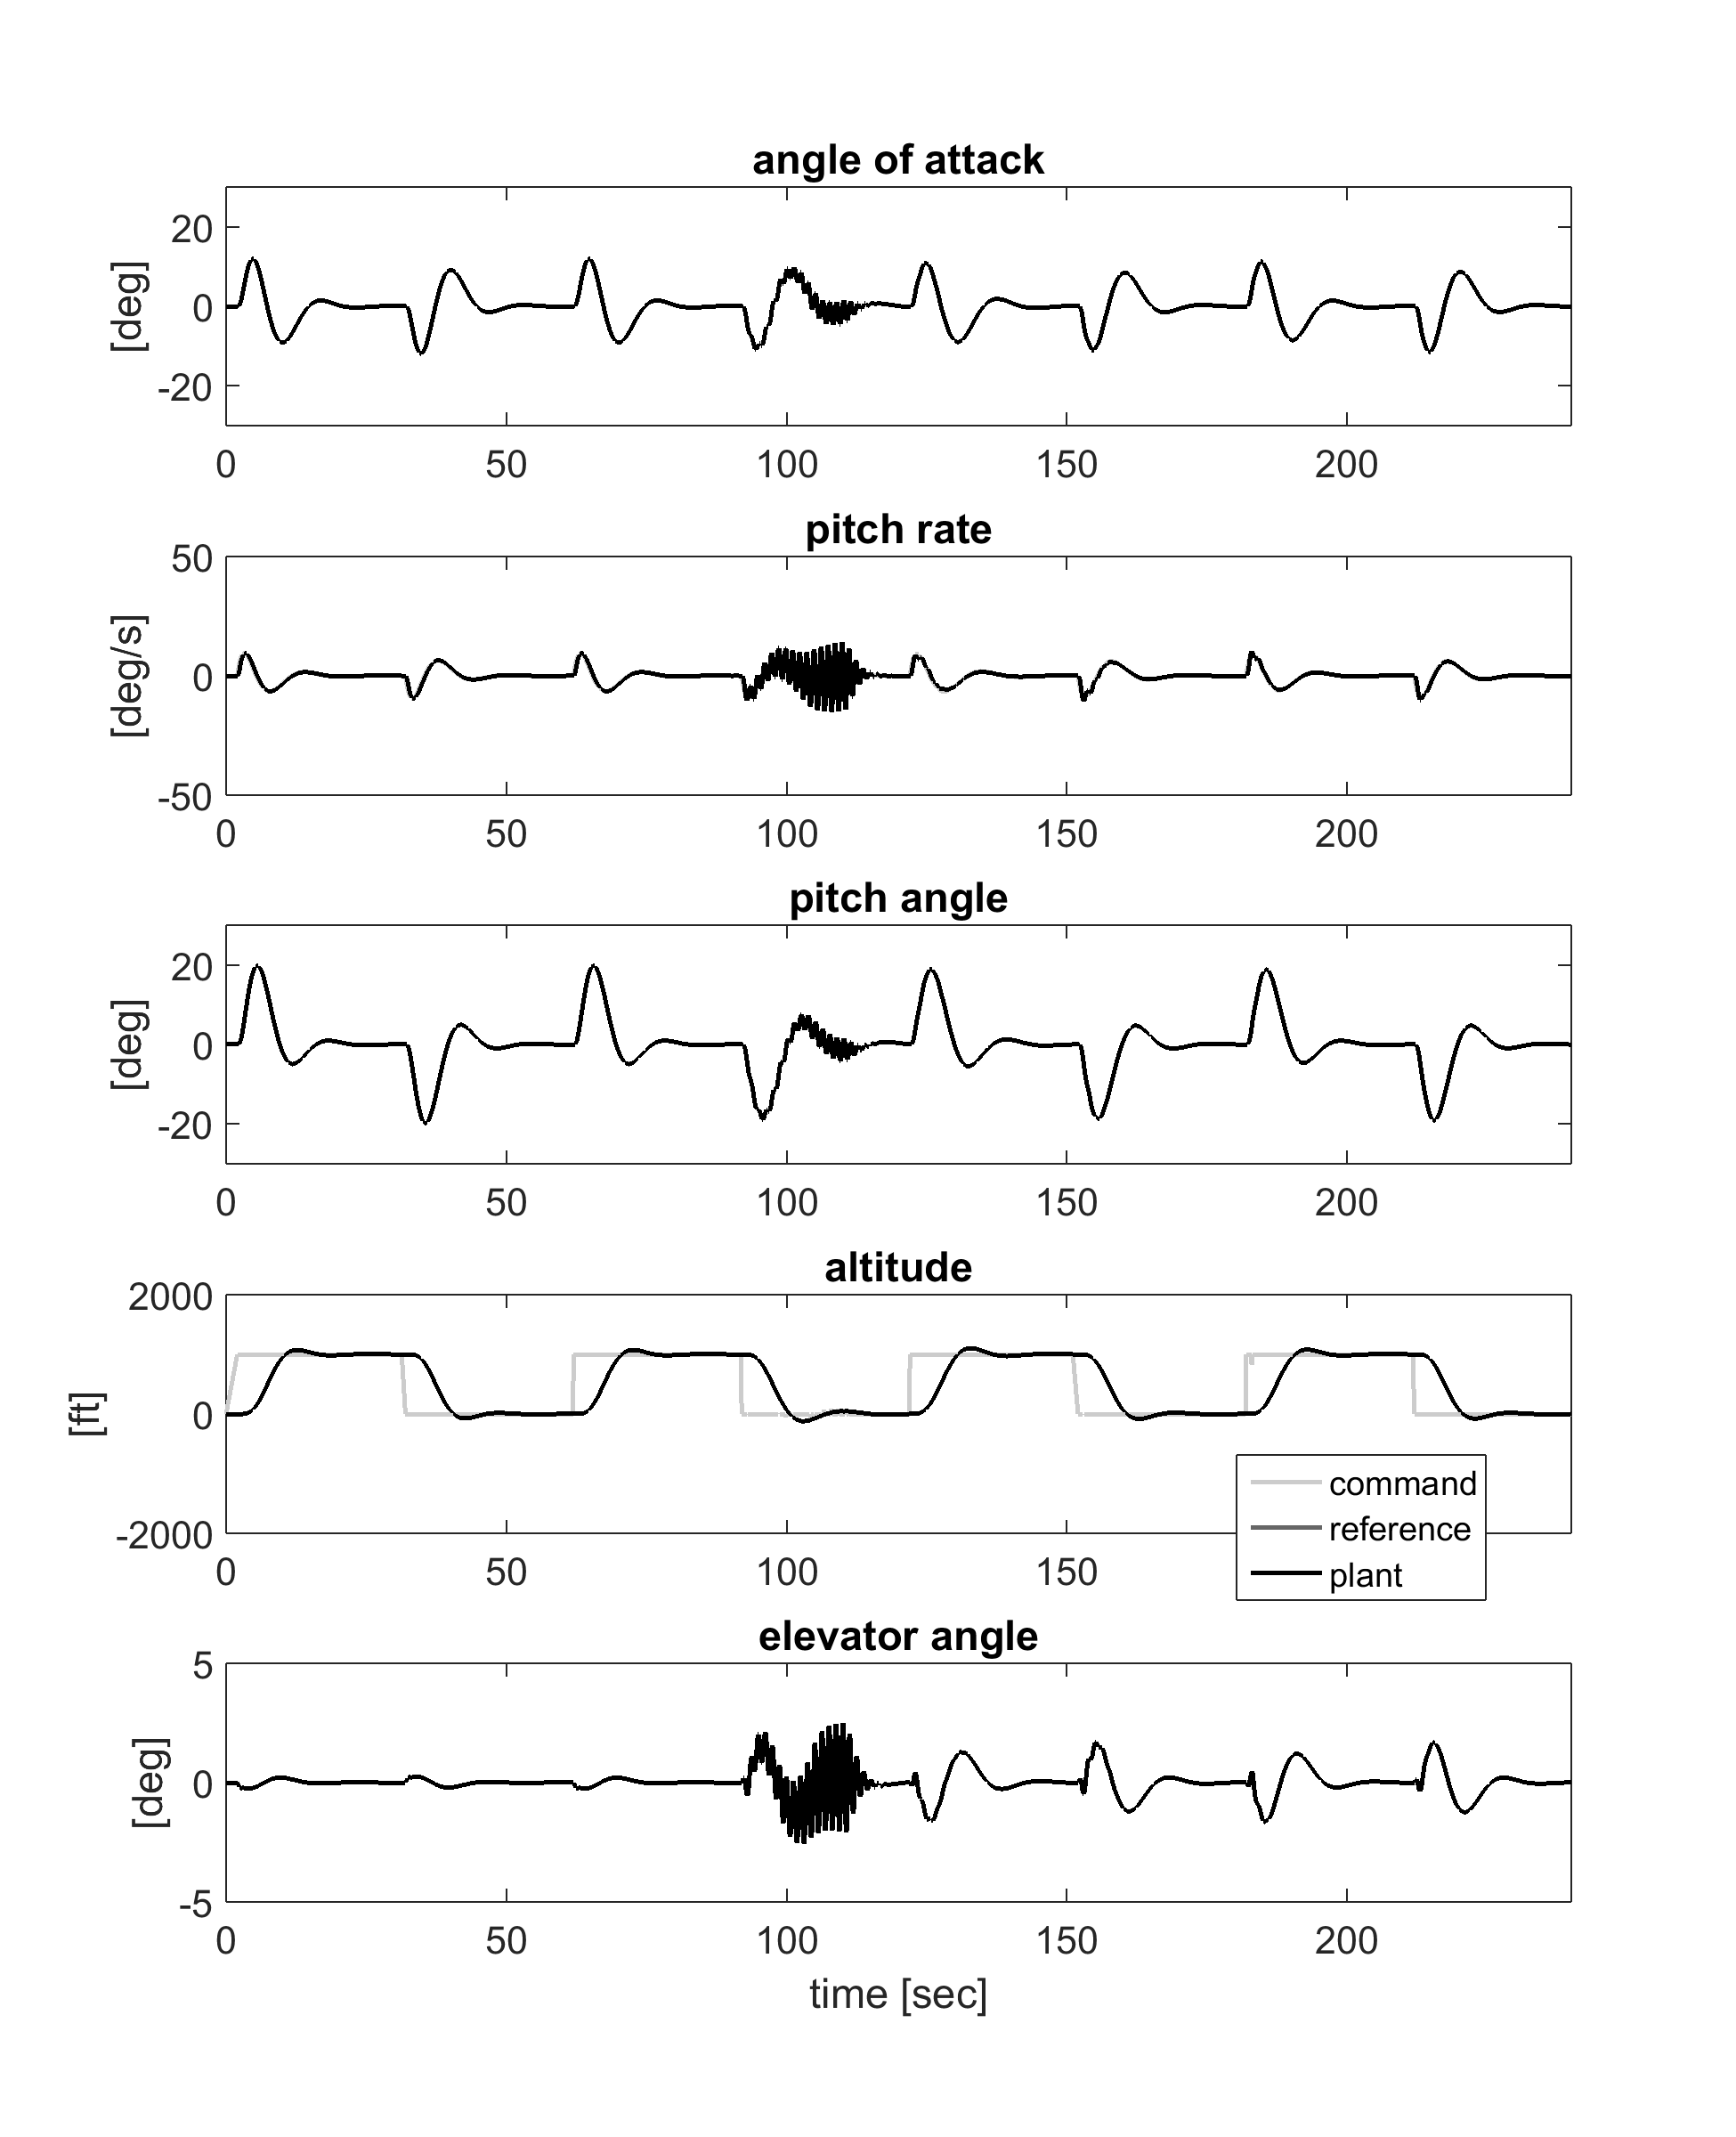
\includegraphics[width=6.5in]{\figurepath/outerLoopStateLimiterTransportLong.png}}
  \vspace{-0.95in}
  \caption{Time response of transport aircraft with inner and outer-loop controller and state limiter.\label{fig.outerLoopStateLimiterTransportLong}}
\end{figure}

\section{Conclusion}

This chapter presented a new method for developing an outer-loop controller for a class of uncertain MIMO systems.
Using the existing inner-loop adaptive control design presented in Ch.~\ref{ch.innerLoop}, this chapter described how to specify the command $z_{p,\text{cmd}}(t)$ to the inner-loop such that $z_{g}(t)$ tracks $z_{g,\text{cmd}}^{\prime}(t)$.
The controller is composed of additional reference model dynamics corresponding to the outer-loop dynamics, and additional CRM gains to suitably modify the outer-loop reference model trajectories to ensure global stability, and provide command tracking of the outer-loop command.
Specifically, these CRM gains were chosen so as to stabilize the outer-loop reference model, and then decouple the inner and outer-loop error dynamics.
Synthesis of the CRM gains involved satisfying a matrix equality and an bilinear inequality, to provide the desired error decoupling, and outer-loop reference model stability.
Using the matrix elimination lemma as in Ch.~\ref{ch.innerLoop}, the BMI was reduced to an LMI, and the problem of determining the CRM gains was reduced to finding a positive definite matrix $P_{g}$ which satisfied the LMI, with the additional constraint that $P_{g}$ also satisfy the matrix equation $\Pi_{A}P_{g}\Pi_{B}=\Pi_{C}$.
The set of all solutions which satisfied these constraints was given in terms of an arbitrary matrix $X_{D}$.
The set of all $X_{D}$ which ensured a stable outer-loop controller was large, allowing the extra degrees of freedom of $X_{D}$ to be selected to provide the desired level of performance and robustness to the closed-loop system, in addition to stability.
The result is a hierarchical MIMO adaptive output-feedback controller which can be designed to have good stability margins, contains an adaptive element to accommodate uncertainty, and provides the desired command tracking.
Furthermore, the architecture of the hierarchical approach allowed the addition of a state-limiter to the controller, to limit the plant state to certain regions in the state space.

In Ch.~\ref{ch.applicationHypersonic} this hierarchical, MIMO adaptive output feedback controller consisting of the inner-loop controller from Ch.~\ref{ch.innerLoop} and the outer-loop controller from Ch.~\ref{ch.outerLoop} is applied to a hypersonic vehicle model.
